% !Mode:: "TeX:UTF-8" 

\BiChapter{研究可编程设备加速主机侧网络方法}{NIC}


\BiSection{本章引论}{}

\BiSection{问题背景}{aa}

%有什么东西软件做不好的,
%
%为什么要选流量工程 和 压缩加速。一定要好好想明白。 每包计算是最费劲儿的。
%流量系统背景和测量背景, %1
%
%软件流量捕捉 回放能力,

随着数据中心服务器网络接口容量快速增长,处理与网络数据相关的服务已越来越耗费主机CPU的计算资源。主机虚拟化、流量工程、网络监管等功能在现代化网络管理中已经占据重要的位置。尽管目前发展出一系列RDMA、DPDK等基于网卡的网络数据包快速搬运架构,但它们只针对于块儿数据的传递进行了优化,对于需要“每包处理”的任务依然没有良好的对策。



本文将复杂网络计算问题分为两类任务类型,一种类型是由于数据包到达频繁而触发的大量计算,也许这类型计算并不复杂(处理器使用几条指令即可完成计算),但由于需要对每个数据包都进行处理从而导致计算量庞大、CPU无法胜任,例如查找、转发、分类等。第二种类型是由于计算过程复杂(处理器需要耗费多条指令才可完成计算),导致CPU无法提升针对每个数据包处理的速度,进而造成网络分发数据包个数降低、性能需求无法胜任,例如防火墙、安全分析等。数据中心运营商面对着不断增长的功能需求和性能需求,同时也面对着需要降低运营成本提升能源利用率和绿色环保。

网络随路计算(in-network computing)是一种解决网络程序性能差的有效途径。网络随路计算是指在网络数据传输链路中增加特定功能的硬件设备,使得数据包在传送到主机内部之前,就完成了网络任务中的相关计算需求。当计算从主机内,下方到了网络内后,这便释放了软件处理瓶颈,可以节约数据中心内宝贵的CPU处理资源。但主机内的计算任务并不能够全都被硬件卸载,因而我们需要选取可编程数据平面来完成这件事。前文提到过三类可编程网卡他们分别是:基于可编程ASIC的智能网卡,基于NPU的智能网卡,以及基于FPGA的智能网卡。首先本文分析基于ASIC的智能网卡是非“图灵完全”的可编程硬件,尽管其处理性能优异,但无法支持灵活配置,因而本文不考虑。其次基于NPU的智能网卡,NPU由众核处理器架构组成,可提升处理并行度,但这是基于批处理的计算模型。针对目前流式计算和有状态计算,因NPU每核处理性能低,从而导致NPU方案整体运行性能差。

本文从上述两类问题中各选取了一个应用场景,来说明使用基于FPGA的智能网卡具更高精度的“每包处理”能力,以及强大的“复杂计算”能力。最重要的是FPGA可以支持网络内流式计算模型,本文在后面提出了一种在FPGA针对流式计算需求的DC抽象方法,可以将有前后状态依赖的“复杂计算”任务卸载到基于FPGA的可编程硬件。

%The Case For In-Network Computing On Demand 分类举例说明



\BiSection{系统架构}{aa} %1

\BiSubsection{软件向硬件卸载分析}{aa}

CPU通过循环取指令等操作,完成通用的可计算任务。计算的数据通常有前后依赖关系,CPU对于此类计算效率较低:由于中间计算状态在计算完成之后必须放回数据存储区,而下次重新拿回状态数据又需要再次搬运,数据在计算核心与存储池之间多次往返对计算最终结果是无意义操作。而即使使用众核处理器也无法优化此过程,虽然众核处理器可并行计算多个任务,但同一时刻每核心与其他核心处理内容并无关联。对于前后有依赖关系的处理,并行并不能加速其中一组数据的处理进程。在网络领域亦是如此,网络数据包到达密度很大,留给每个包的处理时间很有限,然而通常一个CPU无法在如此短时间内真正处理完一个包的触发计算。


1)软件处理延迟大。

目前高速网络处理器可以设计为核间流水线模式,每个核只处理固定的一步计算。当一个数据包触发的计算包括多个前后依赖计算时,人们使用多个核串行处理这组计算。即每个核心领取一个固定的快速处理任务,这样每个核都可以以最快的速度处理完当前步骤,然后交给后续核心继续处理。这样数据包的处理吞吐其实就可以达到某一个核心的最大速度,而处理延迟则是这些核心之间传递完整一次的时间。不难发现,数据在众核之间搬运会遇到访存时间过长、访存请求冲突等现象。虽然使用CPU可以获取很大的灵活性,但这种方式进一步增大了每个数据包处理的时延。如今在云端加速AI计算的场景下,高频次小包、数据快速到达的需求越来越高,这使得以CPU处理网络数据包造成很大的云计算性能瓶颈。后续我们通过本文所举的例子可以明显提现这一点。

2)软件处理时间精度低。

同时,由于共享内存与总线架构,数据在CPU核心、存储池之间搬运会造成随机的请求冲突、甚至计算等待,这将中断顺序串行处理节拍。由于这条处理链中的处理速度会受到这条处理链最慢处的制约,因而处理链的性能表现总以最慢的瓶颈向外表现。
软件的处理收到操作系统的指挥,操作系统一般会划分时间片区来分配给每一个待处理的任务。虚拟化的操作系统内有很多任务进程,操作系统会划分很多时间片区。这也进一步降低了CPU的专用任务处理性能,还带来处理时间精度不足的现象。后续我们通过本文所举的例子可以明显提现这一点。

3)软件功能向硬件卸载。

卸载是指将工作负载从一个实体转移到另外一个实体上去。软件功能的卸载遵循一定原则:

\begin{itemize}
	\item 新实体可以做与原来实体相同的工作,但资源耗费更少。
	\item 新实体比另外一个实体更快地完成某种类型的工作。
	\item 新实体有能力做除此外的其他任务。
\end{itemize}

硬件功能卸载已经广泛使用在计算机领域。早期,开发人已经把音视频处理从CPU完全卸载到图形处理器和音频芯片中。此外还有一些例子:数据包校验计算卸载到网卡,传输大宗数据时使用DMA控制器,在硬盘控制器中做数据错误恢复。事实上,从CPU中卸载出来的功能都比单纯由CPU执行能源效率高很多。但本文并不是强调CPU无用论,因为CPU是整个服务器中最具有灵活性的器件。卸载任务应该是简单、机械的,CPU是系统内可编程、可运行花样繁多的算法,从而具有很高的难以替代性。

卸载通常是一种优化技术,与其他优化方法一样,仅在合适场景下适用,虽然他增强了计算效率,但这种卸载方式并不是完美的:

\begin{itemize}
	\item 增加了软硬开发人员的工程任务量。
	\item 增加新的硬件,使系统结构复杂。
	\item 设计制造新硬件,增加研发周期、增加使用成本。
	\item 由于大量装配特殊器件,系统可移植性降低。
\end{itemize}

对于灵活多变的网络流量的处理任务,大多为分步骤且数据包信息前后依赖关系高。前文提到,如果使用基于NPU的可编程网卡,虽然灵活性可以被满足,但依然存在性能问题(单核性能低,单个数据包处理延迟大)。使用基于可编程硬件(FPGA)的智能网卡卸载网络功能,可以有效解决上述问题。


\begin{table}[!ht]
	\renewcommand{\arraystretch}{1.2}
	\centering\wuhao
	\caption{FPGA的优势与劣势} \label{table:FPGAstrengthandweakness} \vspace{2mm}
	\begin{tabularx}{\textwidth}{*{2}Y}
		\toprule[1.5pt]
		FPGA所擅长的处理内容 & 不适宜使用FPGA处理的任务 \\
		\midrule[1pt]
		流式数据通路(视频处理) & 多决策算法 \\
		并行算法 & 递归 \\
		低延迟、确定延迟系统 & 依赖于其他大型软件库 \\
		与硬件接口紧邻 & 急速变化的浮点数学计算过程 \\
		\bottomrule[1.5pt]
	\end{tabularx}
\end{table}

表\ref{table:FPGAstrengthandweakness}展示了使用FPGA作为卸载功能目的实体与CPU和ASIC对比的相对优劣点。虽然FPGA完全有能力完成分支多且复杂的决策算法,但相比于CPU,在FPGA上实现会付出更多编码时间,不如使用通用处理器经济收益好。另外相对软件而言,FPGA的处理过程具有精确无抖动(jitter-free)的时序效果。虽然独特优化的软件代码可以近似达到这种效果,但它依然严重地受到调度器,中断,不同处理路径的影响而产生抖动。


\BiSubsection{软件算法的硬件抽象方法}{aa}

在高性能的大数据领域,批处理技术已经可以满足非常多的使用场景,但随着数据时效性价值提升,一种流式计算概念被提出。流式计算是实时的,常驻的,与Hadoop,MaxCompute,Spark等系统不同(它们是离线批处理),流式计算对延迟属性要求更为苛刻。而目前在大数据和高性能网络中的处理就更需要考虑如何利用FPGA来加速流式计算的需求。
%阿里巴巴 大数据page70 流式计算的特点
\begin{figure}[!ht]
	\centering
	
\includegraphics[scale=1]{fpgaprogramabstraction.pdf}
	\caption{FPGA硬件编程抽象} \label{fig:fpgaprogramabstraction}
\end{figure}

1)FPGA编程抽象。
		
基于FPGA的可编程逻辑,可以完成很多种计算。在软件思维转向硬件化的时候,如图\ref{fig:fpgaprogramabstraction}所示,给出了三种并行化加速方法:同一种功能($F(x)$)的复制展开并行;一组数学计算的内部隐含(四则运算分配律和结合律)逻辑并行;分支选择的选路并行。



2)功能卸载的“数据---计算”DC抽象方法。

\begin{figure}[!ht]
	\centering
	
\includegraphics[scale=1]{dcprinciple.pdf}
	\caption{FPGA加速流式计算的DC抽象方法与原则} \label{fig:dcprinciple}
\end{figure}

网络计算卸载到FPGA中,需要在FPGA的并行计算加速基础上,引入一种适合于流式计算FPGA的编程抽象,本文称其为“数据---计算”模型(Data--Computing,DC抽象)。如图\ref{fig:dcprinciple}所示,每个节点内都包括一个或一系列功能(函数$F(x), G(x)$等),本文称其为“计算”,在不同的计算节点之间是数据流(以数据包为驱动),本文称其为“数据”。如何排列和组织这种“计算和数据”是DC抽象的核心内容。一般数字电路会设计为时序逻辑,也就是以时钟周期时间跨度为节拍的计算。各个逻辑块需要在同一个节拍内计算出相应结果。对于在数据处理时前后无关的计算可以归到内部并行中去,所以流式数据处理方法需要挑出数据计算时有前后相关的部分,并把它们按照一定拓扑串联起来。DC抽象基于上述分析提出在FPGA内处理网络流式计算的加速的原则:

\begin{itemize}
	\item 在流水线的每一级具有确定的节拍数。
	\item 数据前后内容具有依赖性。%流式处理要分层,只把前后数据相关的分层,
	\item 有固定的流水线拓扑,但是数据在拓扑间可任意流动。
\end{itemize}

下面将重点介绍本文如何利用DC抽象原则,对基于可编程硬件的网络高时效性网络任务和高密度计算任务卸载加速的研究。

%上面的部分再画个图吧。。。。。。

\BiSection{网络流量捕获与回放}{aa} %4

\BiSubsection{概述}{aa}

网络测量和分析是监控、调试和管理网络,进而设计反馈和优化网络结构以及改善网络服务质量的重要手段。近年来,互联网与网络应用的不断发展,网络内服务器遭遇的各类破坏与攻击也随之与日俱增,网络安全问题日益手段人们的重视。因此,在大型数据中心内,对入侵攻击的检测与防范、保障信息系统和网络系统安全已经成为研究人员的共识。为了快速确定网络攻击的发生,如何设计一种可以实时检测网络流量的网关系统变得异常重要。例如,当网关系统发现大规模DDoS攻击时,可以主动做出丢包等拦截动作,但是对正常数据包应采取放行策略。

这类系统对低传输时延、高吞吐迫切需求。对于复杂网络协议、和内容的分析,一般需要使用大型服务器的多核CPU。由于网络中流的数目很多,因此可以将不同的流量分配到不同的并行CPU中去做并行入侵检测。但对极高流速的网络数据包的捕获,分发等工作却面临很大的性能压力。经过检测系统处理完的数据包还需按先后顺序汇聚,保证多核并行系统不会对原始流量数据包的内在逻辑产生影响。因其特殊的处理需求,以及数据包高吞吐特性,因此安全监测系统的网络收发部分是一项极为重要的挑战。因此本文的主要研究点服务器端网络数据的接入、分发与回流,其余的内容检测等属于上层软件应用,不在本文讨论范围之内。





\BiSubsection{问题分析}{aa}

对于流量接入而言,其挑战在于如何快速地捕获足够的网络流量。经典的如TCPDump以及TCPTrace等基于软件的流量捕获工具,可以完成将某网络接口数据包镜像并缓存的功能。简单来说数据包首先到网卡,然后通过软中断的形式触发内核对其处理,通过DMA写入内存,最后再被应用程序读取。软件首先使数据包经过BPF(伯克利包过滤,BPF能够通过比较第2、3、4层协议中各个数据字段值的方法对流量进行过滤)包过滤器,通过过滤的数据包放入bufferQ缓存(给应用程序读取数据包的缓冲队列),tcpdump就是从bufferQ中抓取数据包。不难发现,这类操作必须由内核态到用户态两次传输,一个数据包需要经过多次CPU处理循环。

其主要问题有两点:操作系统时间精度低,软件处理丢包严重性能低下。首先,时间精度低。为了记录数据包接入的速度特征分布,我们需要对每个数据包首增加到达时间戳,这样在令数据包回流网络使可最大限度的保证不影响对每个流的网络服务特性。数据包到达后发送软中断,软件为其添加时间戳时已经有了系统误差。这种误差来自于操作系统时间管理与任务轮询的不精确性(例如图\ref{fig:jitter}\footnote{本实验指在测试软件协议栈的系统时间精度,一种简单方式是通过PING协议的RTT时延来作为参考。如果软件处理稳定性很高,则每次定点RTT的数值应保持稳定。由于目前云服务商在系统内禁止网关的PING服务,本文通过协议栈与本地回环(127.0.0.1)之间的RTT来近似代表,并计算出了用户态到本地网关之间的RTT抖动。但本文发现,即使测试本地网关,都依然有巨大的时间抖动性。})。这样的不精确会给流分布的记录造成误差,最终导致某一段数据流抖动(jitter)增大,改变数据流特性。加之在真实场景中,软件收发包通过虚拟层,协议栈,内核态,用户态等多步骤处理,累计的总体时间抖动很大。第二,性能低下。目前在linux服务器环境下的捕获的丢包率偏高(例如图\ref{fig:tcpdumploss}),与真实网络接口速度差距过大。由于需要对串行数据中每个数据包依次增加时间戳,因而在此过程中无法引入软件并行,从而仅依靠单核极易造成性能瓶颈。



\begin{figure}[htbp]
	\centering
	\begin{minipage}[t]{0.48\textwidth}
		\centering
		
\includegraphics[scale=1]{jitter.pdf}
		\caption{软件环境网络协议栈发包时间精度} \label{fig:jitter}
	\end{minipage}
	\begin{minipage}[t]{0.48\textwidth}
		\centering
		
\includegraphics[scale=1]{tcpdumploss.pdf}
		\caption{TCPdump收包工具丢包率} \label{fig:tcpdumploss}
	\end{minipage}
\end{figure}

流量回放技术基于流量捕获基础之上完成,除前文提到用于实时入侵系统外,在离线性能测试、模拟攻击等领域还有重要作用。人工构造的流量并不能完全重现真实环境中的网络,研究人员利用流量回放还能用以测试实时网络安全系统。

为应对如今超大规模接口带宽,基于软件的流量捕获和回放系统遇到了极大的可扩展性问题,已无法满足目前的行业需求。本文以解决此问题为目标,在主机端使用可编程硬件网卡技术,来大幅度提升服务器捕获回放数据包性能。



\BiSubsection{设计}{aa} %总述,本章将实现,,,,然后,分两部分写。

网络流量的捕获、统计与回放是统一的一套体系,在软件层面使用使用多核间的流水线完成加速。在流水线中的所有数据包,都可以看做同时受到各个前后功能的处理,这样可以大幅增加吞吐。本文的基本思路是将软件层的所有瓶颈功能全部下放到可编程硬件,只留轻负载的文件存储管理系统。当前基于软件的网络流量捕获系统收到数据包后由CPU处理所有操作(图\ref{fig:caprepsoftway})。对此类型架构的一种典型优化方式为使用多核CPU并行加速。首先为每个CPU核心分配不同的任务,且应该尽量使任务负载均匀分配。之后数据流凭借共享内存的形式,依次串行通过所有功能核心。这样使多核CPU完成了类似流水线的结构。由于每一个核心不可能得到真正公平的任务负载,所以系统的最大处理能力受到链路内最窄处的制约。



\begin{figure}[htbp]
	\centering
	\begin{minipage}[t]{0.48\textwidth}
		\centering
		
\includegraphics[scale=1]{caprepsoftway.pdf}
		\caption{基于软件的设计思路} \label{fig:caprepsoftway}
	\end{minipage}
	\begin{minipage}[t]{0.48\textwidth}
		\centering
		
\includegraphics[scale=1]{caprephardway.pdf}
		\caption{基于可编程智能网卡的设计思路} \label{fig:caprephardway}
	\end{minipage}
\end{figure}

如图\ref{fig:caprephardway}所示为本文基于FPGA的硬件可编程智能网卡系统架构。本文将之前在软件中的大部分计算密集型任务全部下放到硬件。 与软件系统相比,本文提出软硬一体化网络流量捕获回放系统有如下优点:

\begin{itemize}
	\item 时间戳精度高。FPGA运行主频为125MHz,硬件逻辑可精确地在数据包到达时刻将系统时间插入数据包字段内。硬件系统使用相对时间,由于数据包接入与回放只要保障相对顺序即可,时间戳无需使用操作系统内的绝对时间。125MHz主频对应每一个时钟周期8ns,因此系统对数据包的监测处理时间误差以8ns为单位,远远优于于软件协议栈时间精度($10^3-10^6$ns)。
	\item 时间同步性强。网卡中的相对时间计数器由一组寄存器构成。FPGA内寄存器位置分布灵活,逻辑与寄存器组同步性好,这为数据包各个阶段的逻辑操作提供了统一的时间评价尺度。
	\item 流水线内无性能狭窄处。根据前文提到DC抽象方法,在数据计算密集型场景下,硬件系统内各个处理阶段应该有相同的节拍个数,因此保障了整个处理链路可预知的性能预期。
	\item 消除软件性能瓶颈。系统将密集型计算和控制卸载到硬件,在CPU中只保留了数据的存储管理功能。如果系统希望把捕获的数据暂存起来,留以后离线分析或者其他时间回放,则需要把大量数据包内容存储到计算机硬盘内。这部分操作相比之前的密集型计算负载更“轻”不是系统瓶颈,且易于并行扩展。它需要与高层文件系统、I/O调度等交互,因此保留在软件层较为合适。
\end{itemize}

本文在流量捕获回放系统中间还加入了一种高存储优化的统计系统,此内容将在下一节单独介绍,不会影响本节内容安排。

\BiSubsection{电路实现以及协议}{aa}

如图\ref{fig:arccaprep}所示为流量捕获回放系统FPGA内硬件核心逻辑架构,接下来分别介绍设计的核心思路。其中捕获通路中的统计电路采用了一种实时的带有数据压缩方式的设计,内容较为复杂。为了不影响论文结构层次,将其放在下一小节单独介绍。

1)数据包硬件接口。

在智能网卡上,数据包首先经由物理网口(phy\_port)进入板上电路,此时需要将网络通信的物理层信号协议转换为二层数据帧。一般由光电转换模块和物理层芯片结合处理。帧封装的数据包数据信息是串行高速总线协议,MAC核逻辑将其转换为低速率的并行总线,并分离出数据的伴随时钟信号。之后为数据流(数据字)添加统一格式标记(控制字)。

\begin{figure}[!ht]
	\centering
	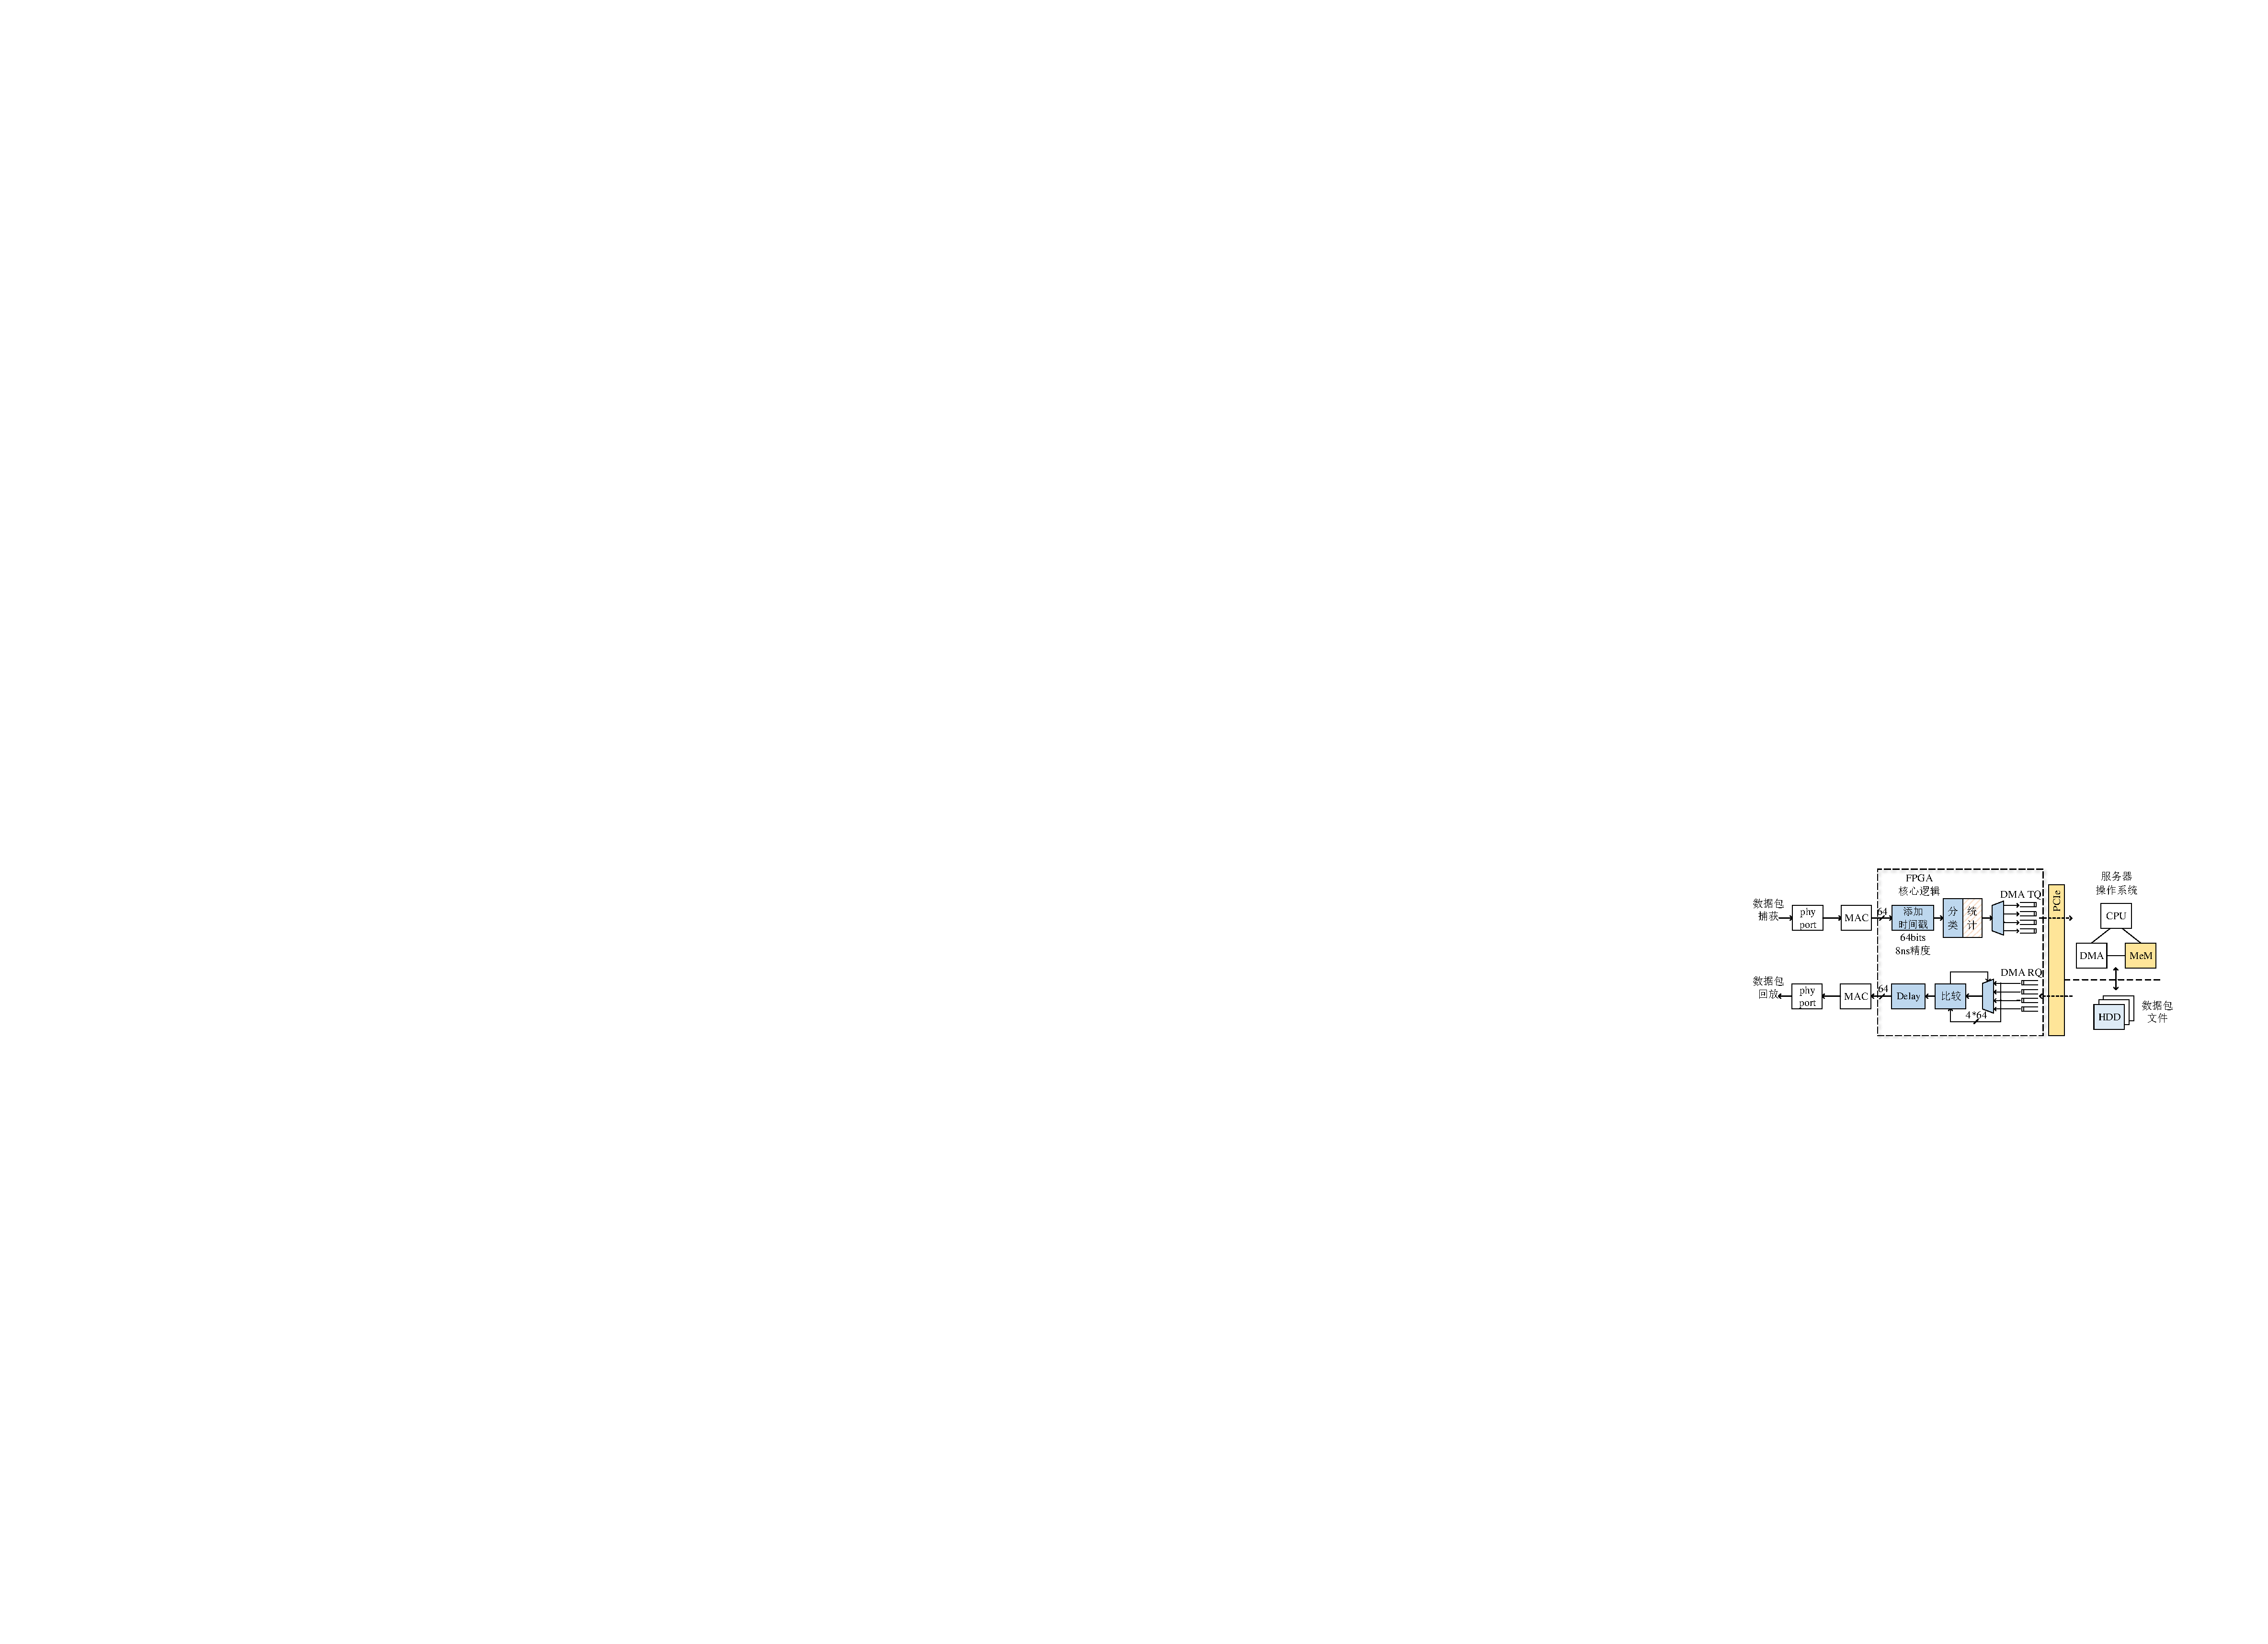
\includegraphics[scale=1]{arccaprep.pdf}
	\caption{流量捕获与回放系统数据通路FPGA核心逻辑架构} \label{fig:arccaprep}
\end{figure}

2)流量捕获---数据包处理通路。

在数据通路中,本文需要增添三个硬件模块:时间戳模块、流量均衡分类器和多路输出调度器。

\begin{itemize}
	\item 时间戳模块。为每个到达的数据包添加实时的64bit时间,数据总线结构如图\ref{fig:pktstruct}所示。FPGA数据通路主频为125MHz,每个时钟周期时长8ns。时间戳寄存器每个时钟周期都被触发一次自增8的加法操作。每个数据包到达有严格先后顺序,所以每个数据包的时间戳都是独一无二的。64bits数据可以表达正整数范围达到$1.8\times10^{19}$以上,从ns换算成年,相当于地球年的500年以上,数据位宽足够使用。
	\item 流量均衡分类器。流量捕获系统将数据包从网口传递到硬盘模组,整个链路中最有可能成为瓶颈的地方是硬盘的I/O驱动,由于普通机械硬盘真实外部读写性能只有1.5Gbps(SATA接口)左右\footnote{当时实验完成的板卡是以PCIe2.0$ \times $8为标准的主板插槽卡。互通总带宽为$ 5Gbps\times 8=40Gbps $,因而PCIe总线不是系统瓶颈。},这极大地限制了系统的性能。为了增大系统的最终捕获速度,本文将大流量通过硬件哈希算法分类为$N$条子流量。子流量的流速期望就变为之前总流量的$\dfrac{1}{N}$。哈希函数(CRC-16)的输入为网络流量数据包前五元组信息(目的IP地址,源IP地址,目的端口号,源端口号,协议标签)组成的104bits二进制数字。对于不包含五元组信息的数据包,可使用二层MAC地址(96bits)后补齐0,来组成新的104bits数字。CRC-16算法将输入数字转换成一组16bits的短数字,不同hash函数会转换出不同的值。但对于同一个hash函数不同的输入也可能得到相同的结果,最后我们选取结果的最后2bits位作为标记,以区分最终的缓存分支队列。一般的CRC函数都可以在同一个时钟周期内出结果,不会影响流水线性能。
	\item 多路输出调度器。多路调度器读取hash函数的输出结果并将此时的数据包按结果分发向不同队列。最终并行队列会分别上传到软件层,分别储存到不同的硬盘中。

\end{itemize}

\begin{figure}[!ht]
	\centering
	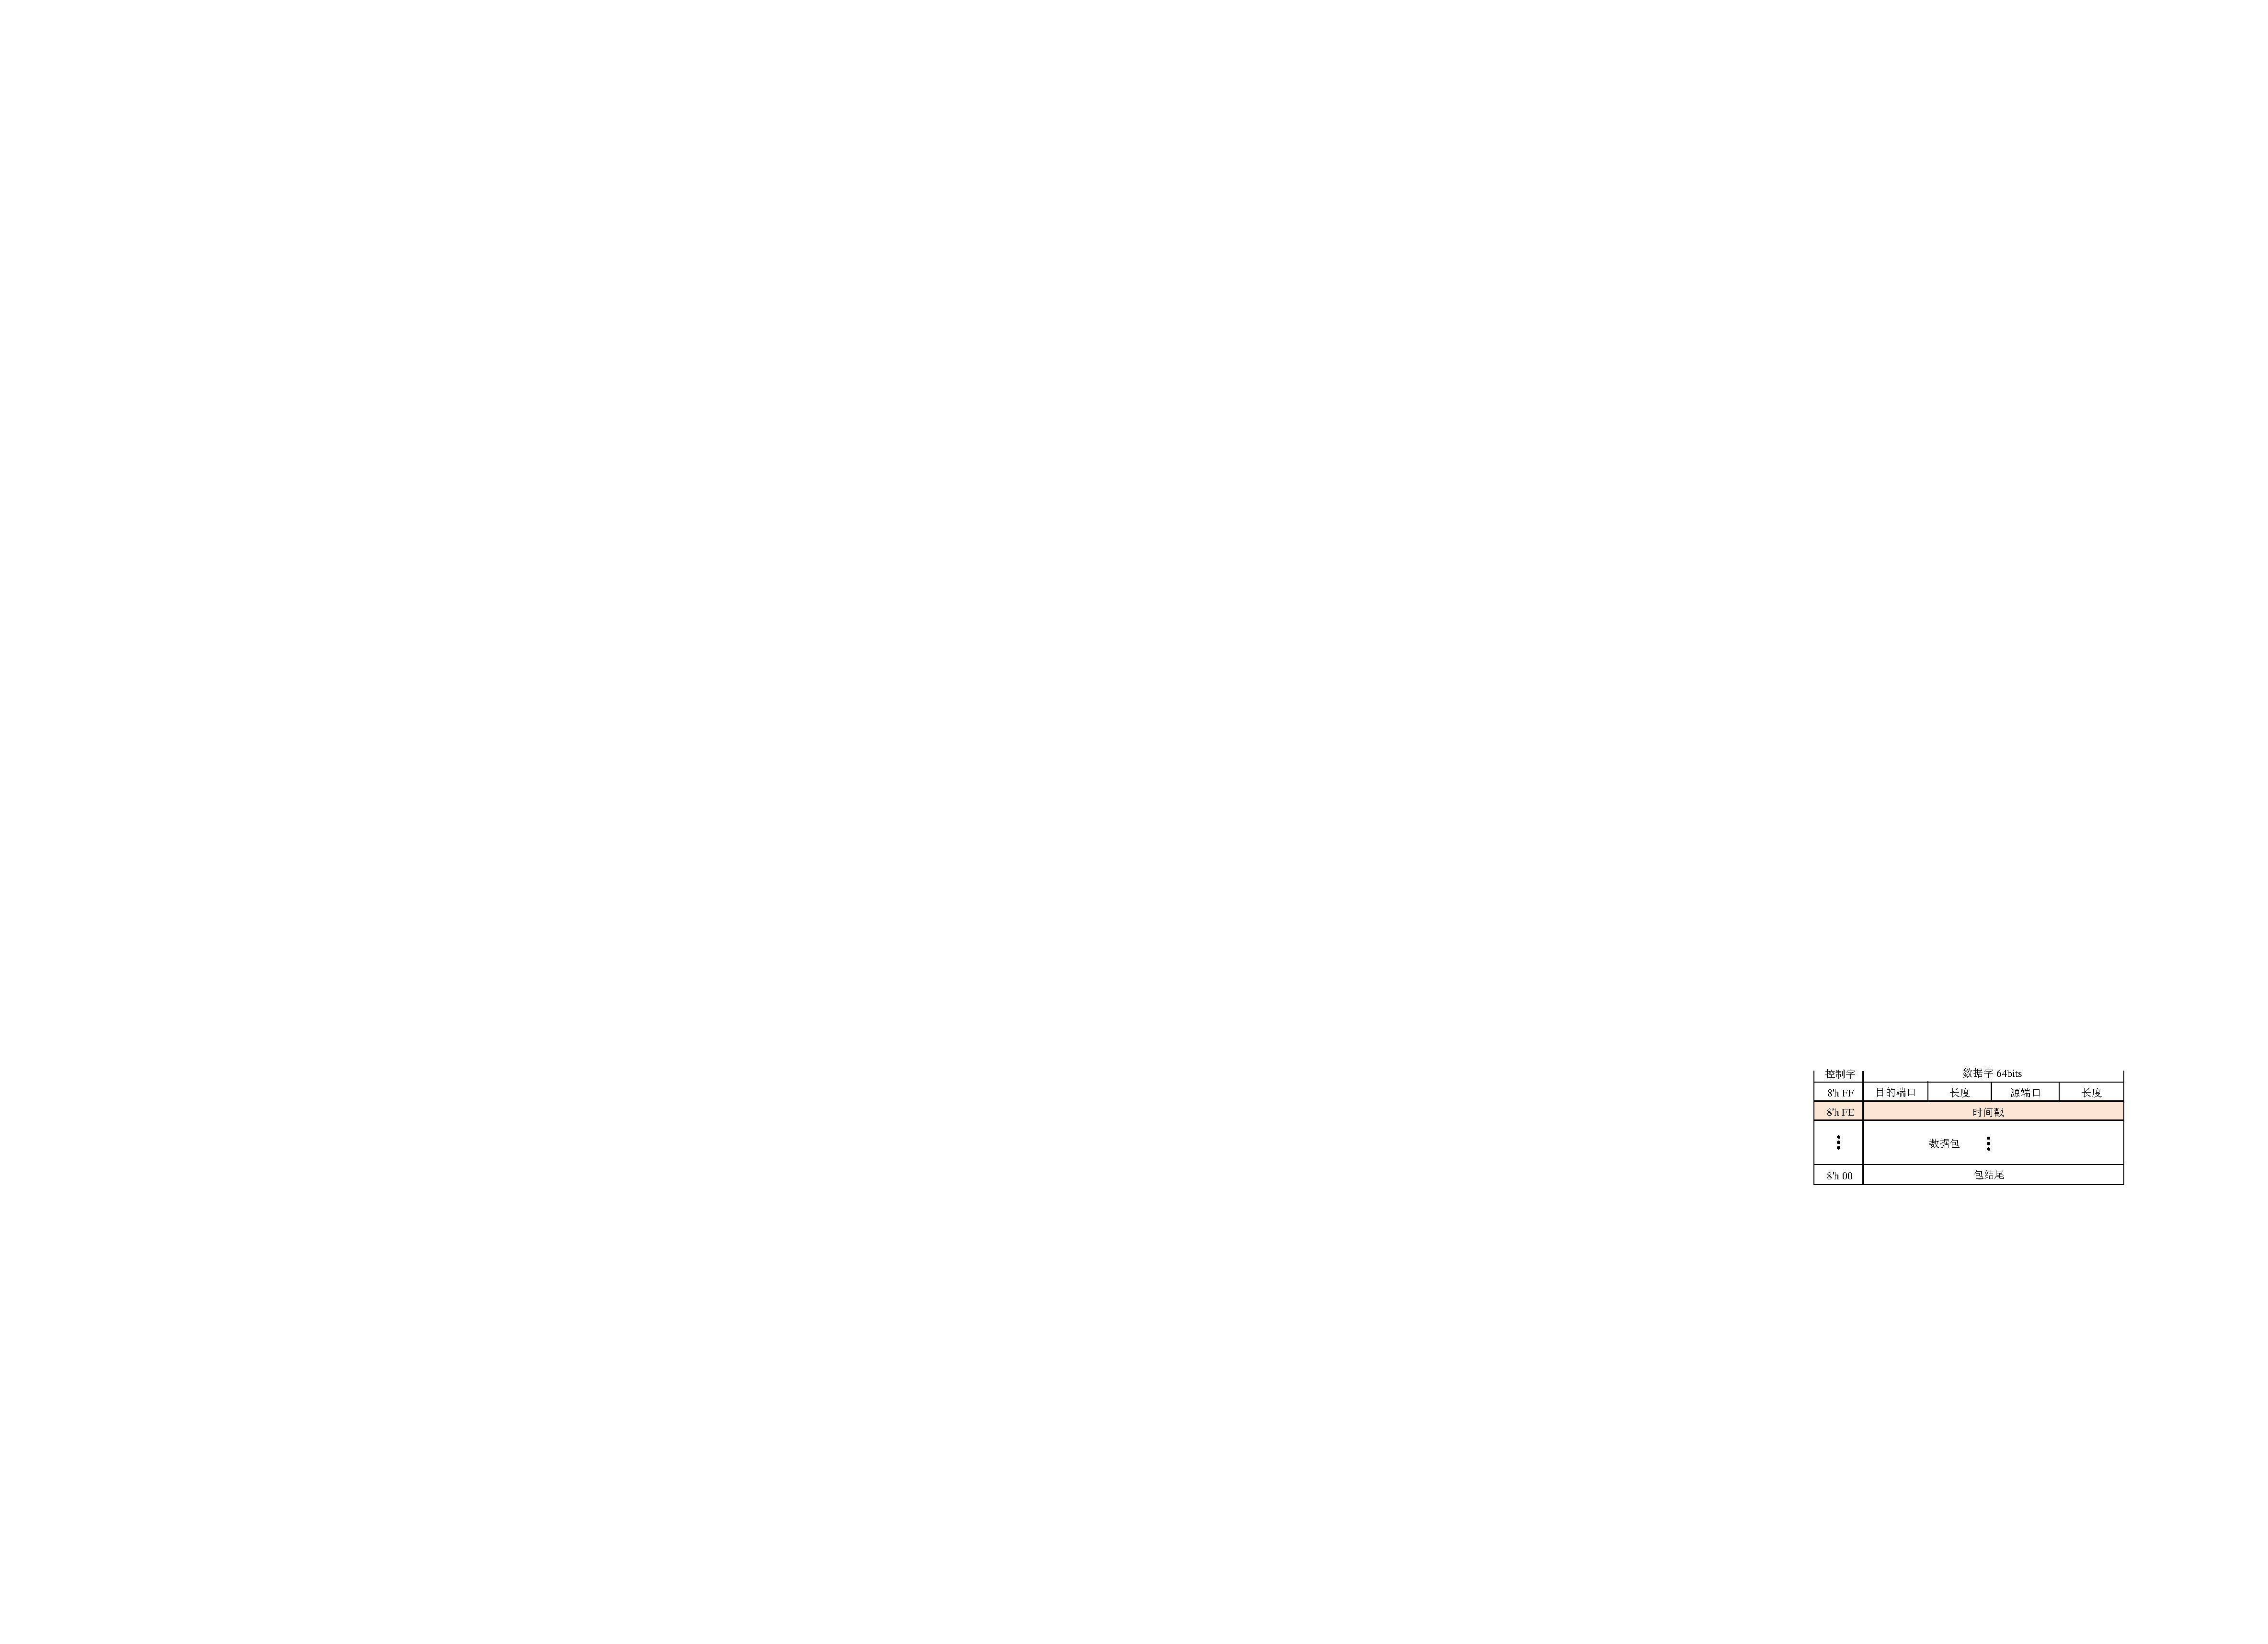
\includegraphics[scale=1]{pktstruct.pdf}
	\caption{数据包格式与控制字标志} \label{fig:pktstruct}
\end{figure}

3)流量回放---数据包处理通路。

流量回放是流表捕获的逆过程,数据从多列硬盘中读出并发送到FPGA内部多列缓存中。FPGA根据多队列数据流包头时间戳大小重新组合为一组数据流向板卡外发送,从而使系统可以完整模拟数据流现场状况。本文在回放通道中设计了两个硬件模块:时间比较模块、延迟开关。

\begin{itemize}
	\item 时间比较模块。此模块读取所有队列中的时间戳,并返回时间最小的时间戳所在的队列编号。在软件中,查找$N$个数据中的最小值时间复杂度为$ O(N) $。利用硬件逻辑天然的并行优势,可以对N组数据两两比较得出结果后,再对结果两两比较,这样只需要$ O(log N) $级比较即可输出最小值。值得注意的是,只有在比出最小值后取出队列首包,弹出后续包时间戳数据后,才能进行第二回合的比较。如果队列数过大,也许在同一个时钟周期内逻辑做不完比较儿产生输出不稳定的“竞争与险象”,从而得到错误的结果。例如,输入队列有64条,比较器的层数有6($ log_264 $)层,从中找出最小值需要至少2个周期或者3个周期时间\footnote{具体耗费时延与选用FPGA器件特性有关,例如更低nm制程响应速度越快,也与运行主频有关。}。如果查询时间超过一个时钟周期,数据在流水线中必然无法实现“背靠背”处理,总体处理流程都需要等待最耗时的这一级。
	\item 延迟开关。当选出最小时间戳的数据包后,并不是马上就可以发送出去,因为数据包与数据包之间有不固定的时间间隔。延迟开关的作用就是根据时间戳前后相对差值,让数据包等够所需的时间之后,再打开放行。这是提高数据包模拟真实环境相似程度的关键一步。
\end{itemize}

\BiSubsection{优化}{aa}

本小结主要分析流量捕获与回放系统的设计性能,并且探讨系统向目前主流网卡单网口100Gbps演进的优化方案。

上节提到,系统FPGA的主频选用125MHz,数据位宽64bits,则数据通路的总处理性能为$ P=8Gbps $。假设目标条件采集/回放速率$ T=4Gbps $,系统的瓶颈处:硬盘I/O需要扩充$ \dfrac{4}{1.5}=3 $倍,为保证性能可留有30\%的设计余地,则选取4块硬盘并行写入,总写入能力达到6Gbps。回放通路的逻辑瓶颈在于时间戳比较模块,4路数据可以在一个周期内比较完成,因而也满足处理性能大于实际需求。
由于当时技术协议发展水平受限,设计板卡的需求与现在相比略低。

如要适配当前高速率环境下的新协议,本文须重新分析设计瓶颈。FPGA内主要数据通路性能必须要大于100G(本文选取200MHz主频,512bits数据位宽),需要网卡拥有1路100G的网口,PCIe3.0$ \times $16($8Gbps\times 16=104Gbps$)的互通带宽。目前主流高性能固态硬盘的读写性能达到10Gbps,因此我们需要选择16路分流并行存储,来解决存储I/O瓶颈,至此捕获通路无性能瓶颈。回放通路的性能瓶颈在于16个队列时间戳最小值比较,由于16队列需要至少4层并行2进1比较器,需要2个时钟周期才能完成。因此回放数据通路的处理性能只能达到100Mpps,但是这并不意味,处理性能也会下降一半(到50Gbps),只是在处理时无法满足最小包长的100G性能。如果通路内均为128字节包长,则系统也可达到100G线速。由于真实网络环境的平均包长度为600字节,留给每个数据包10个时钟周期的处理时间,因此在真实情况下性能是满足的。



\BiSection{统计---网络测量实时压缩}{aa} %4

\BiSubsection{概述}{aa}

随着云数据中心规模不断增长,基础设施架构自我设计制造成为主流,网络运营商因此有能力在网络监控和管理方面投入更多。目前许多基于云端和裸金属环境新提出的新应用(hypervisor,虚拟机管理)和算法(BBR,拥塞控制算法)对各种各样的网络测量结果产生极大的需求。网络测量是指在运行的网络中测量各种实时变动的状态参数,例如RTT、包数量、流容量大小、流容量速度、拥塞程度等。这里大部分参数都可用被动方式进行测量,即,对运行中网络不引入任何影响。被动测量对网络运营商是一种有效的工具,例如,网络计费、安全监控、流量调度等。被动测量的过程一般分为2部分:首先,测量装置收集网络中的信息(通常以数据包驱动计数);第二,软件代理定期收集测量结果,并汇报上层控制层。


为解决监测系统软件实现效率低下的问题,研究人员提出一类“高速---低速”混合存储器更新方案。首先将流维护在高速缓存中(SRAM),此时SRAM的为每条流开辟空间较小,当SRAM中某条流溢出时,将此计数器值更新到DDR中,并为SRAM中对应的计数器清零。此方法有效减缓了DRAM的更新次数。但是会引入读值速度慢,硬件电路结构设计复杂等问题。此外,有工作提出将多个DDR用于并行统计以减小读值复杂度。然而随着数据量的增大,固定长度位宽的计数器依然有很高的溢出风险。

核心网络中,流量在转发节点总吞吐可达到上百T,流量数目可达到上百万,而流量转发节点数量也成百上千。对于精细地流量统计任务,每秒钟的更新量可能会达到150亿次\footnote{以10Tbps容量,转发64字节数据包计算。},而因统计所耗费的存储空间需求可以达到数百兆\footnote{以10M条流量,每条流统计占用8字节宽度为例。}。因此软件代理不可能做到每包更新。因而大量的统计数据缓存在本地高速内存中。
如此庞大的统计任务一般会由分布式设备进行加速以及分流统计。尤其在数据中心网络,服务器的数量众多,因此在流量的端处进行统计能够尽量减少计算存储和汇报的性能压力。

上一章提到,云计算网络的设计理念为尽可能降低服务器CPU因网络任务而带来的大量消耗。由于网络任务本身是以数据包为驱动的,在大型数据中心的服务器往往对外网络性能可达到100G,数据包触发速度可达到150Mpps。网络功能每增加一步操作都会引起数量庞大的额外计算。此外,统计功能所占用的大量存储空间也成为设计挑战。CPU中的一二三级缓存(cache)虽然速度极快,但容量相对较小(1MB以内)。则等待更新值的存储位置必然须在大容量的外置存储器(DDR)中,DDR的随机读写性能极低,面对如此高频度的更新需求,系统I/O带宽成为瓶颈。即使都将数据暂存于快速cache中,以目前主流服务器CPU的2.5GHz左右时钟频率估计,更新频率大概也只有主频的十分之一或百分之一。两种因素互相钳制,导致使用主机CPU做细粒度统计开销极大,在CPU时间成本极大的云服务器领域,测量的效率问题成为亟待解决的一个难点。

%这里做个表,说明一下问题的几个要点。。。。乔思祎2020年7月10日21:46:17
\BiSubsection{问题分析}{aa}

被动测量在网络中是一种基础服务,尤其在拥有可编程智能网卡的大型数据中心内,为实现高性能测量提供了可行性。目前FGPA板载高性能存储容量都有几十MB,为实现各种应用提供了丰富的逻辑资源。然而如果将所有测量项目都实现在硬件中,依然会造成片上资源过度消耗。一方面,如果更产生一种新的测量需求,就重新开发硬件逻辑,这会对网络操作人员造成严重的时间浪费。另一方面,因为FPGA其他逻辑资源也需要消耗一定数量的存储,各个逻辑模块需要均衡地使用存储资源。为了FPGA后期布局布线,板载资源使用率尽量小于全部资源的70\%。这为本文研究基于FPGA的测量技术带来了极大挑战。

本文基于一种在硬件中实现的可压缩每流测量算法,有效地解决了此问题,从而可以在硬件上为每一条流保持统计信息,并且只使用少量的存储资源。即使使用大存储容量的器件,如果在实际应用中不使之压缩,统计学上总有计数器值溢出的风险。

\BiSubsection{基于硬件设计压缩效果与问题}{aa}

1)压缩算法

目前基于抽样的压缩统计方法是一种新兴的测量设计思想,因为只须将一部分数据包被选中而送往统计模块,这样可以大大降低存储资源消耗,同时能够减少计数器累加次数。简单抽样对于均匀流量有很好的效果,但是对于各个流量大小不一的场景,小流的误差值会很高。现阶段各类抽样方法中可被证明拥有最佳估计误差的压缩算法是DISCO算法。%加引用 乔思祎2020年7月11日11:06:36
DISCO算法是一种可被证明的无偏估计压缩方法,DISCO算法的核心目标是减少高速缓存内关于每条流计数器的位宽占用大小,并且对包个数以及字节数的压缩都可适用。

假设$ c $是计数器中存储的值(被压缩后的),$ n $为统计流量大小的真实值,令函数$ n=f(c) $表示二者的压缩数量关系,

\begin{equation} \label{discofunc}
f(c)=\frac{b^c-1}{b-1}
\end{equation}

式中,$ b>1 $,且$ b $为系统预先设置的固定值。可发现,$ c=f^{-1}(n) $为一个凸函数,统计数值c的增长趋势一定是亚线性的。随着$ c $增大,$ f(c) $可近似为一个指数函数。因此对于一个足够大的$ n $,函数$ f(\cdot) $可将原来线性增加的数值压缩至$ O(log~n) $。每当长度为$ l $的数据包到达系统,针对此数据包的计数器应增加$ \Delta(c,l) $,此时$ c $为当前计数器压缩后的值。根据定义$ f(c) $,可以得到$ \Delta(c,l)=f^{-1}(l+f(c))-c $。如果存储$ c $的计数器采用浮点数计数,则每次对$ c $算出新增$ \Delta(c,l) $并相加后,得到的c都可以无误差地表达$ n $的真实值。但存储带小数位的浮点数会会占用更多存储空间,为了提高存储效率,须假定$ c $是一个正整数。



\begin{algorithm}[ht]
	\caption{DISCO算法计数器估计更新方法 \label{discoa1}}
	\IncMargin{2em}
	\DontPrintSemicolon
%	\KwIn{$\mbf{x}(k), \quad \mu, \quad \mbf{w}(0)$}
%	\KwOut{$y(k), \quad \varepsilon(k)$}
	%
	$ v = random(0,1) $
	
	分别计算$ \delta(c,l) $和$ p_d(c,l) $
	
%	\For{$k=0,1,\cdots$}{
%		$y(k) = \mbf{w}^H(k)\mbf{x}(k)$ \tcp*{output signal}
%		$\varepsilon(k) = d(k)-y(k)$ \tcp*{error signal}
%		$\mbf{w}(k+1) = \mbf{w}(k)+\mu\varepsilon^{\ast}(k)\mbf{x}(k)$ \tcp*{weight vector update}
%	}

	\eIf{$ v \leq  p_d(c,l)  $}
	{$ c = c + \delta(c,l) +1 $ \tcp*{显然,当$ p_d $越大,$ c $最终向上取整的概率也越大}}
	{$ c = c + \delta(c,l) $ \tcp*{向下取整}}
\end{algorithm}

DISCO算法为努力将存储空间降低,引入了一种概率估计。由算法\ref{discoa1},系统可以获取整数估计后的压缩值$c$。其中$ \delta(c,l) $和$ p_d(c,l) $由下列公式定义:

\begin{equation} \label{discofun2}
\delta(c,l)=\lceil f^{-1}(l+f(c)) - c \rceil - 1
\end{equation}

\begin{equation} \label{discofun3}
p_d(c,l) = \dfrac{l+f(c)-f(c+\delta(c,l))}{f(c+\delta(c,l)+1)-f(c+\delta(c,l))}
\end{equation}

经一段时间的统计,监测设备向控制器上报计数值$ c $,控制器可由公式\ref{discofunc}快速反向推导而出,同时此估计方法的无偏性由论文\citeup{hu2013discount}给出。

%\begin{equation} \label{discofun4}
%e \leq \sqrt{\dfrac{b-1}{2}}
%\end{equation}

2)压缩算法硬件实现的效果

算法\ref{discoa1}中,除加减法与比较、判断之外,求函数$ f(\cdot)$与$ f^{-1}(\cdot) $的关键计算指令是求“指数”与“对数”。 计算机快速计算指数,一般使用自然底数变换法,辅以查询算数表以及对精度的层层消除,计算时间由原来硬解法的$ O(n) $,降低至20个指令周期左右。对数函数可以使用泰勒级数展开来近似计算,展开后计算方法均为指数乘法和加法,进而再次转化为指数复杂度的计算。

DISCO算法提出后,由软件实现并达到单CPU核心11Gbps处理能力。目前的服务器终端网络通信容量已由40Gbps向100Gbps发展,继续扩展CPU核数满足处理需求已显低效。网络通信包数据量巨大,即使使用快速算法也无法满足网卡的线速处理需求。100G网卡的数据包处理速度需求为大约150Mpps,数据通路内时钟主频不会超过300MHz。按上限计算,每个数据包的处理时间余量只有2个时钟周期(与快速算法相比,本文需求超过其能力1到2个数量级)。当然流水线设计方法可以把计算过程拉长到多节拍,从而保证吞吐量。但需要注意,本算法中数值$ c $有先后依赖关系。即,首包处理时,$ c $若没有完成更新,第二个数据包无法进入处理通道。因此从全局看,更新环节无法真正打开为多级流水线。

注意到,本文公式中所有的底数b为预先确定值,因此在实践中可以存储只关于b的计算表,这样可以最大限度减小计算复杂度,也比较节约计算用存储资源。假定计算表的深度为3072,宽度为32bits,选定$ b=1.006 $。系统支持的最大计数量等效于$ f(3072)=1.59\times10^{10}Bytes=15GB $。而计数器$ c $只需要12位(保存压缩后的值,$ 2^{12}=4096 $),而在不压缩的线性计数下则需要至少34bits的存储位宽($ 2^{34}=1.71\times10^{10}>1.59\times10^{10}$)。即,对于指数计算需求$b^X (X \leq 3072)$,系统可以通过单周期查表方法获取结果。


使用查表法加速指数计算可获得很好的效果,但对数计算($ log(X) $)即指数反函数计算无法实现一周期出结果。对数计算一般反向利用指数表进行二分估计。如图\ref{fig:logsearch}所示,左边为上述的指数预计算查找表。初始化值,c=0,f(c)=0,假设此时到来数据包长度为1500字节。根据公式\ref{discofun2}计算$ \delta(c,l)$,以及公式\ref{discofun3}计算$p_d(c,l) $。首先,在计算$ \delta(c,l)$时,最关键需要计算 $ f^{-1}(l+f(c)) $,带入$ l=1500 $、 $ f(0)=0 $,得到:

\begin{equation} \label{discofun4}
f^{-1}(1500+0) = x \rightarrow f(x)=1500 = \dfrac{b^x-1}{b-1}
\end{equation}

带入b=1.006,经过变换:

\begin{equation} \label{discofun5}
b^x=1500\times(b-1)+1\\
= 1500\times 0.006+1\\
=10
\end{equation}

因此,计算$ f^{-1}(1500+0) $的结果可以等价为:在指数计算表中查找当$ x $等于多少时指数值为10。由于指数值是非连续、非等差数列,查找方法只能使用二分法逼近。如图\ref{fig:logsearch}右侧所示,在3072个表项中从第一行开始进行二分查找至少需要12次跳转。

\begin{figure}[!ht]
	\centering
	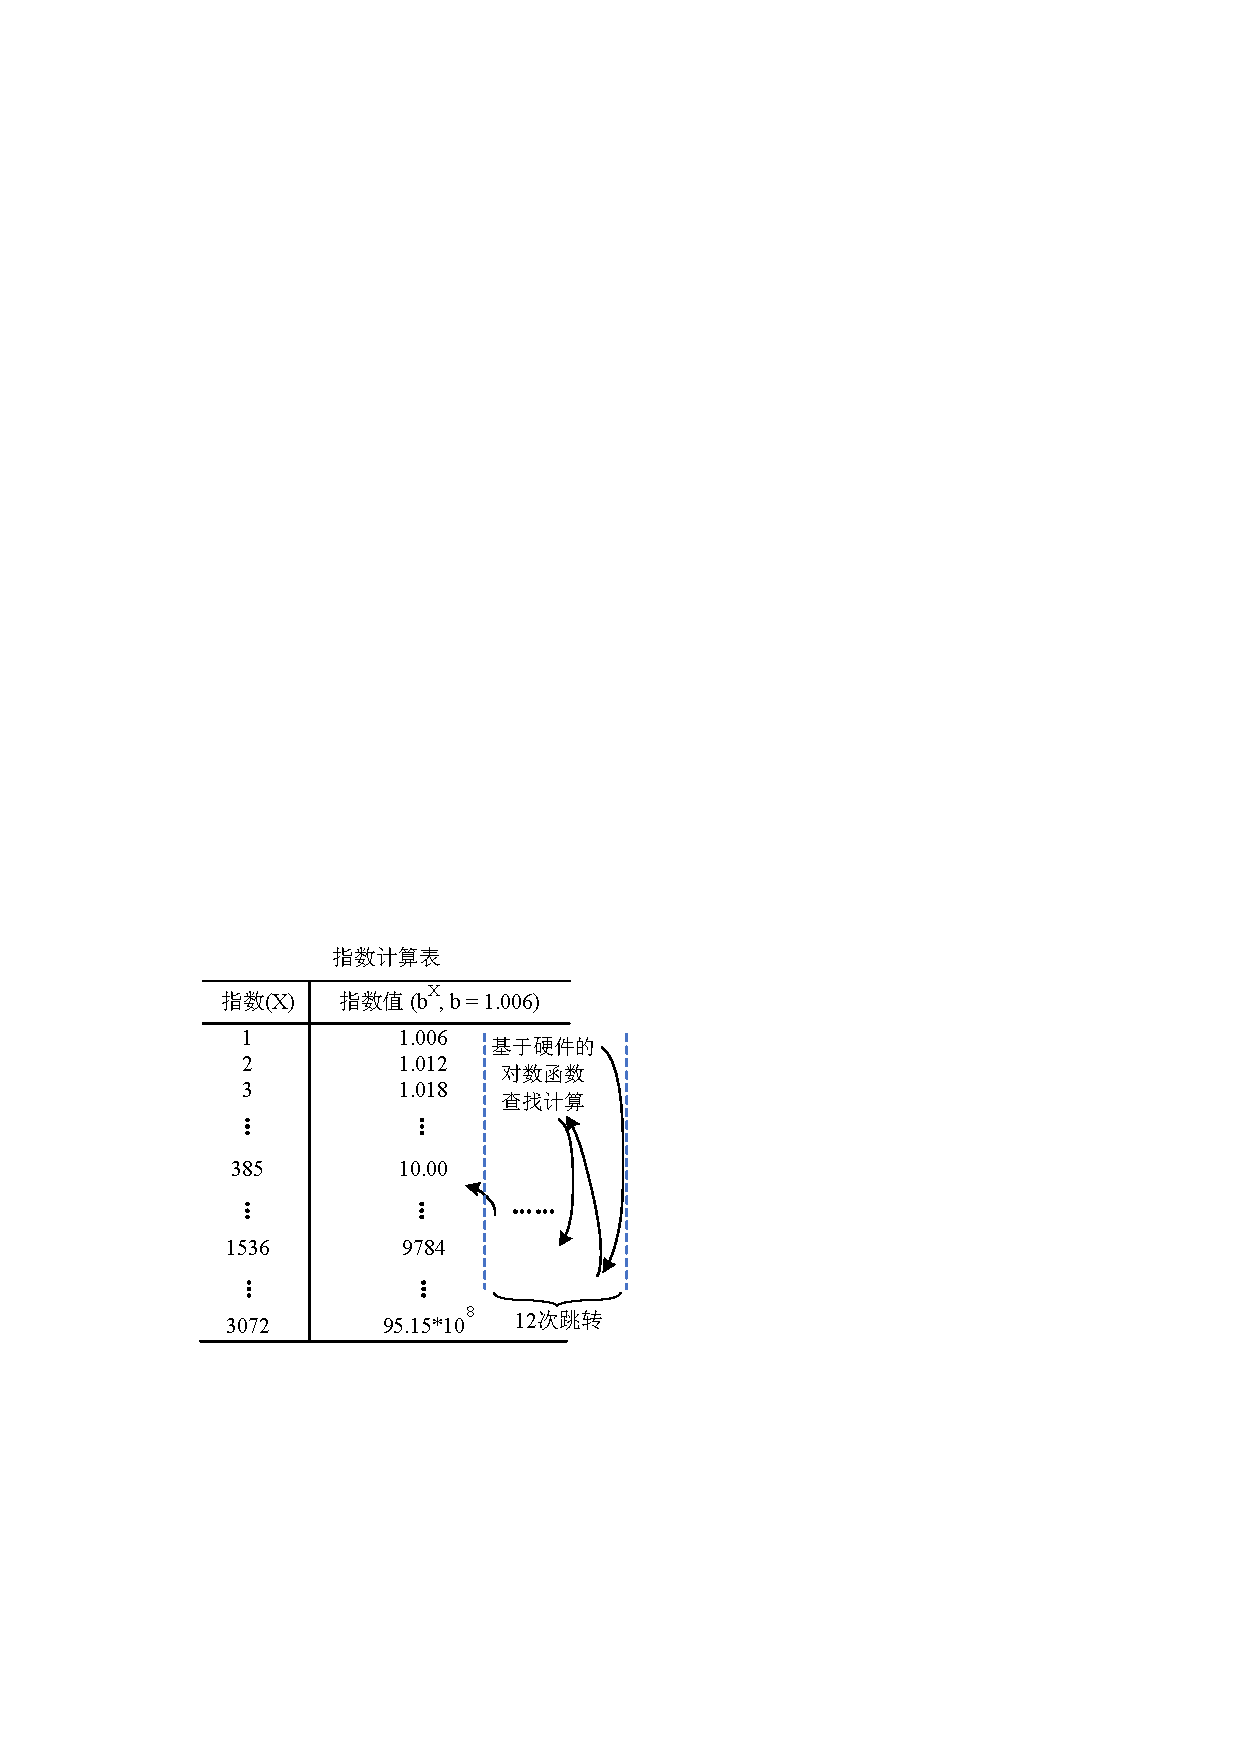
\includegraphics[scale=1]{logsearch.pdf}
	\caption{反向利用指数表进行二分估以计求得对数函数值} \label{fig:logsearch}
\end{figure}

计算出$ \delta(c,l)$后,$p_d(c,l) $可由指数查表与$ \delta(c,l)$结果共同计算。本文发现,由于不同的$ c $数值与不同$ l $数值,基于硬件计算$ \delta(c,l)$的时钟周期并不固定,例如当前c=1536,那么对数查找的起始位置便不在第一行,而在整体表的中间位置,这样搜索空间会缩小,因此查找次数也会变少。如图\ref{fig:searchtime}所示,假设流每个数据包大小统一为$ l=1000 $,当c的值越来越大,查找次数会往减小的趋势发展。

\begin{figure}[!ht]
	\centering
	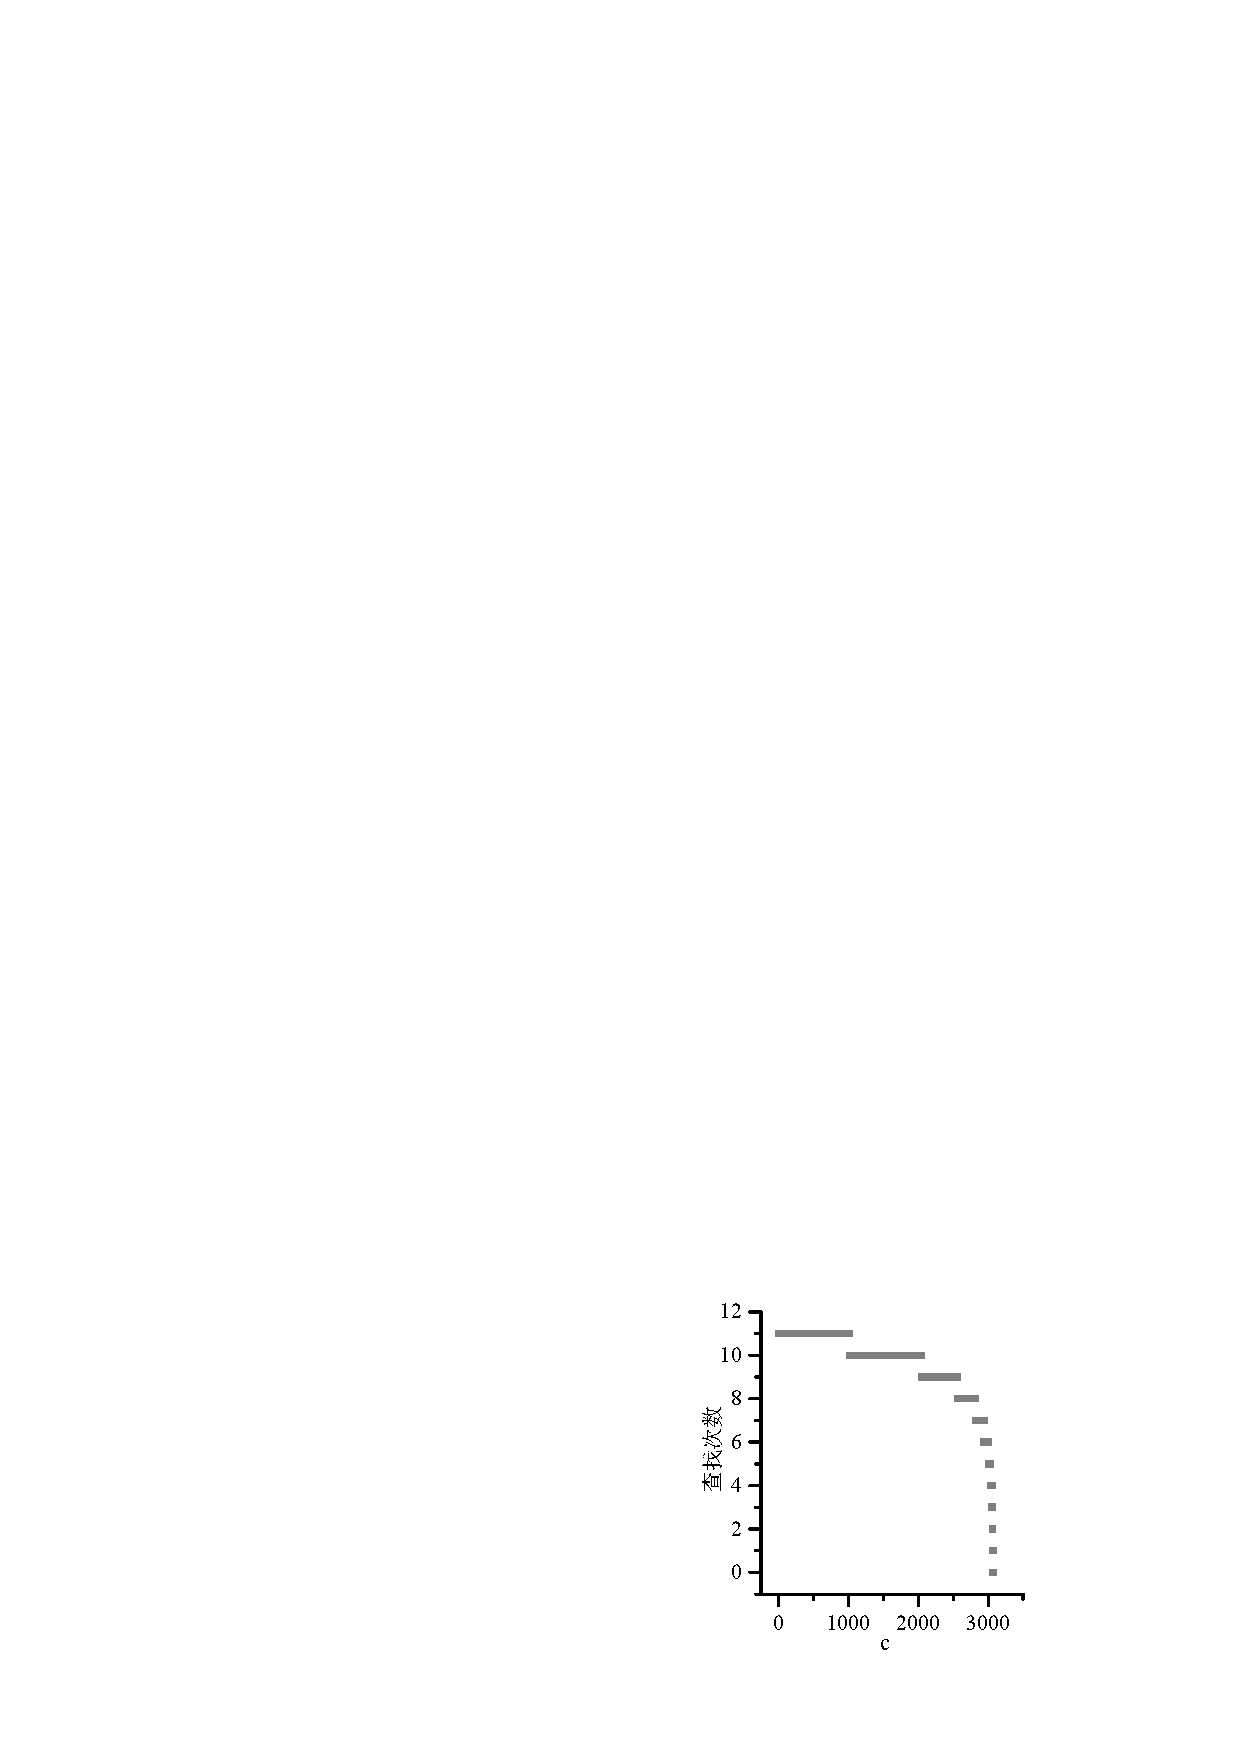
\includegraphics[scale=1]{searchtime.pdf}
	\caption{当流量中包长$l=1000$时利用指数表求对数函数值的查找次数} \label{fig:searchtime}
\end{figure}



3)存在问题。

\begin{figure}[!ht]
	\centering
	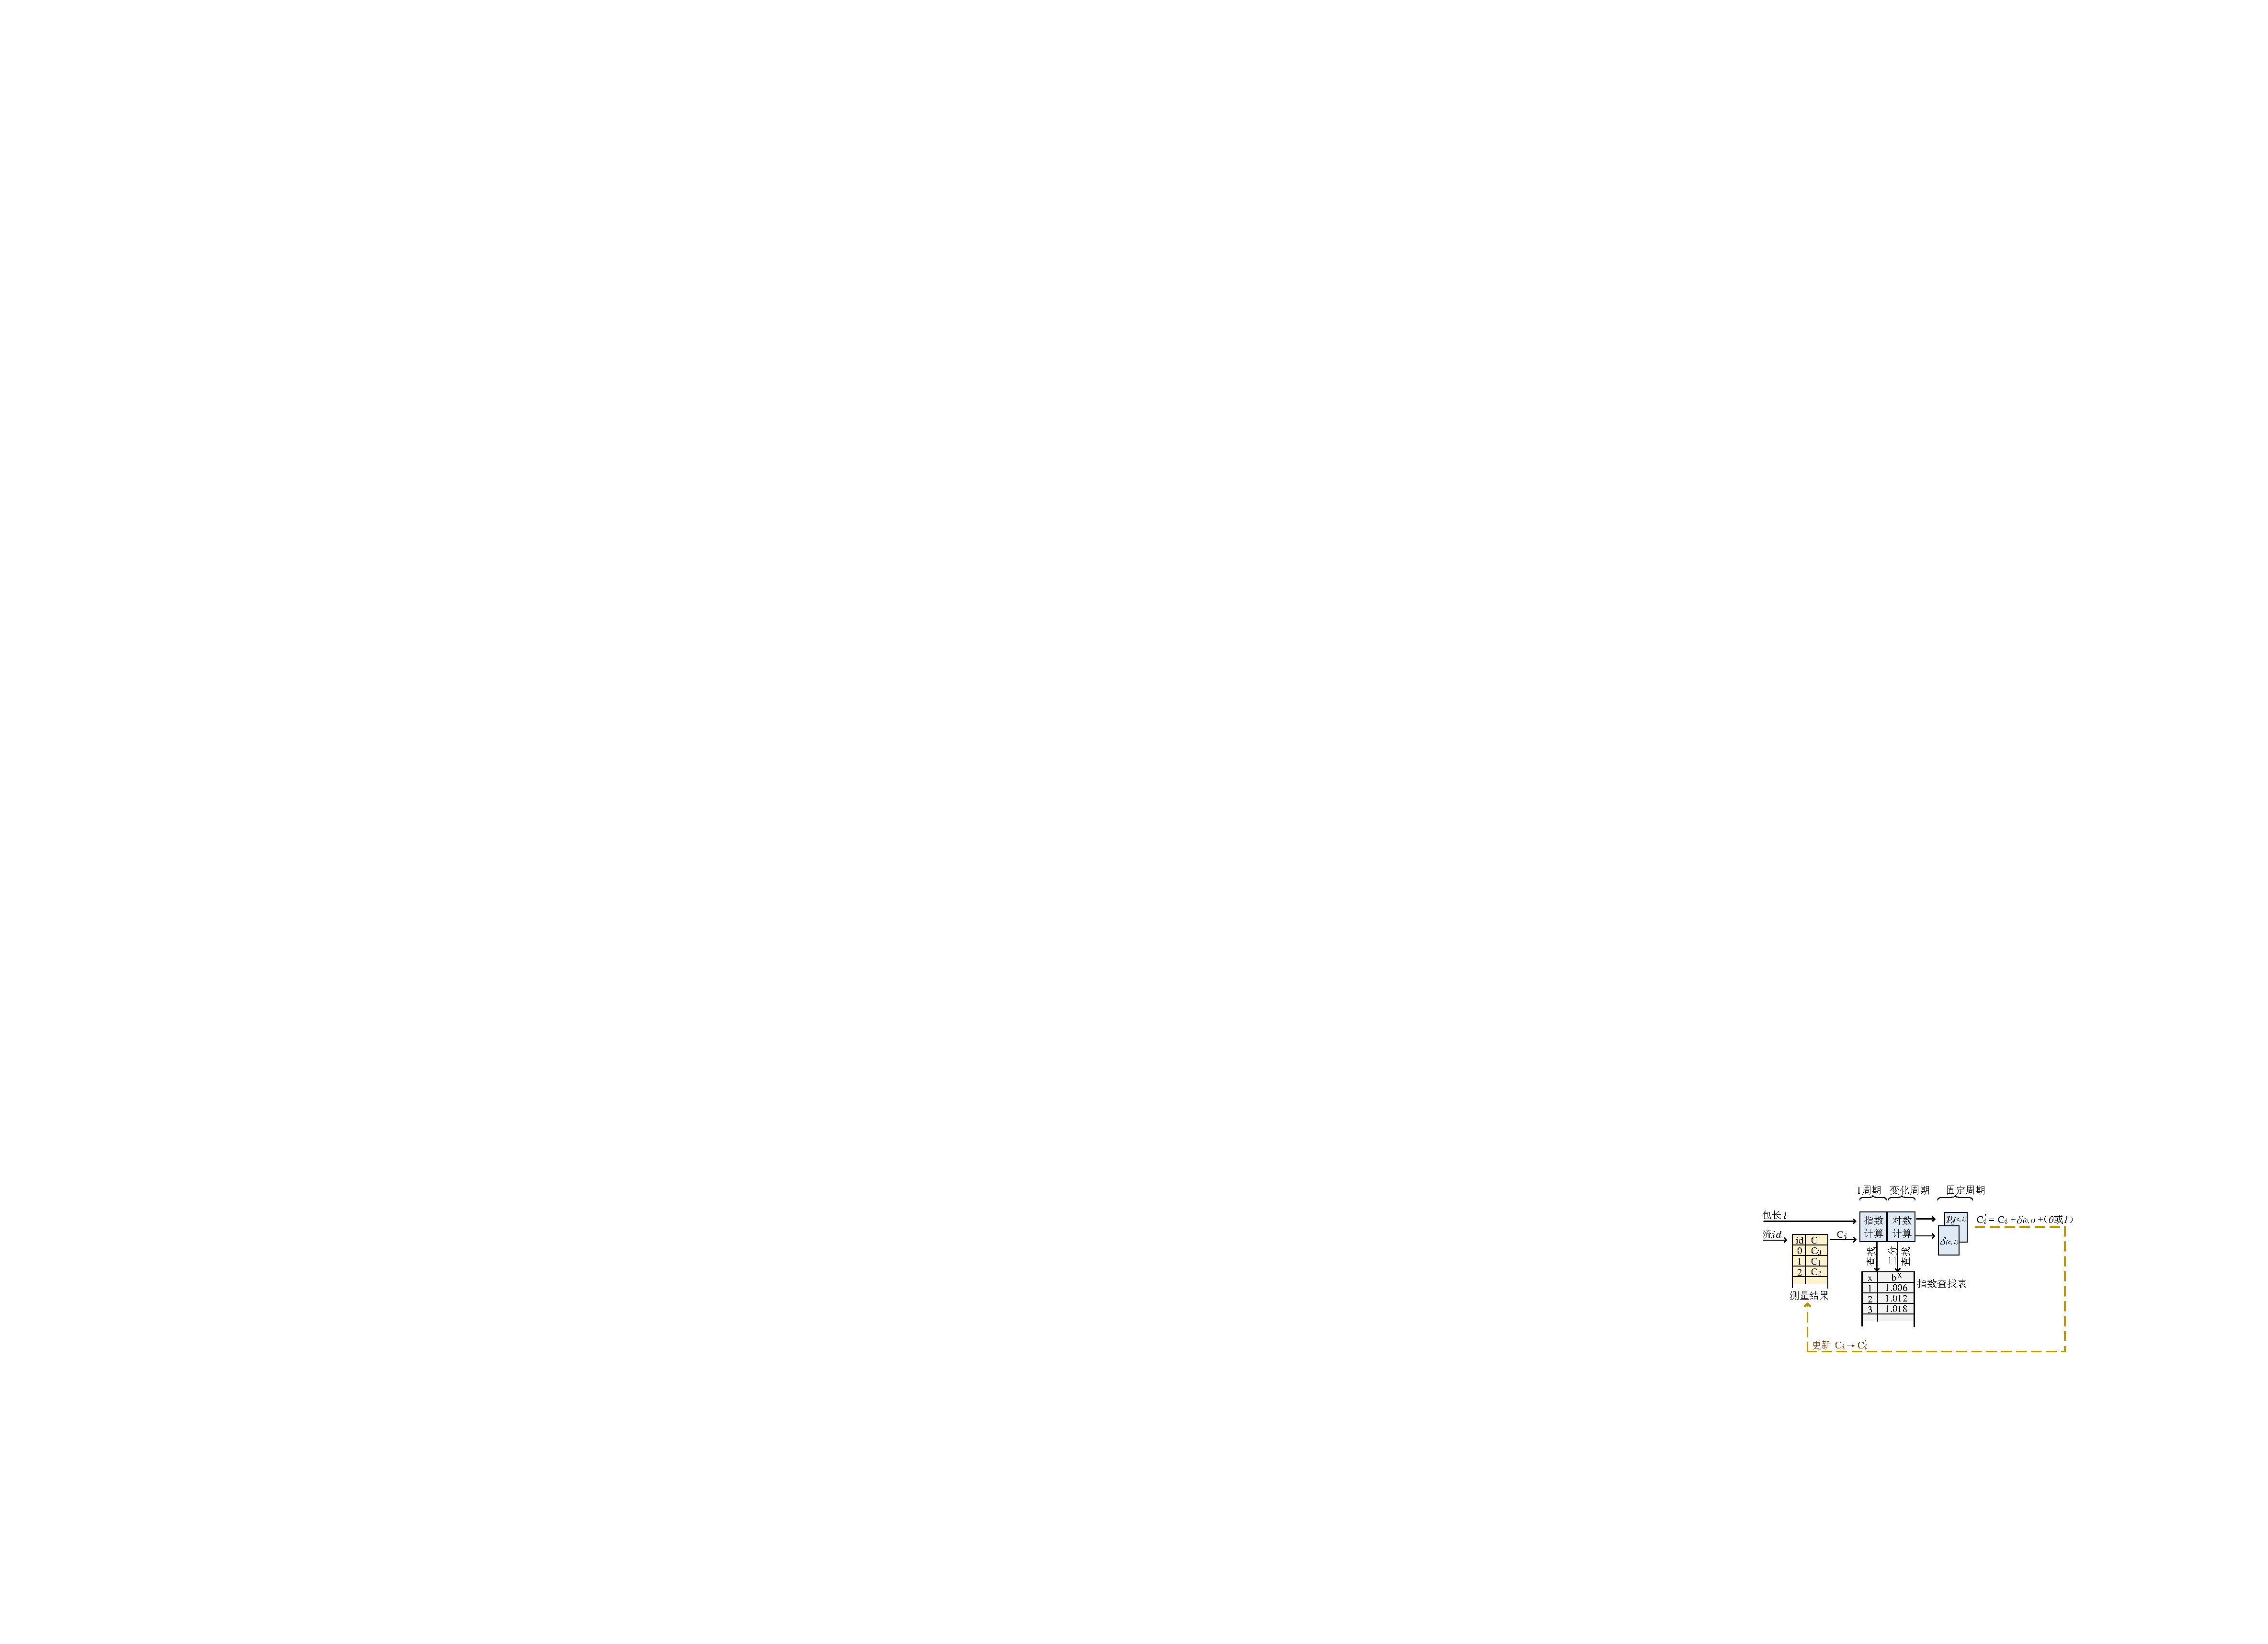
\includegraphics[scale=1]{originpipeline.pdf}
	\caption{压缩统计硬件流水线设计(未优化)} \label{fig:originpipeline}
\end{figure}

本文总结上述分析,并将基于软件的DISCO算法硬件流水线在图\ref{fig:originpipeline}中展示。当数据包到达系统,首先获取当前对应流的统计量$ C_i $,之后由指数计算和对数计算模块求出中间变量,最后通过四则运算得到关键判定值$ \delta(c,l)$和$p_d(c,l) $。对其进行性能分析:硬件设计为提高吞吐量一般采用流水线设计。为统合前后分级的节拍,要求每一级流水线的时延固定。本文发现二分查找虽然平均时延只有7周期,但最长时延可达到12周期,最短只需1周期,因此为了使流水线对外表现稳定,需要在硬件设计逻辑是增加许多配合打拍的逻辑,资源效率较低。另外在计算关键判定值时需要使用两次除法器。逻辑除法在FPGA设计中一般耗时需要40个周期以上,虽然除法器可以以流水线方式工作以提高吞吐,但本算法有一个更新闭环,在只有一条流量的时候,前后两次更新时间内不可进入流水线计算。
因此一次更新所耗费的时长大约为50个周期,假设FPGA数据通路主频是300MHz,因而更新频率只有6Mpps。若对应64字节最小包,硬件加速后也只能达到4Gbps线速,与本文100Gbps设计目标相差甚远。

\BiSubsection{优化}{aa}

1)符合DC抽象的算法优化方法

前文提到的优化设计方法原则1:每一级有应有固定的节拍数。因为更新压缩表有强烈前后依赖关系,因此找到如何缩短整体处理时间,以及将可变动节拍计算逻辑固定化(应向减少节拍的方向优化)是本文的重大挑战。

本文发现,若$ c $值处于比较大的阶段,当进行每包更新时,$ c $与更新值$ c' $的差值最大为1。即,公式\ref{discofun2}中$ \delta(c,l)=0$。因此,根据算法\ref{discoa1},有:

\begin{equation} \label{mydiscof1}
c'=c+\delta(c,l) + 1 =c+1
\end{equation}

这是一个很重要的现象,由前一节本文提到,若想加速环节内的计算速度,须减少更新循环内耗费的时钟周期数。则要将时序数可变的逻辑修正为固定时序逻辑,且应该尽量朝向能够减小时钟周期占数的方向。如果只需要判断c更新后的值加一与否,也许可以避免掉大量的对数二分查找过程。另外对于当c比较小的时候,本文将其计数转化为线性增加,因此计算复杂度也很低,若c较小也表明占用的计数位宽度不会很大。接下来本文分析此方案的可行性。本文首先分析,当$ \delta(c,l)=0$时系统状态。由公式\ref{discofun2}与\ref{discofun3},本文得到:

\begin{align}
\delta(c,l) =  \lceil f^{-1}(l+f(c)) - c \rceil -1 &= 0 \nonumber \\
\lceil f^{-1}(l+f(c)) - c \rceil &= 1 %\\
%\lceil f^{-1}(l+f(c)) - f^{-1}(f(c)) \rceil &= 1 
\end{align}

因此,得到:


\begin{align}
0 &\leq f^{-1}(l+f(c)) - c \leq 1 \nonumber  \\
0 &\leq f^{-1}(l+f(c)) - f^{-1}(f(c)) \leq 1
%\lceil f^{-1}(l+f(c)) - f^{-1}(f(c)) \rceil &= 1 
\end{align}

%\begin{equation} \label{mydiscof1}
%
%\end{equation}

由于$f^{-1}(\cdot)$是增函数,且$l>0$,显然上述公式为正值,因此上述公式可变为:

%\begin{equation} \label{mydiscof2}
%f^{-1}(l+f(c)) - f^{-1}(f(c)) \leq 1
%\end{equation}

\begin{align}\label{mydiscof2}
f^{-1}(l+f(c)) - f^{-1}(f(c)) &\leq 1 \nonumber  \\
f^{-1}(l+f(c)) - c &\leq 1 \nonumber  \\
f^{-1}(l+f(c))  &\leq c + 1  \nonumber \\
l+f(c) &\leq f(c+1) \nonumber  \\
f(c+1) - f(c) &\geq l
\end{align}

在以太网规范中,包长$l \in [64,1518]$,根据上述不等式可知:须满足左边大于1518则不等式恒成立:

\begin{equation} \label{mydiscof3}
f(c+1) - f(c) \geq 1518
\end{equation}

由于$ f(\cdot) $是增函数且导数始终大于零,则一定可找到一个最小的$ c_{lmin} $值,满足:对于任意$ c \geq c_{lmin} $ 时,均有上式(\ref{mydiscof3})成立,也即$\delta(c,l) =0$。

下面关注此条件下$ p_d(c,l) $的计算过程,DISCO算法\ref{discoa1}对$ p_d(c,l) $的描述为:系统对压缩计数器以概率$p= p_d(c,l) $增加$\delta(c,l) +1$,以概率$p=1- p_d(c,l) $增加$\delta(c,l)$。由上文,因$ \delta(c,l)=0$,则此阶段的更新算法为:系统对压缩计数器以概率$p= p_d(c,l) $增加$1$,以概率$p=1- p_d(c,l) $增加$0$。

由公式\ref{discofun3}、以及条件$ \delta(c,l)=0$,得到:

\begin{align}\label{mydiscof4}
p_d(c,l) &= \dfrac{l+f(c)-f(c+\delta(c,l))}{f(c+\delta(c,l)+1)-f(c+\delta(c,l))}  \nonumber \\
&= \dfrac{l+f(c)-f(c+0)}{f(c+0+1)-f(c+0)} \nonumber  \\
&= \dfrac{l}{f(c+1)-f(c)} 
\end{align}



观察上式,本文发现,当$ c \geq c_{lmin} $ ,DISCO的计算操作可化简为算法\ref{discoa2}:

\begin{algorithm}[ht]
	\caption{当$ c \geq c_{lmin} $时约化的压缩算法 \label{discoa2}}
	\IncMargin{2em}
	\DontPrintSemicolon
	%	\KwIn{$\mbf{x}(k), \quad \mu, \quad \mbf{w}(0)$}
	%	\KwOut{$y(k), \quad \varepsilon(k)$}
	%
	$ v = random(0,1) $

	$ p_d(c,l)=\dfrac{l}{f(c+1)-f(c)} $ \tcp*{计算概率值}
	
	\eIf{$ v \leq  p_d(c,l)  $}
	{$ c = c +  1 $ \tcp*{根据概率值,计数器只增加1}}
	{$ c = c   $ }
\end{algorithm}

\begin{algorithm}[ht]
	\caption{求解硬件压缩算法不同阶段判定标志位$c_{lmax}$  \label{mydiscoa2}}
	\IncMargin{2em}
	\DontPrintSemicolon
	\KwIn{$b$ - 函数$f(c)$中的预定义参数}
	\KwOut{$c_{lmax}$ - 基于硬件DISCO压缩算法中判断标志位}
	%
	$ 	PKT\_Length\_MAX = 1518 $
	
	$ c=0 $
	
	\While{True}{
		$ c++ $	
		
		$ f(c+1)=\dfrac{b^{c+1}-1}{b-1} $
		
		$ f(c)=\dfrac{b^{c}-1}{b-1} $
		
		\If{$ f(c+1)-f(c)\geq PKT\_Length\_MAX $}{
			$ c_{lmax} = c $
			
			\Return $ c_{lmax} $
		}
	}
	
\end{algorithm}

但此式中依然包含了硬件除法,由前文分析知,此步骤须耗费数十个时钟周期\footnote{根据不同结果保留精度以及除数被除数位宽需求,商用Xilinx除法器IP核须要耗费40到80个时钟周期不等。},因此本文将概率计算公式继续化简为查表算法。这将解决本文提出优化希望的第二个重点问题:计算依赖数据之间的时钟周期数量过大。

观察公式\ref{mydiscof4},简化后概率$ p_d() $与两个变量$ c,l $有关,且计算时只依赖于简单函数计算过程。$ c $的范围在$ [1,3072] $之间,$ l $的范围在$ [64,1518] $之间。因此c与l合成的总体表项有4百万个,总共需耗费片上存储空间约32Mb--128Mb\footnote{以8bits或32bits为结果存储位宽计算。}由于FPGA内高速片上存储资源相对较少,实验用ONetCard网卡只有16Mb,然而目前比较高端的FPGA片上存储也只有100Mb左右\citeup{alveou250}。设计过程中需要折中考虑资源占用与计算速度的互相矛盾的关系。显然查表占据了过多硬件资源,在工程实践上是不合理的。

接下来继续观察公式\ref{mydiscof4},可发现:

\begin{align}\label{mydiscof5}
p_d(c,l) &= \dfrac{l}{f(c+1)-f(c)}   \nonumber \\
&= \dfrac{1}{f(c+1)-f(c)} \times l 
\end{align}

上式表明,参数$ p_d(c,l) $可分解为两部分,第一部分只与$ c $相关,另外一部分是一个乘数系数$l$。因此,本文将查表过程分解为两步:第一步,根据参数c查找数值$ p_c= \dfrac{1}{f(c+1)-f(c)} $,本文称此查找表为PLUT($p_d$ Look Up Table);第二步,计算$ p_d = p_c \times l $从而得到所需概率$ p_d(c,l) $。

\begin{algorithm}[ht]
	\caption{求解快速概率计算PLUT查找表  \label{mydiscoa3}}
	\IncMargin{2em}
	\DontPrintSemicolon
	\KwIn{$b$ - 函数$f(c)$中的预定义参数; $c_{lmax}$}
	\KwOut{$PLUT$ -快速概率计算查找表}
	%
	$Depth = 3072 $ \tcp*{查找表最深为3K条表项}
	
	$ PLUT[3072] $
	
	\For{$c=c_{lmax}$ , $c_{lmax}+1$ , $\cdots$,$ Depth $}{
		
		$ f(c+1)=\dfrac{b^{c+1}-1}{b-1} $
		
		$ f(c)=\dfrac{b^{c}-1}{b-1} $
		
		$ 	p_c=\dfrac{1}{f(c+1)-f(c)}\times 2^{21.4} $
		
		$ PLUT[c] = p_c $ \tcp*{保存表项内容}
	}
\end{algorithm}



系统在初始化之前须计算PLUT表项中的值。概率值是一个归一化的数值,但在硬件中浮点数的处理比较复杂且存储效率低。本文将概率归一化为32bits最大的整数值($2^{32}=4294967295$),因此$ p_c \times l  $不应超过 $ 2^{32} $,$ p_c $的最大值应满足$ l_{max} \times p_{cmax} = 2^{32 } $ ,得到:

\begin{equation} \label{mydiscof6}
p_{cmax} \leq \dfrac{2^{32}}{1518} =2829359.2=2^{21.4}
\end{equation}



因此硬件中除了一个深度为3k的PLUT表,还需要一个最大22bits$\times$12bits(PLUT$\times l$)的窄单周期乘法器\citeup{xilinxmulti}即可,最大总共消耗两周期即可完成所有计算。设计中的查找表占片上存储容量约9KB(=3K 深度$\times$3Bytes),远小于板上资源限制条件。

\begin{algorithm}[!h]
	\caption{硬件统计压缩算法(优化)  \label{mydiscoa4}}
	\IncMargin{2em}
	\DontPrintSemicolon
	\KwIn{$l$ - 每个到达数据包的待统计包长度;   $id$ - 每个数据包的流分类标号;  $ Counter\_Table[] $ - 统计计数器存储组; \\ \quad\quad\quad $c_{lmax}$ - 基于硬件DISCO压缩算法中判断标志位}
	\KwOut{完成快速更新统计表$ Counter\_Table[id] $}
	$f(c)=\dfrac{b^c-1}{b-1}$ \tcp*{初始化过程}
	
	$M\_Number = f(c_{lmax}) $ \tcp*{计算判断标志位所对应的统计容量}
	
	$ Counter\_Table[id] = 0 $ \tcp*{计数器初始值均为0}
	
	\tcp*{循环开始,针对每个到达数据包都做计算}
	\For{ Each incoming packet}{ 
		$ v = random(0, 2^{32}) $         \tcp*{获取一个随机数字,范围为0-4字节内任意数字}
		
		$ c_{current} = Counter\_Table[id] $
		
		
		\eIf{$ c_{current} + l \leq M\_Number $}{ 
			
			$ c' = c_{current} + l $ \tcp*{判断是否属于第一阶段,只进行线性统计并更新}
			
			$ Counter\_Table[id] = c' $
			
		}{	
			\eIf{first time get into $ 2^{nd} $ stage}{ 
				
				$ l = l - ( M\_Number - c_{current}) $ \tcp*{首次进入第二阶段须在存储数据的最左bit位增加标志位,并初始化}
				
				$ 	c_{current} = c_{current} \quad | \quad 22'b{10\_0000\_0000\_0000\_0000\_0000} $
				
				$ 	c_{current} = c_{current} \quad \& \quad 22'b{10\_0000\_0000\_0000\_0000\_0000} $
				
				$ p_c=PLUT[c_{lmax}] \times l $ 
				
				\eIf{$ v \leq p_c $}{
					
					$ 	c' = c_{lmax} + 1 $
					
					$ 	c_{current} = c_{current} \quad \&\quad c' 	 $
					
				}{
					$ 	c_{current} = c_{current} \quad \&\quad c_{lmax}	 $
				}
				$ Counter\_Table[id] = c_{current} $  \tcp*{第二阶段进行压缩统计并更新}
			}{
				
				$ c = c_{current} \quad \&\quad 22'b{01\_1111\_1111\_1111\_1111\_1111} $
				
				$ p_c = PLUT[c] \times l $
				
				\If{$ v \leq p_c $}{   
					$ 	c_{current} = c_{current} + 1 $ \tcp*{第二阶段为压缩计数阶段并进行更新}
					
					$ Counter\_Table[id] = c_{current} $
				}				
			}			
		}
	}
\end{algorithm}

本文给出对于任意的系统测量需求范围计算上文提到的$ c_{lmin} $(算法\ref{mydiscoa2})以及PLUT表(算法\ref{mydiscoa3})的计算方法。这两组参数均在系统初始化之前由控制器离线计算完成,在系统运行时加载如硬件查表空间即可。



\begin{figure}[!ht]
	\centering
	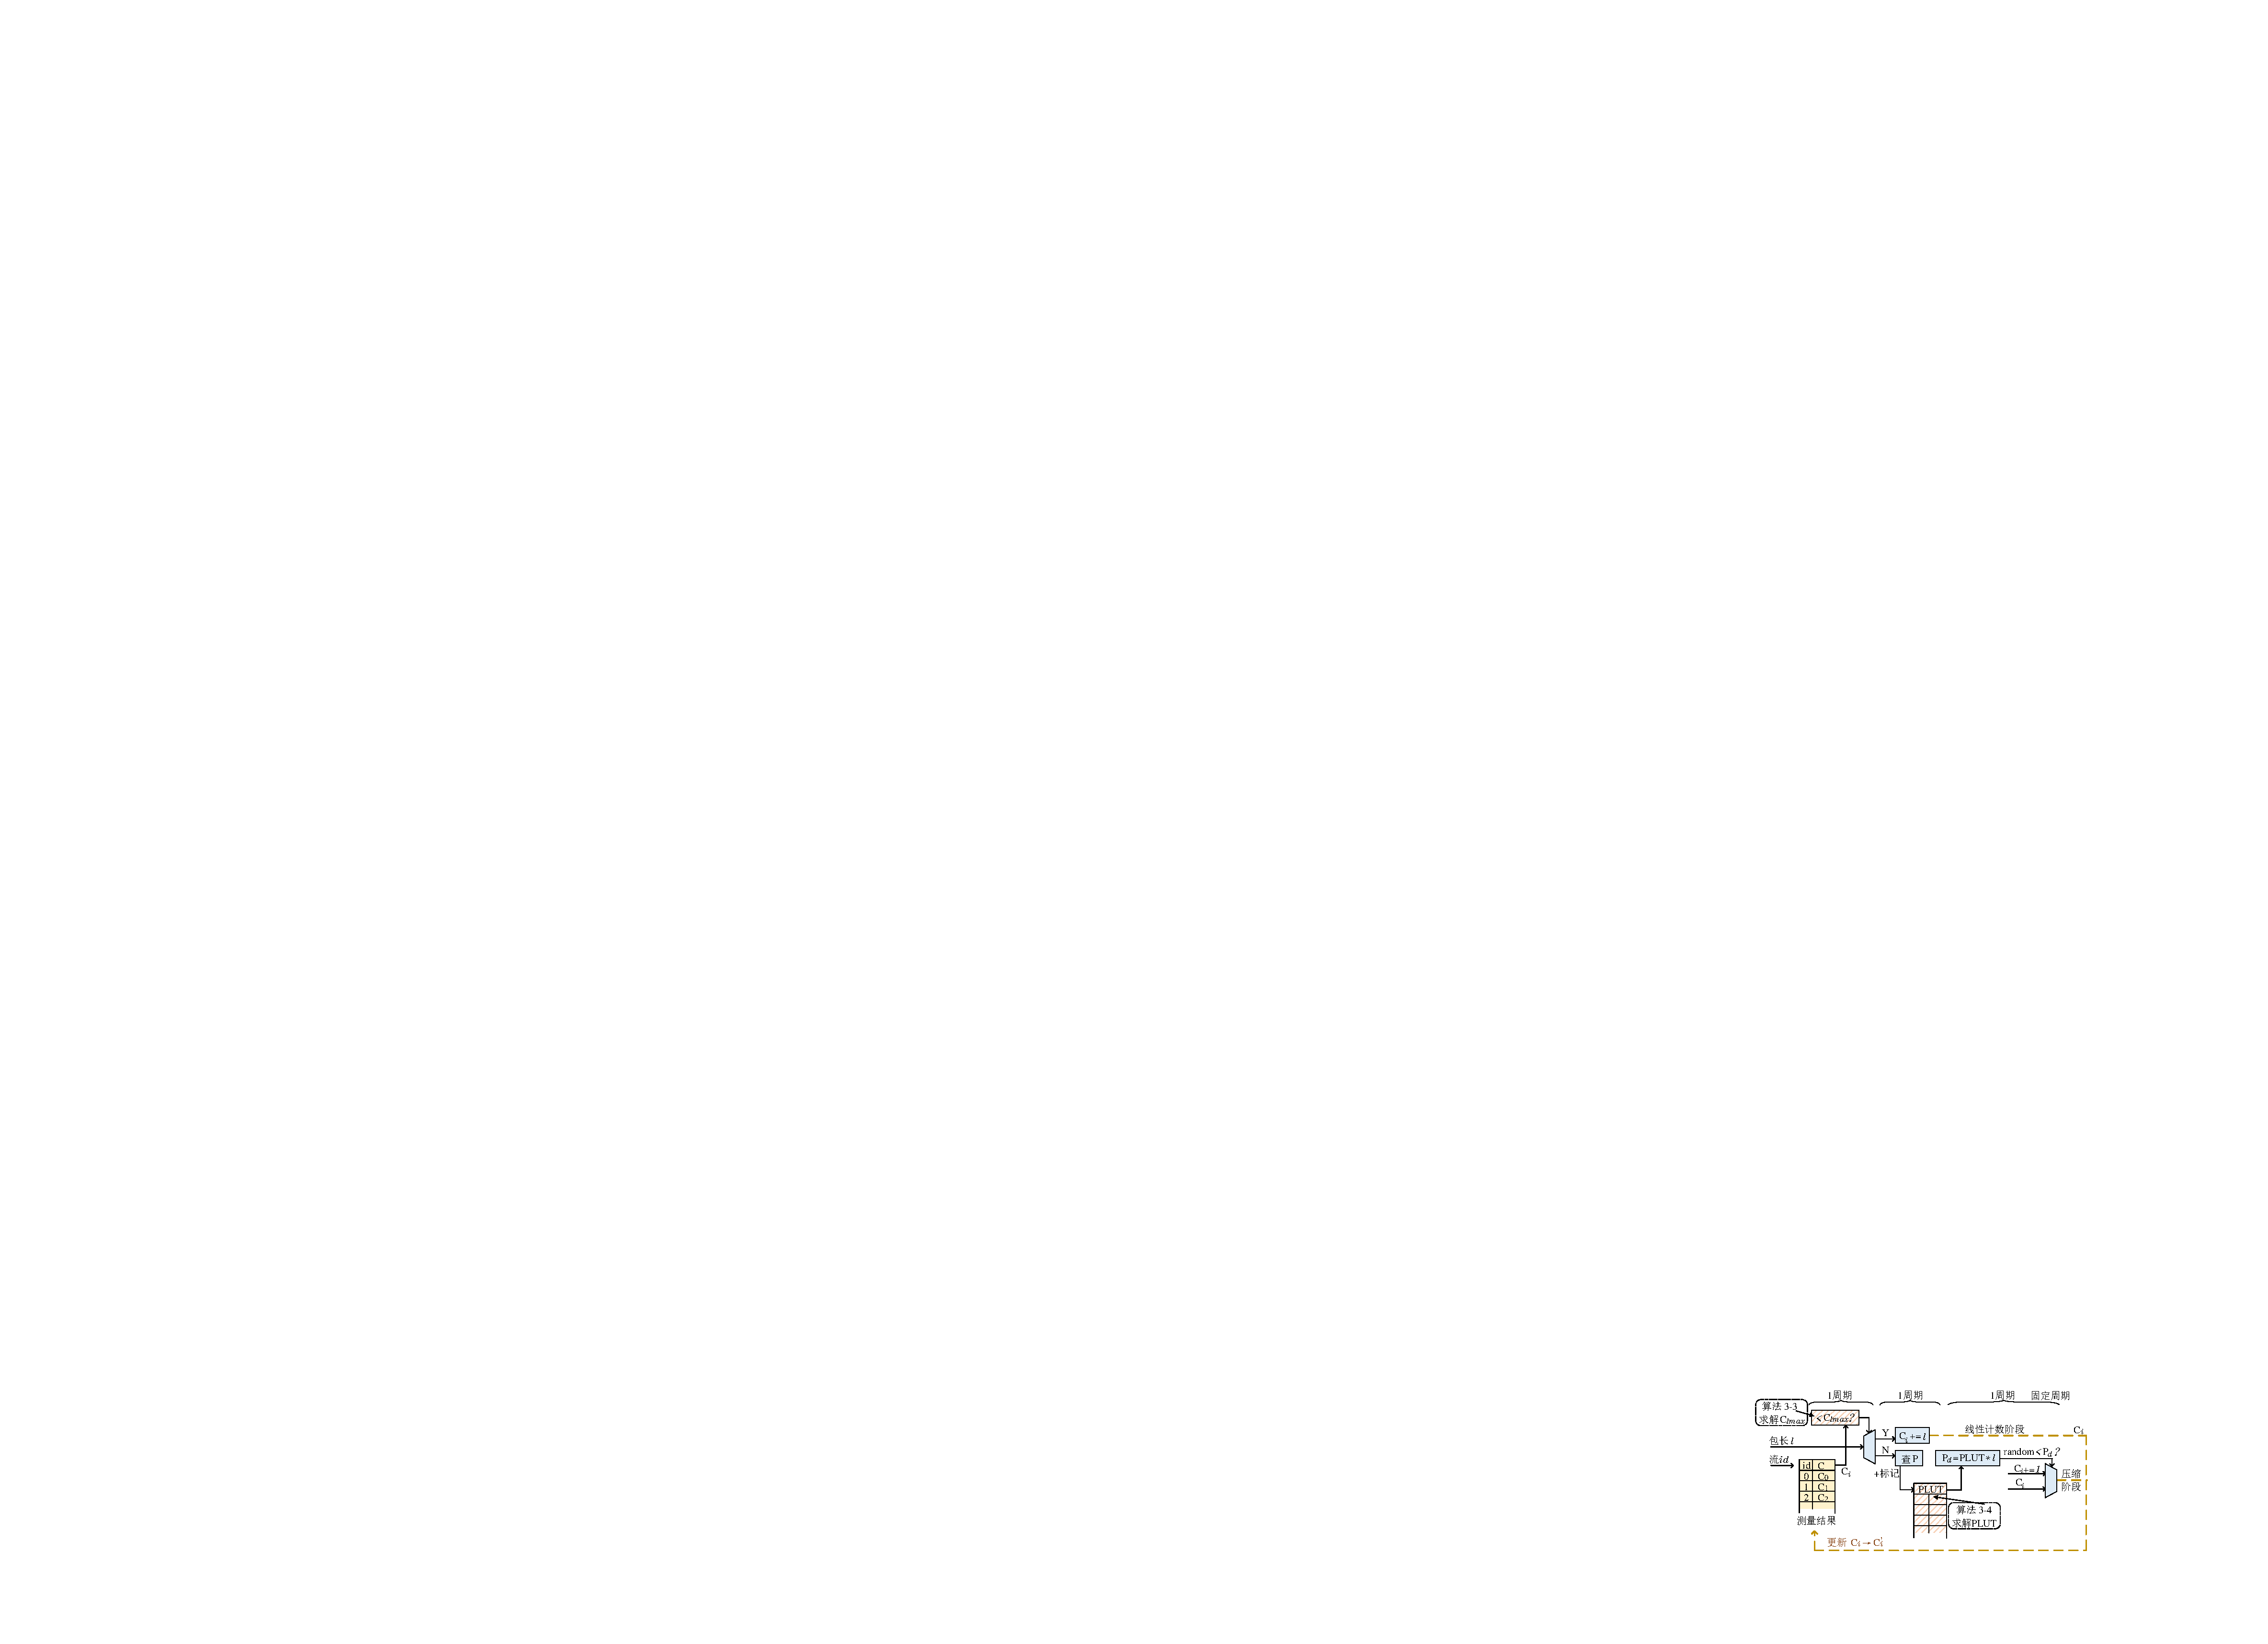
\includegraphics[scale=1]{mydiscopipeline3.pdf}
	\caption{压缩统计硬件流水线设计(优化)} \label{fig:mydiscopipeline}
\end{figure}

图\ref{fig:mydiscopipeline}展示了优化后的压缩计数架构设计(即算法\ref{mydiscoa4}所描述的快速压缩更新的完整过程)。Magic\_Number值由$c_{lmax}$带入函数$f(c)$中得出,第一阶段,系统采用线性增长方式,系统判断当线性增长的统计量大于Magic\_Number后,统计方式改为压缩方法(第二阶段)。为快速区分某统计值所处统计阶段,本文将统计量c的最高位设置为标志记位,当第一阶段时为“0”,第二阶段时须标记为“1”。

\begin{figure}[!ht]
	\centering
	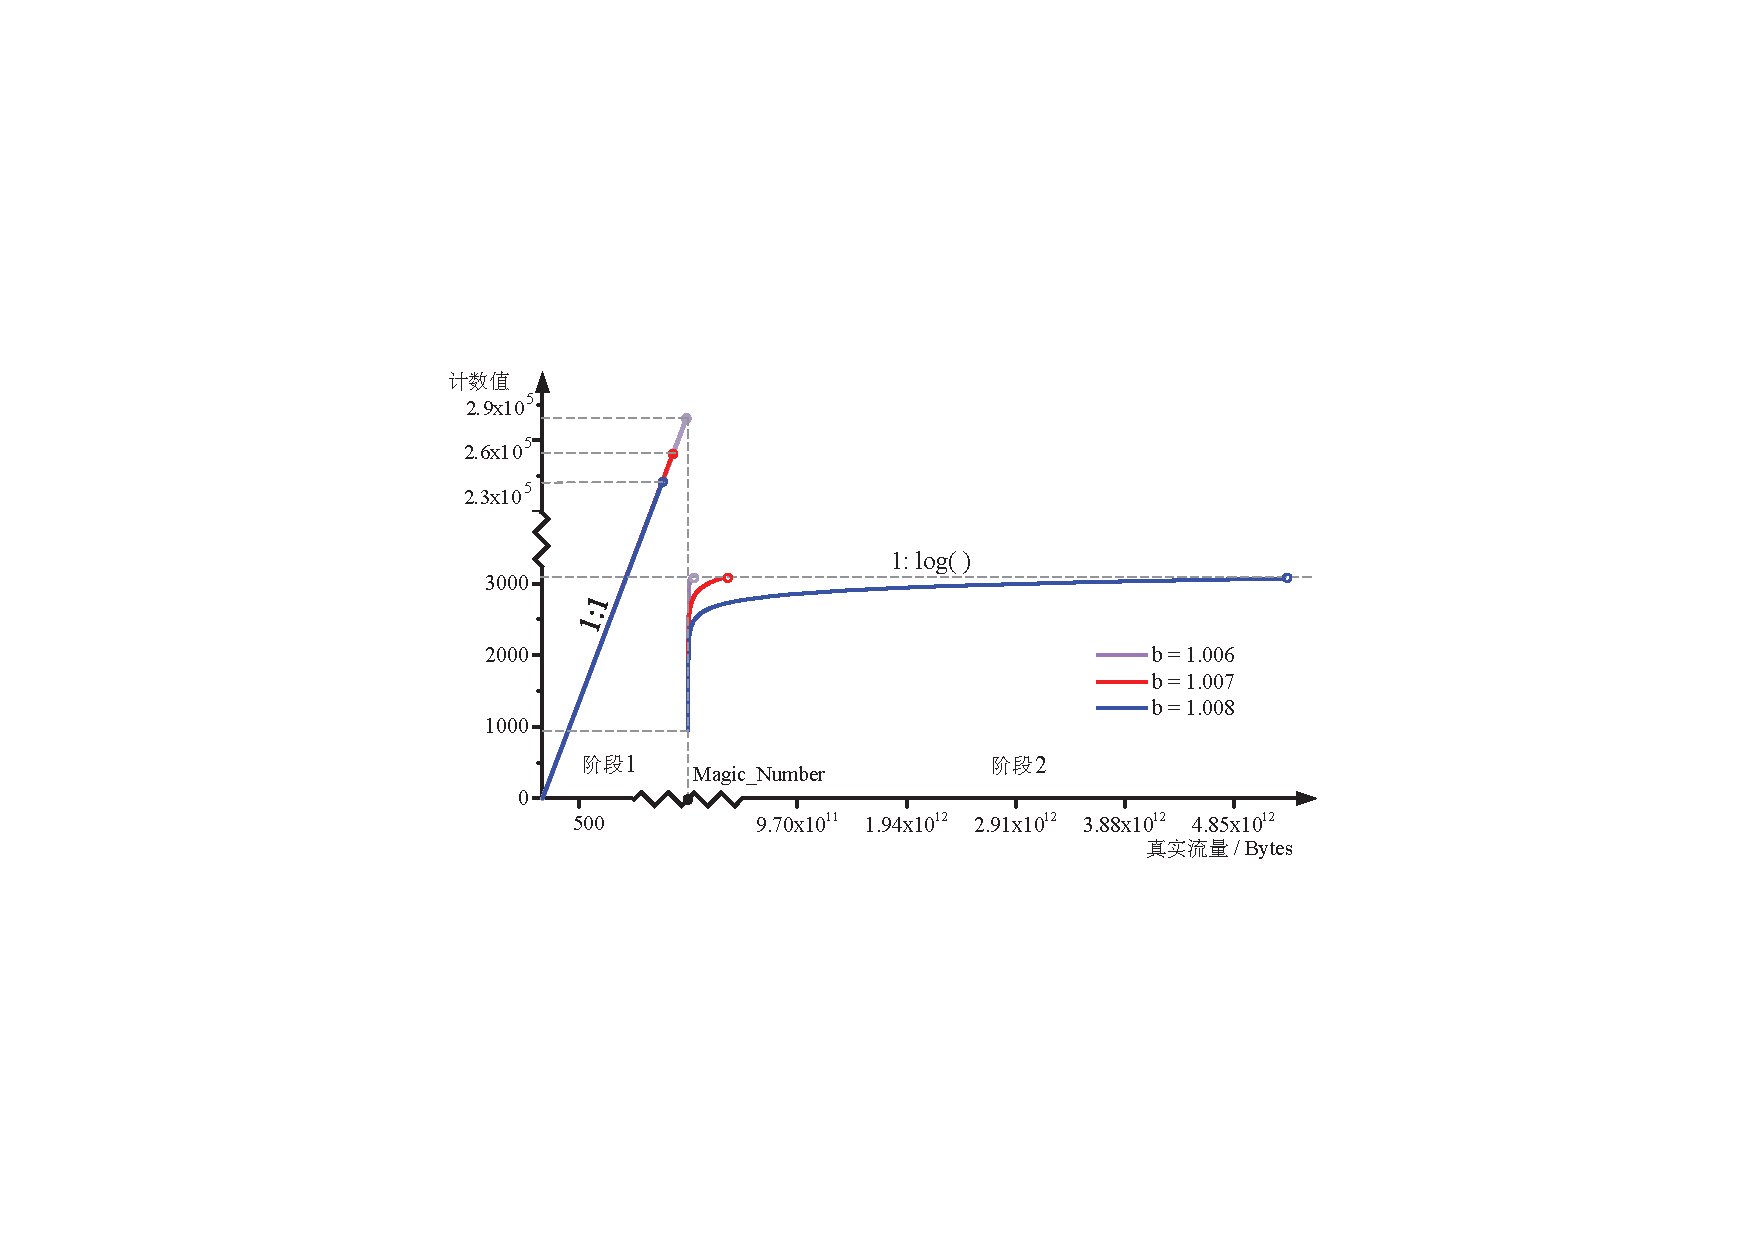
\includegraphics[scale=0.97]{couterqsy1.pdf}
	\caption{不同参数b下的计数曲线} \label{fig:couterqsy1}
\end{figure}

本文提出的新压缩方法具有极大灵活性,在运行时用户可根据自身对于统计精度、统计容量大小(b),资源消耗率(Depth),来自行选择计算查找表内容。如图\ref{fig:couterqsy1},展示了在不同计数容量需求下,修改参数b来扩展计数器统计容量范围(从$1.5\times 10^{10}$Bytes到$5.3\times 10^{12}$Bytes,扩容353倍)。此时计数器位宽(20bits)与查找表PLUT的位宽深度(24bits,3072项)均保持不变。

\begin{figure}[!ht]
	\centering
	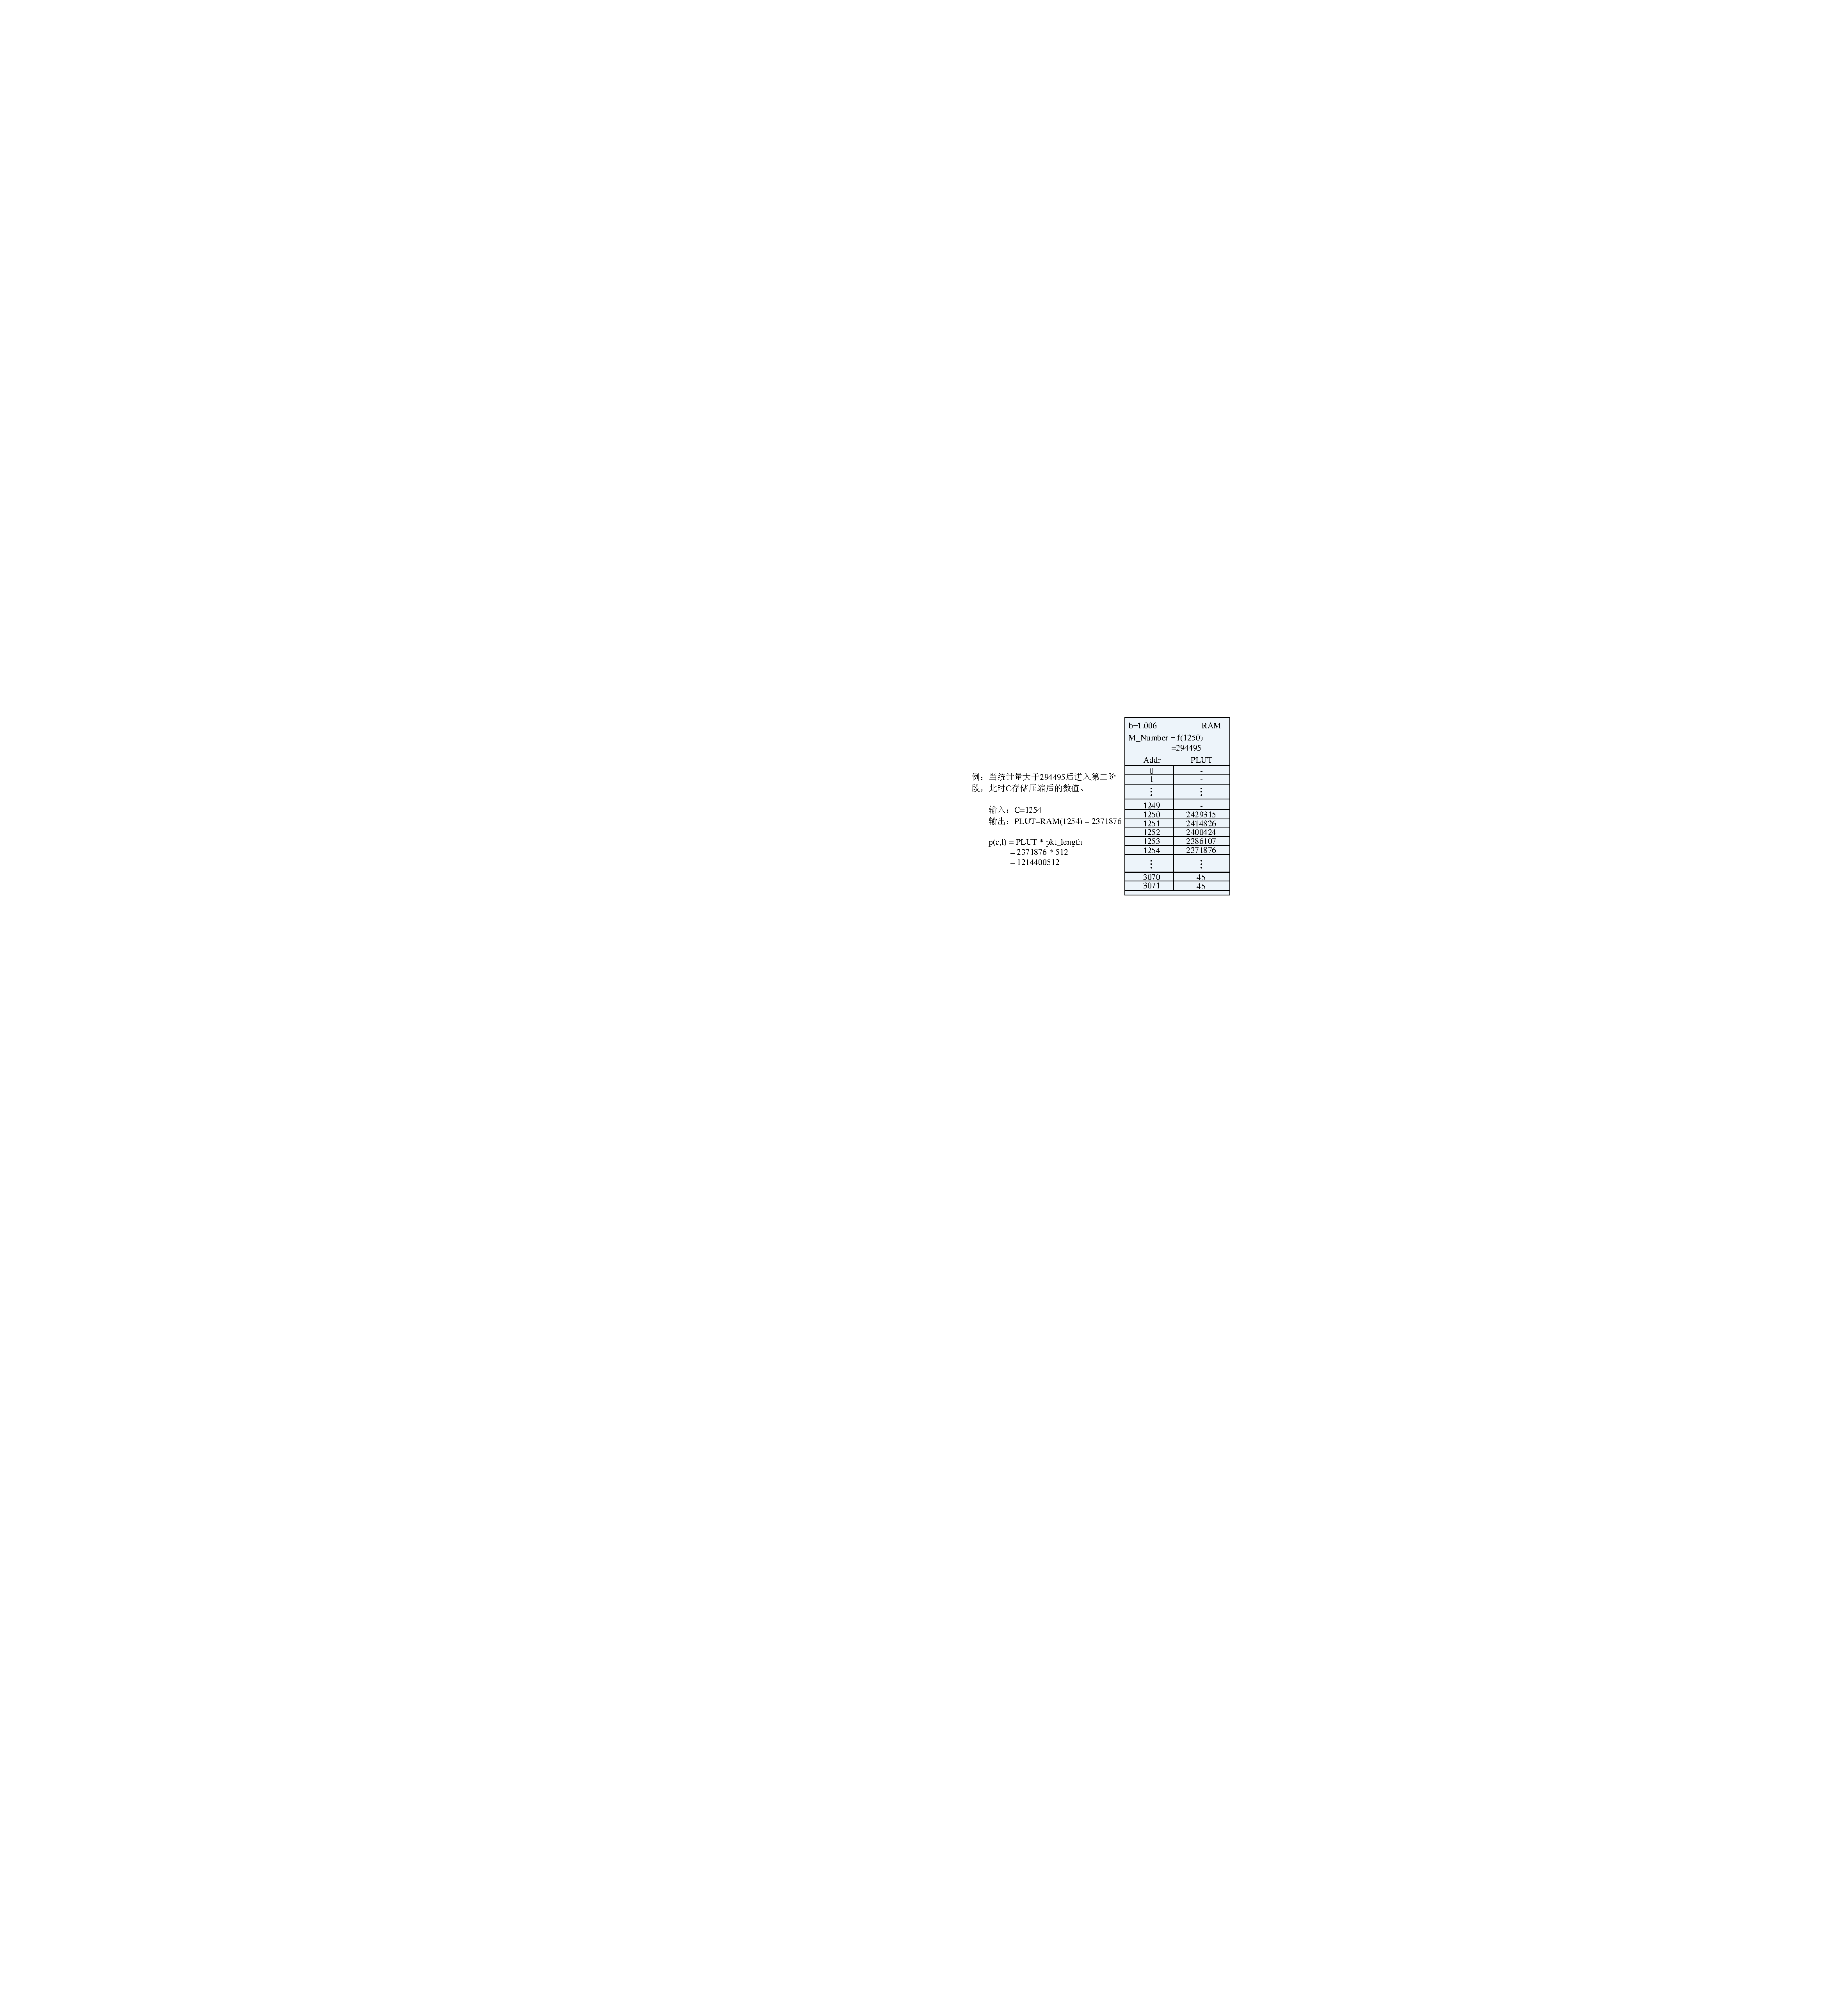
\includegraphics[scale=1]{plut.pdf}
	\caption{b=1.006时的PLUT查找表样例} \label{fig:plut}
\end{figure}

图\ref{fig:plut}展示了当b取1.006,深度3072时,概率查找表(PLUT)存储内容的样例。若线性统计量超过294495后,进入第二阶段进行压缩统计。当此时C存储压缩值为1254,且新入包长为512字节,则经过查表与计算得到$ p_c=RAM(1254)\times pkt\_length= 2371876 \times 512 = 1214400512 $,与随机数生成器比较后判断是否+1,即可获得新的计数值。最终本文将耗时超过50个时钟周期的压缩计算过程缩短到3个时钟周期内完成。

%在实现时,pc的位宽20bits解释一下,总共32bits,然后pc的范围,,,,画总体实现架构,写 表生成的算法,写新算法。给出一个例子。参考论文吧,乔思祎2020年7月12日19:24:45


2)无偏估计证明

整理本文提出的计数器更新规则:

\begin{equation} \label{mydiscof7}
 f(C)=\left\{
\begin{array}{rcl}
C         &      & {C \leq Magic\_Number} \\
\dfrac{b^C-1}{b-1}       &      & {C \geq C_{lmax}}
\end{array} \right. 
\end{equation}

其中$ C $为计数器中存储值,$ b $为固定常数。定义阶段转换时系统状态:


\begin{align}\label{mydiscof9}
f(C_{magic}) &= C_{magic} \nonumber \\
&=\dfrac{b^{C_{lmax}}-1}{b-1} \quad\quad (C_{magic} = Magic\_Number)
\end{align}

本文定义统计过程:统计从第一阶段开始线性累加,当统计量恰好等于$ Magic\_Number $时,转换为第二阶段,其中判断数值$ Magic\_Number $定义。$ C_{lmax} $由(算法\ref{mydiscoa3})由(式\ref{mydiscof9})定义,且此时压缩后的存储值($ C_{lmax} $为压缩后计数的初始值)所表达的实际值由规则$f(C)$(公式\ref{mydiscof7})定义,且初始值所表达真实值与$ Magic\_Number $相等。

本文将证明上述的统计估计函数$f(c)$(c为计数值)在累积统计数据包长度$l$的各个阶段均为无偏估计。首先定义数据包统计过程,不失偏颇,本文假定针对某一条流进行叙述。计数过程的每次累加由数据包触发,假设所有阶段内共有 $ m $ ( $(m\in N^{\ast} $)个数据包到达并触发统计过程。数据包长度分别为$l_1,l_2,\dots,l_m$($ l_i,i\in N^{\ast} $)。$ c_i $为第$ i $个数据包触发系统更新后的计数值。

\begin{theorem}%[Riesz 表示定理]
	$ c $为公式\ref{mydiscof7}中的统计值,其中$ f(c) $为真实统计量的估计值,则$ f(c) $是一种无偏估计。即,对任意$ i\in N^{\ast} $,有:
\begin{equation} \label{mydiscof8}
E[f(c_i)]=\sum ^{m}_{i=1}l_{i}
\end{equation}	
\end{theorem}

\begin{proof}
	首先,考虑函数$ f(c) $的第一阶段。由于线性计数,计数值等于累加值,存在特殊情况$n$($ n\leq m $),使得:

	\begin{equation} \label{mydiscofa}
	c_i=\sum ^{k}_{i=1}l_{i} \quad\quad k \leq n; k,n,m \in N^{\ast}
	\end{equation}
	
	又根据定义(公式\ref{mydiscof7}),可得:
	
	\begin{align}\label{mydiscofb}
	f(c_i) &= c_i \nonumber \\
	&=\sum ^{k}_{i=1}l_{i} \quad\quad k \leq n
	\end{align}
	
	因此:
	
	\begin{align}\label{mydiscofc}
	E[f(c_i)] &= E(c_i) \nonumber \\
	&=c_i \nonumber  \\
	&=\sum ^{k}_{i=1}l_{i} \quad\quad i \leq n
	\end{align}
	
	其次,考虑第二阶段,前文工作\citeup{hu2013discount}已经证明:
	
	\begin{equation} \label{mydiscofd}
	E[\dfrac{b^c-1}{b-1}]=\sum_{i=1}^{m}l_i \quad\quad i \leq m
	\end{equation}
	
	令p为第二阶段内的某一个数据包,即$ n \leq p \leq m $,根据定义\ref{mydiscof9}可得:
	
	\begin{equation} \label{mydiscofe}
		f(c_n) = c_n = \dfrac{b^{c_n}-1}{b-1}\quad\quad p=n
	\end{equation}
	
	由\ref{mydiscofd}与\ref{mydiscofe}得到:
	
	\begin{equation} \label{mydiscoff}
	E[f(c_p)]=E[\dfrac{b^{c_p}-1}{b-1}]=\sum_{i=1}^{p}l_i\quad\quad p=n
	\end{equation}
	
	由于p=n时无偏性成立,因此当p>n时,可直接应用结论\ref{mydiscofd}得证无偏性:
	
	\begin{equation} \label{mydiscofh}
	E[f(c_p)]  = \sum_{i=1}^{p}l_i \quad\quad n<p\leq m
	\end{equation}
	
	联系\ref{mydiscofc}、\ref{mydiscoff}与\ref{mydiscofh}得到:
	
	\begin{equation} \label{mydiscofg}
	E[f(c_p)]==\sum_{i=1}^{p}l_i\quad\quad p \in [1,m]
	\end{equation}
	
	以上证明假定数据包$ 1,2,\cdots,n $恰好组成了第一阶段,且数据包$ n,n+1,p,\cdots,m $恰好组成第二阶段,并得证。另需证明一般情况,Magic\_Number无法由确定数量包长度之和组成,即:
	
	\begin{equation} \label{mydiscofi}
	\sum_{i=1}^{n}l_i < C_{magic} < \sum_{i=1}^{n+1}l_i
	\end{equation}
	
	\begin{figure}[!ht]
		\centering
		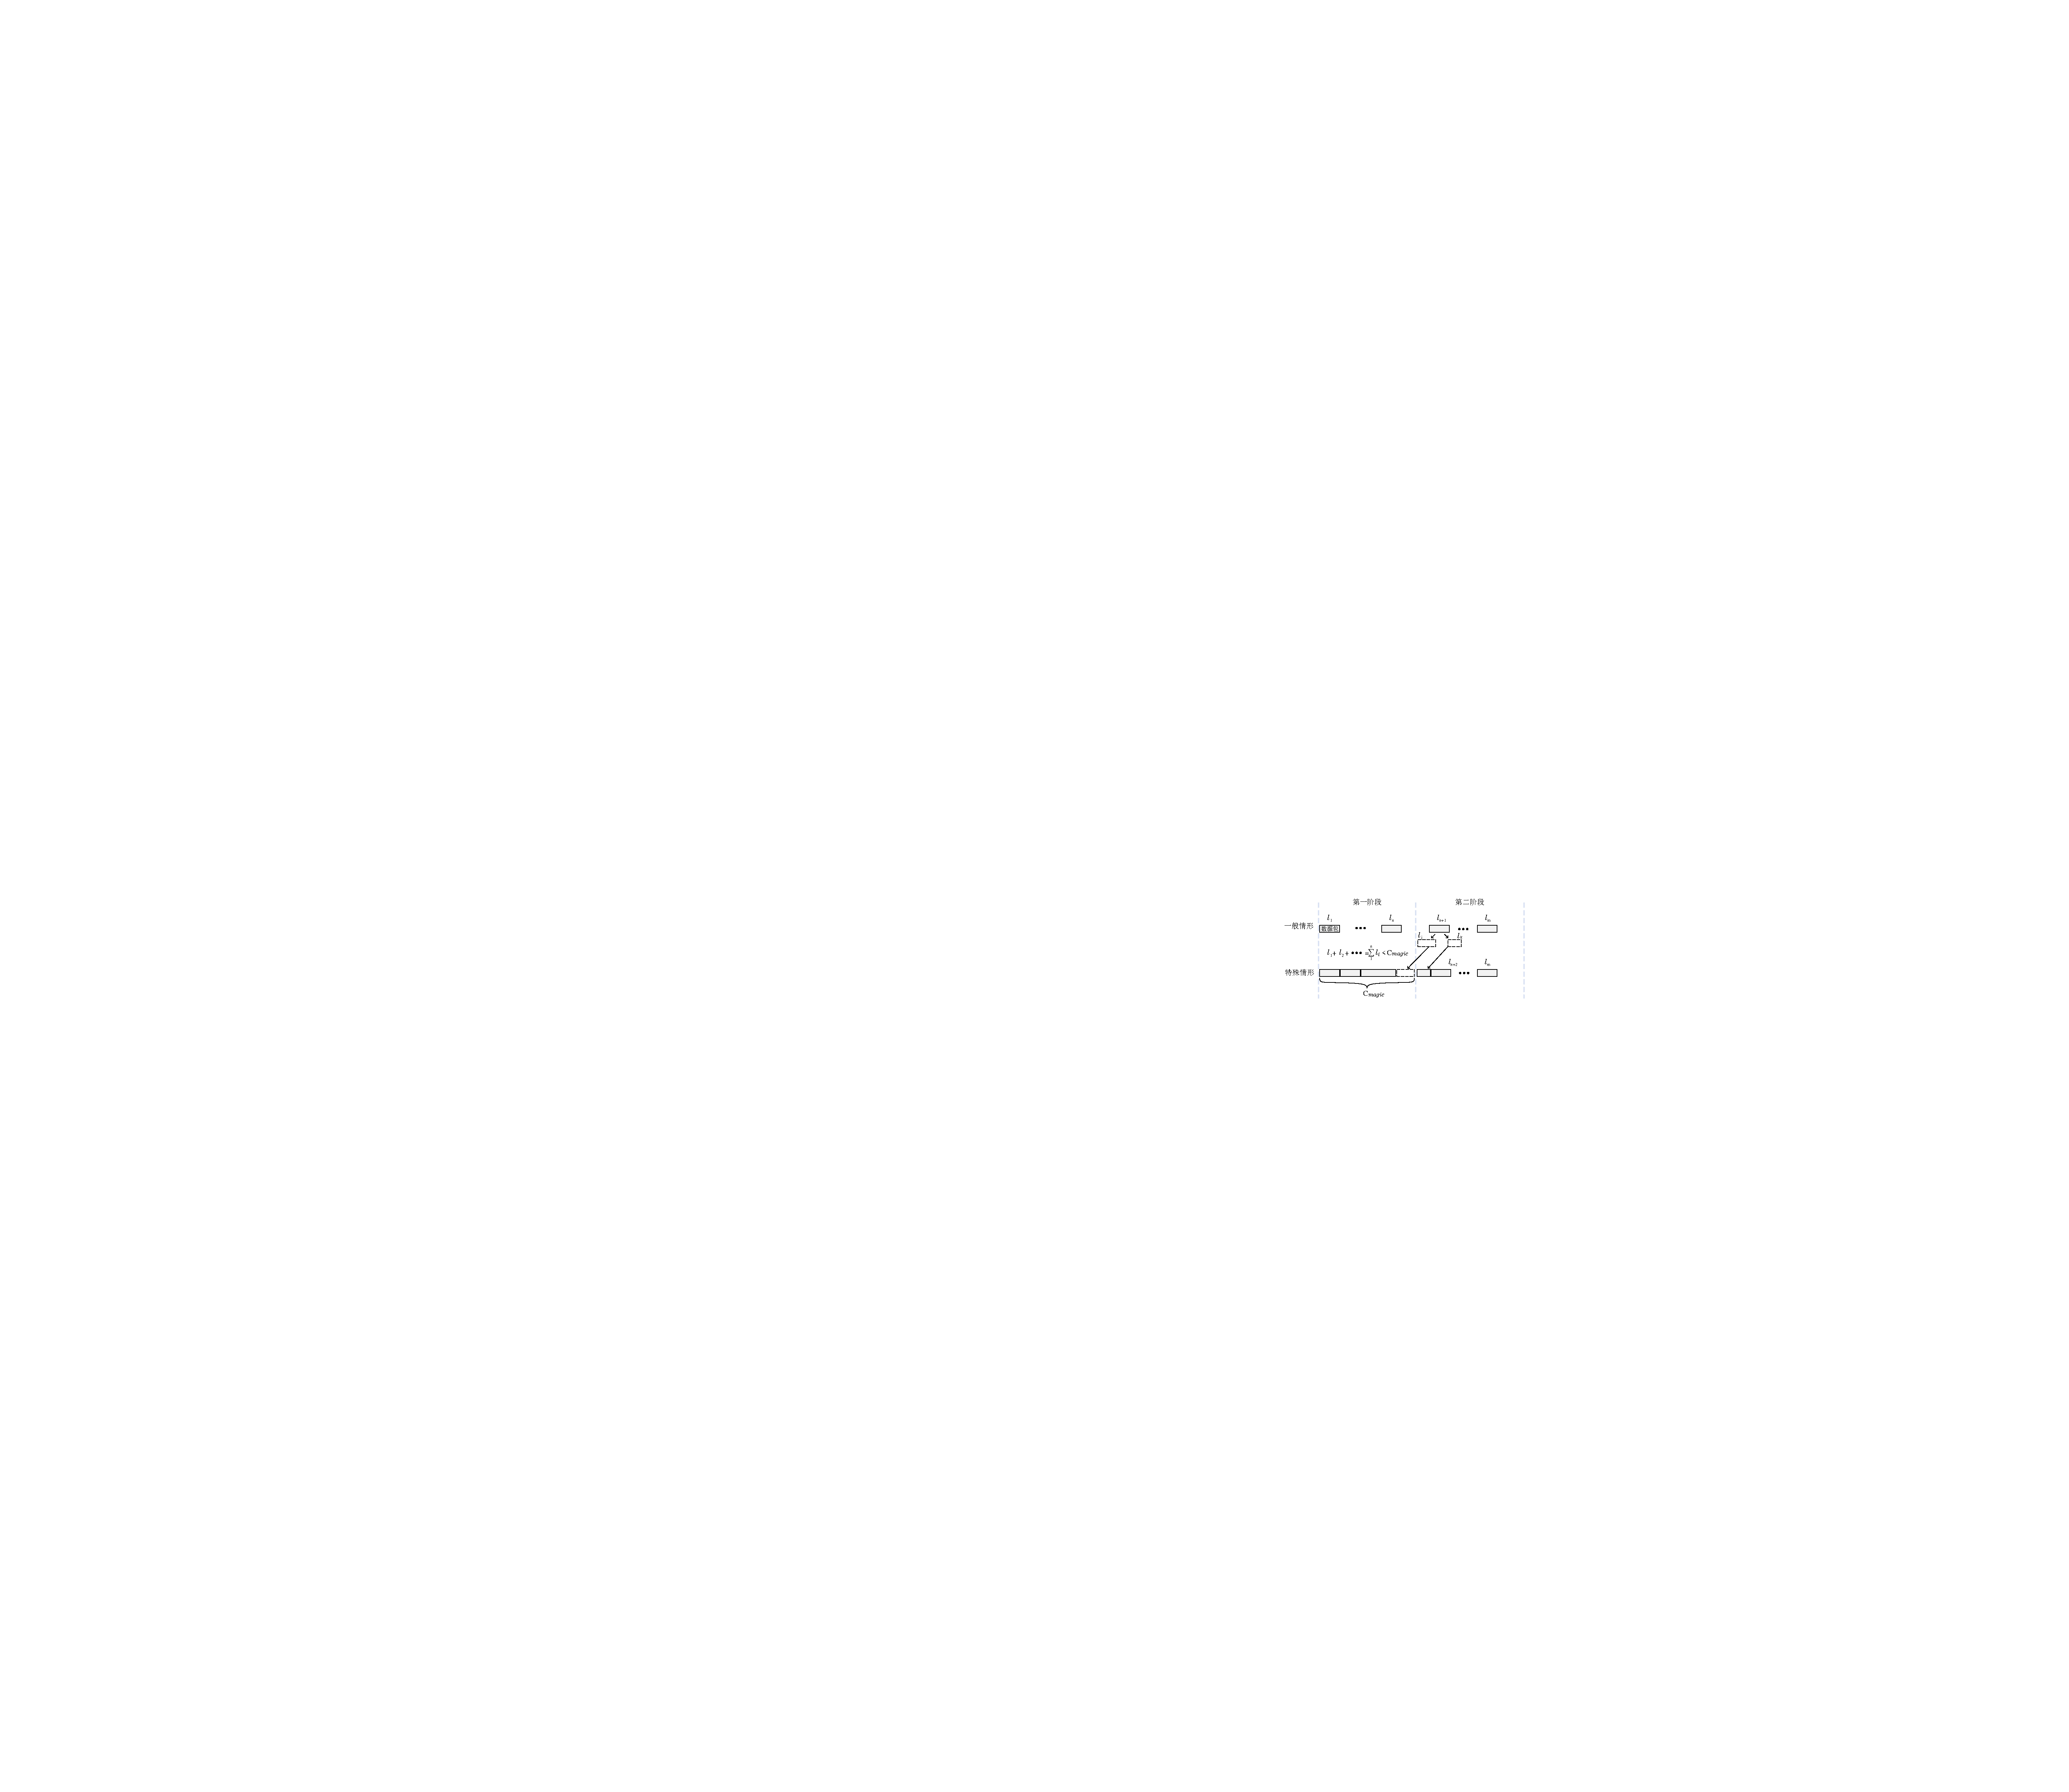
\includegraphics[scale=1]{discozhengming.pdf}
		\caption{一般情形转化为特殊情形得以证明} \label{fig:discozhengming}
	\end{figure}
	
	对此(根据算法\ref{mydiscoa4}),如图\ref{fig:discozhengming},将第$ n+1 $个数据包的包长度$ l_{n+1} $ 分为两部分:$ l_{n+1}=j+k $,得到两个序列$ n'=1,2,\cdots,n,j $,以及$ p'=k,n+1,n+2,\cdots,m $且一定有$ j $使得:
	
	\begin{equation} \label{mydiscofk}
	\left\{
	\begin{array}{rcl}
	E[f(c_{n'})]=\sum_{i=1}^{n'}l_i=\sum_{i=1}^{n}l_i+j=C_{magic}         &      & {n' \leq j} \\
	E[f(c_{p'})] =\sum_{i=1}^{p'} l_i     &      & {j\leq p' \leq m}
	\end{array} \right. 
	\end{equation}
	
	因此,归约到特殊情况的结论(\ref{mydiscofg})。证毕。
\end{proof}

\BiSection{软硬一体化的系统实验平台}{aa} %2

基于软件的网络实现平台,例如OVS,cPqd软件交换机,易于修改与部署,且可以配合网络拓扑仿真框架进行流量测试。但其仿真性能受限于CPU架构,交换性能和仿真时间随着流量和节点的增加而快速变差。这种通常的实验设施无法完成本文对于高精度高性能设计的验证。因此对于本章节介绍的两个关键内容,本文使用基于硬件的真实网卡进行流量测试。本文实现了一款带有PCIe Gen2 $ \times $ 8主机接口的基于FPGA的智能网卡ONetCard。配以相应的软件驱动,实现并打通了数据通路。

\BiSubsection{软件}{aa}

实验平台包括两部分,一部分是主机运行的软件驱动程序,另一部分是FPGA网卡中运行的逻辑编码。数据帧从硬件传输到软件依靠CPU中断的通知,所以当网络中的数据包传输速率非常快的时候,单位时间产生中断次数也非常多,数据包的处理过程被大量中断干扰,从而降低了性能。目前数据从硬件到软件的传输方式通常为DMA,DMA可以减小搬运数据所消耗的CPU时间,从而提升传输效率。针对网络流量捕获和回放的DMA驱动软件模块,通过PCIe接口在主机内存与网卡内收发FIFO直接传递数据。要求高速传输,因此DMA设计的时候要考虑“高带宽,低时延,低中断频率”。本模块大体分为三个主要部分:PCIe,DMA,数据包队列,各个模块功能特性如下:

\begin{itemize}
	\item PCIe模块。PCIe接口为Gen2 $\times$4,总带宽为4$\times$5Gbps=20Gbps。PCIe接口IP采用Xilinx提供的7Series\_IntBlock\_PCIe IP core,总线宽度为128bits,总线时钟频率为125MHz。
	\item DMA模块。使用基于描述符换的Scatter-Gather型DMA。使用多通道DMA,通道数量可配置。低中断频率,在系统内存中设置多块缓存区采用“乒---乓”操作(或基于简单的容量计数以及计时机制)控制中断频率的速度。包计数中断域值(或缓存块大小)计时器均可配置。
	\item 数据包队列。软件中数据包存储队列数可配置。收发队列互相独立,互不干扰。
\end{itemize}

1)从网卡到内存。

主机为每一个收包队列建立一个环形DMA描述符列表,假定包括10个描述符,这10个描述符连续存放。每个描述符信息包括:有效数据包数量,对应缓存起始地址,对应缓存总占用容量。完成之后主机将每个队列的DMA描述符列表首地址写入网卡,并启动队列DMA。网卡DMA被主机启动后,根据主机写入的描述符列表首地址读取每个队列连续两个描述符,仅在首次读取描述符时取两个,其后每次完成一个描述符并更新后再读取下一个。则可以实现网卡上的描述符缓存,保证任意时刻都有描述符待命,以防止读取描述符过程中引起丢包。

2)从内存到硬盘。

使用linux内核的存储外设接口。用户进程通过系统调用write()/read()向磁盘写数据,在内核中文件系统将底层硬盘外设完全抽象化。统一化的调用接口为分层设计:

\begin{itemize}
	\item 虚拟文件系统层(Virtual Filesystem Layer,VFS)。系统调用read()会触发VFS函数,传递文件描述符和偏移量等信息。VFS确定请求的数据是否已在内存缓冲区;若不存在,确定如何继续执行读操作。
	\item 映射层(Mapping Layer)。假设内核必须从块设备上读取数据,这样内核就必须确定数据在物理设备上的位置。这由映射层完成。
	\item 通用块设备层(Generic Block Layer)。内核通过GBL在块设备上执行读操作,启动I/O动作,完成数据传输。
	\item I/O调度层(I/O Scheduler Layer)。在GBL之下是I/O调度层,根据内核的调度策略,对等待的I/O队列排序。
	\item 块设备驱动(Block Device Driver)。BDD通过向磁盘控制器发送响应指令,执行真正的数据传输。
\end{itemize}

本系统实现了流量捕获与回放的吞吐性能为1Gbps,其中捕获步骤中向硬盘写数据是系统最大的瓶颈,这是因为传统大容量机械式硬盘的写入速度慢通常只有400Mbps左右。为日后扩容性能,本文主要分析当前硬盘操作的相关技术发展现状。

在系统写操作(sys\_write())调用结束后,此时要写入的数据其实并没有被立即真正写入磁盘。已写入数据只是被拷贝到内核的缓冲区,并将相应的页标记为脏页。由于系统都需要高速缓存的支持,写操作实际上会被高速缓存延迟进行。当页高速缓存中的数据比后台存储的数据新的时候,该数据被称为脏数据。在内存中累计起来的脏页须最终被写回到磁盘。因而当发生以下两种情况时,写磁盘被触发:

\begin{itemize}
	\item 当空闲内存低于一个特定的域值时,内核必须将脏页写入磁盘,以释放内存空间。
	\item 当脏页在内存中主流时间超过特定域值时,内核必须将超过的脏页写回磁盘,以确保脏页不会无限期驻留内存。
\end{itemize}

进行间隔同步工作的进程名叫pdflush。pdfflush机制存在的问题:在多磁盘系统中,pdflush管理所有磁盘的页/缓冲,从而导致一定程度的I/O瓶颈。从内核2.6.32开始,终止了pdflush机制,改成了bdi\_writeback机制。新机制为每个磁盘都创建了一个专门线程,负责这个磁盘的页缓存数据刷新,从而实现了每个磁盘数据刷新程序在线程级别的分离,以提高I/O性能。另外目前固态硬盘(SSD)硬盘技术发展迅速,单块固态硬盘写入速度可高达10Gbps,因此为日后系统升级铺平了道路。

\BiSubsection{硬件}{aa}

为实现高精度的流量时间标注以及回放功能,本文实现了一款带有PCIe Gen2 $ \times $ 8主机接口的基于FPGA的智能网卡ONetCard(图\ref{fig:onetcard}示)。

\begin{figure}[!ht]
	\centering
	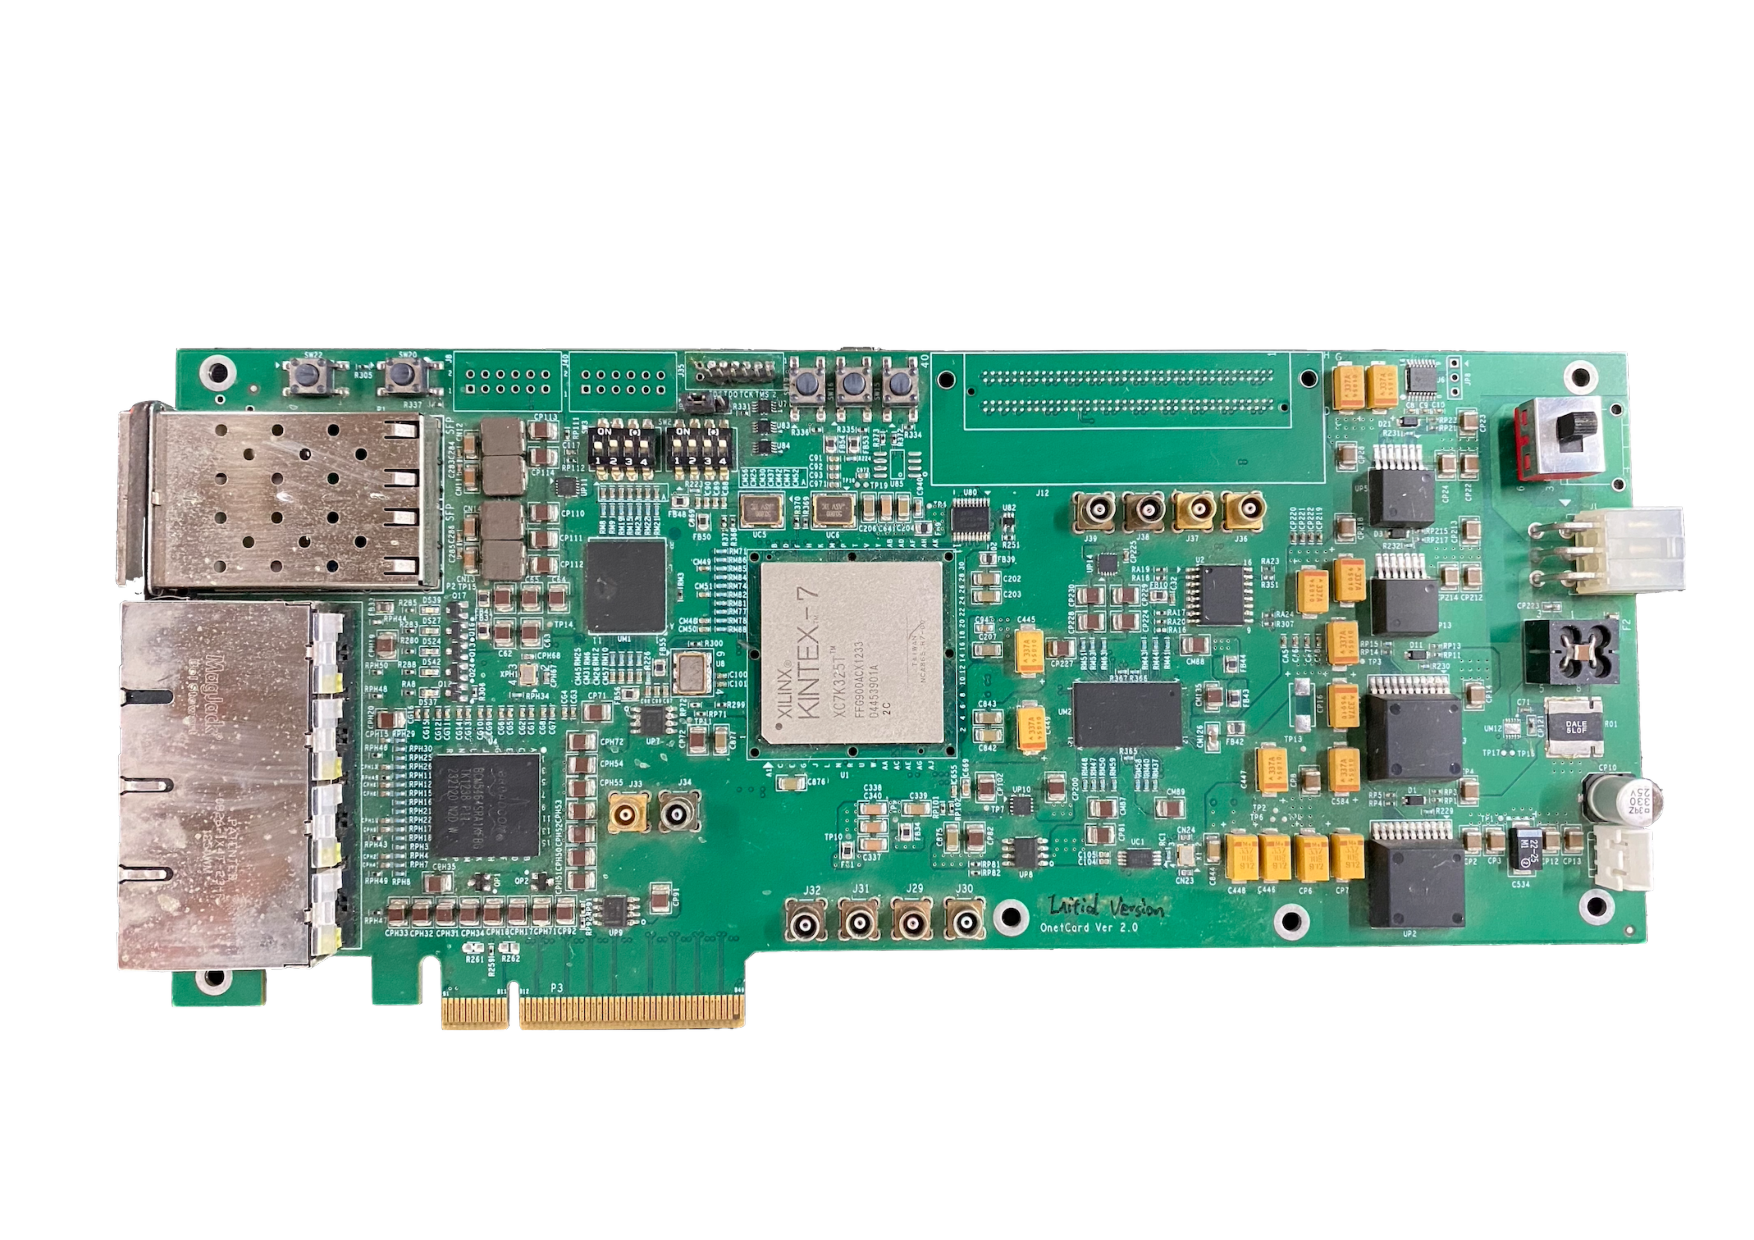
\includegraphics[scale=0.46]{onetcard.pdf}
	\caption{用于测试基于FPGA网卡的流量捕获功能的ONetCard实验平台} \label{fig:onetcard}
\end{figure}

该网卡的核心器件使用Xilinx公司FPGA产品XC7K325T,约有33w个可编程逻辑单元。为支持高速随机缓存和查找功能,FPGA外部搭配了一块9MB的QDR SRAM,以及72MB的RLDRAM。网络接口部分有四个G比特电口和两路SFP+万兆光口。PCIe提供Gen2$\times$8标准,总带宽达40Gbps。板卡预留有FMC接口,可外扩高速串行总线的设备或接口,例如TCAM查找表、存储器、网络接口等。板卡尺寸与NetFPGA类似,但是能够提供的可编程逻辑数目更多,存储器种类更丰富。本文中的实验板卡可为各类网络计算加速应用提供工程实践支持。

\BiSection{系统评价}{aa}

\BiSubsection{网络流量捕获与回放系统评估}{aa}

基于ISD14.1及其自带仿真工具isim,本文对数据通路中各个子模块分别进行功能仿真验证,最后通过上板测试符合时序约束的逻辑,系统运行在125MHz频率下。

1)增加时间戳。

该模块为进入数据通路的数据包添加时间戳信息,输入数据和输出数据的四组信号如图\ref{fig:addtimestamp}所示,该模块在一级包头后面添加了控制字FE与对应的时间计数器数值。

\begin{figure}[!ht]
	\centering 
	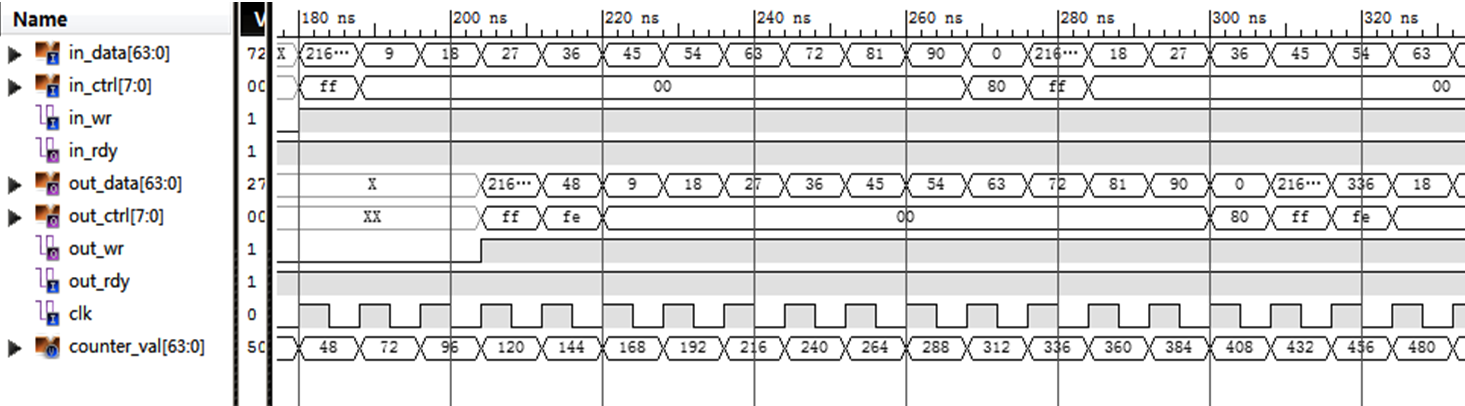
\includegraphics[width=0.95\textwidth]{addtimestamp.png}
	\caption{包头添加时间戳仿真结果} \label{fig:addtimestamp}
\end{figure}

\begin{figure}[!ht]
	\centering 
	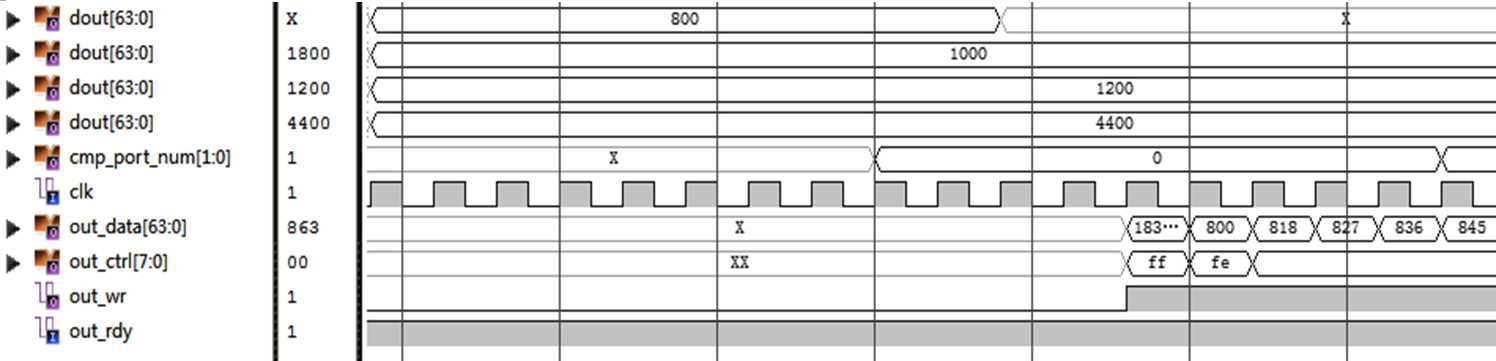
\includegraphics[width=0.95\textwidth]{timecmp.png}
	\caption{时间戳比较器测试仿真结果} \label{fig:timecmp}
\end{figure}

2)回放数据包时间戳比较

验证时间戳排序比较器的功能,如图\ref{fig:timecmp}最上方是四个时间戳FIFO的数值。分别是800、1000、1200、4400对应1、2、3、4路DMA写入网卡的队列。第一路时间戳为800是时间最小的,应该最早被输出。cmp\_port\_num代表比较后的输出队列序号,可以看到有效的第一个值是0。这个数据将送给调度模块,控制其向后传送数据的通道来源,最终由out\_data等信号输出端口输出按时间顺序排列的数据包。

在样机测试中,实验使用发包仪向板卡1Gbps接口中发送了127,503,023个64字节最小数据包。流量分流机制均匀地向四个队列分流了全体数据包,四个队列共计接受数据包个数分别为,31875756,31875755,31875756,31875756。在回放测试中我们从四块硬盘中分别向网卡发送了44160639,44160639,44340794,44316028个数据包,共计176978100个数据包。数据包均按照正确的顺序向外发送,并且无丢包现象。

\begin{figure}[!ht]
	\centering 
	
\includegraphics[scale=1]{expcaprep.pdf}
	\caption{回放时间精度实验拓扑} \label{fig:expcaprep}
\end{figure}

3)回放数据包精度

为测试数据包的回放真实精度,本实验设置了两台主机,如图\ref{fig:expcaprep}所示,每台主机内配置一个智能网卡。

\begin{itemize}
	\item 主机1,捕获数据包,并为数据包增加入队时间戳(timestamp1),以记录数据包真实到达时间分布。之后,对捕获的数据包进行回放。
	\item 主机2,接受主机1发送的回放数据包,并第二次为其增加时间戳(timestamp2)包头。将所有的数据包捕获并存储。
\end{itemize}

\begin{figure}[!ht]
	\centering 
	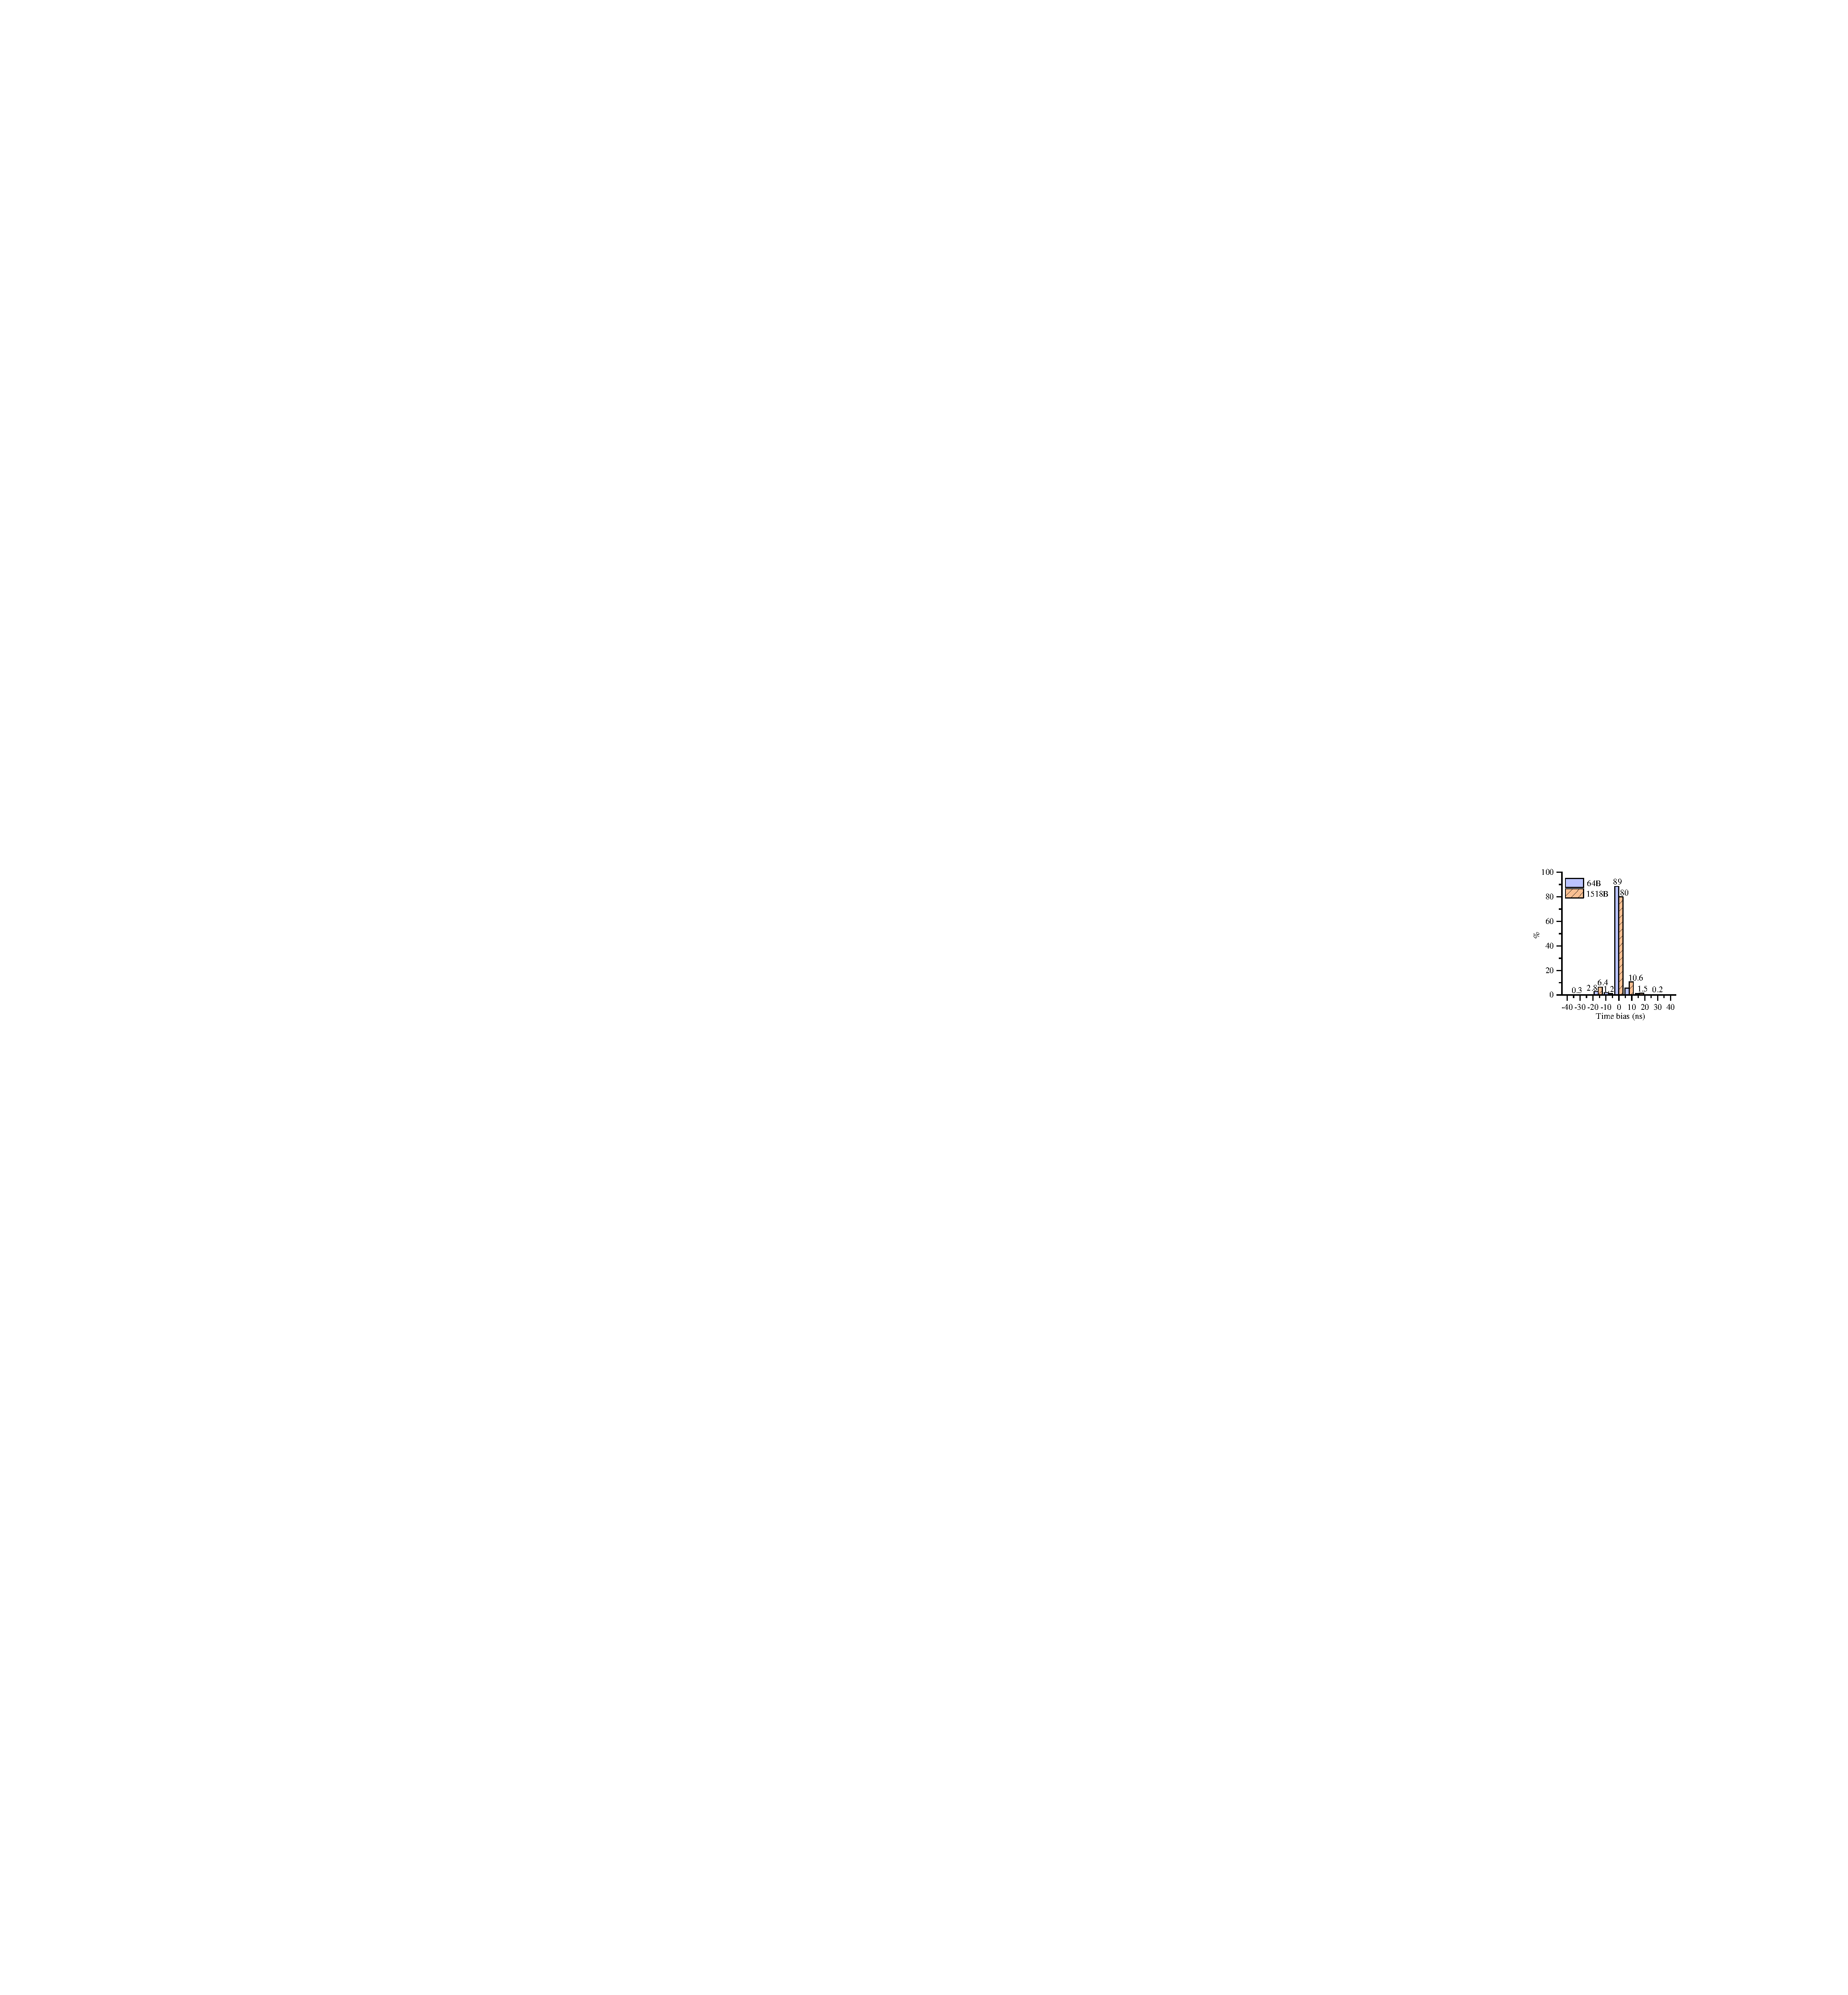
\includegraphics[scale=1]{timebias.pdf}
	\caption{数据包回放时间精度概率分布} \label{fig:timebias}
\end{figure}

因此本文可根据每个数据包包头时间戳来得到其真实到达时间分布,以及经过本系统捕获和回放之后的输出时间分布。

如果系统不会引入时间误差则每对相邻数据包之间的时间间隔均相等。定义捕获数据包的时间间隔$ \Delta timestamp1_n = timestamp1_{n+1} - timestamp1_{n} $,回放数据包的时间间隔$ \Delta timestamp2_n = timestamp2_{n+1} - timestamp2_{n} $,时间系统误差$ (time\_bias_n)=\Delta timestamp2_n - \Delta timestamp1_n $。



实验中本文分别测试了最大包(1518字节)与最小包(64字节),在1Gbps吞吐下的时间误差time\_bias。如图\ref{fig:timebias}所示,回放数据包中有将近80\%可满足无时间误差。系统最大误差只有32ns,即4个时钟周期时间长度。

%画图,,实验拓扑,两个结果图。。。

\BiSubsection{网络测量实时压缩系统评估}{aa}

本实验\footnote{本实验为作者在赛灵思亚太研究院访问实习期间完成。本研究西安交通大学与赛灵思亚太研究院为共同第一完成单位。}目标为100G在线实时进行压缩测量,使用新一代的Xilinx FPGA智能网卡Alveo U250。板卡有2个100G光纤网口,配有PCIe Gen3$ \times $16,与主机互通接口带宽可达128Gbps。

1)测量性能。

本文将测量基于FPGA智能网卡的压缩统计速度,并与DISCO算法,以及Cacti系统相对比。 如图\ref{fig:discothroughput}本文对比了基于x86平台的DISCO算法,DISCO运行时占用一个处理器核心的计算能力。另外本文还对比了相似工作CACTI,CACTI对DISCO在某种情形下做了优化。CACTI利用少量(16个)硬件高速计数器在数据平面内对流量做线性统计,之后定期将少量统计结果上报控制器,在控制器内对统计数量进行DISCO算法压缩。由于减小了压缩频率,因此CACTI能够获得比DISCO更高的吞吐性能。

\begin{figure}[!ht]
	\centering 
	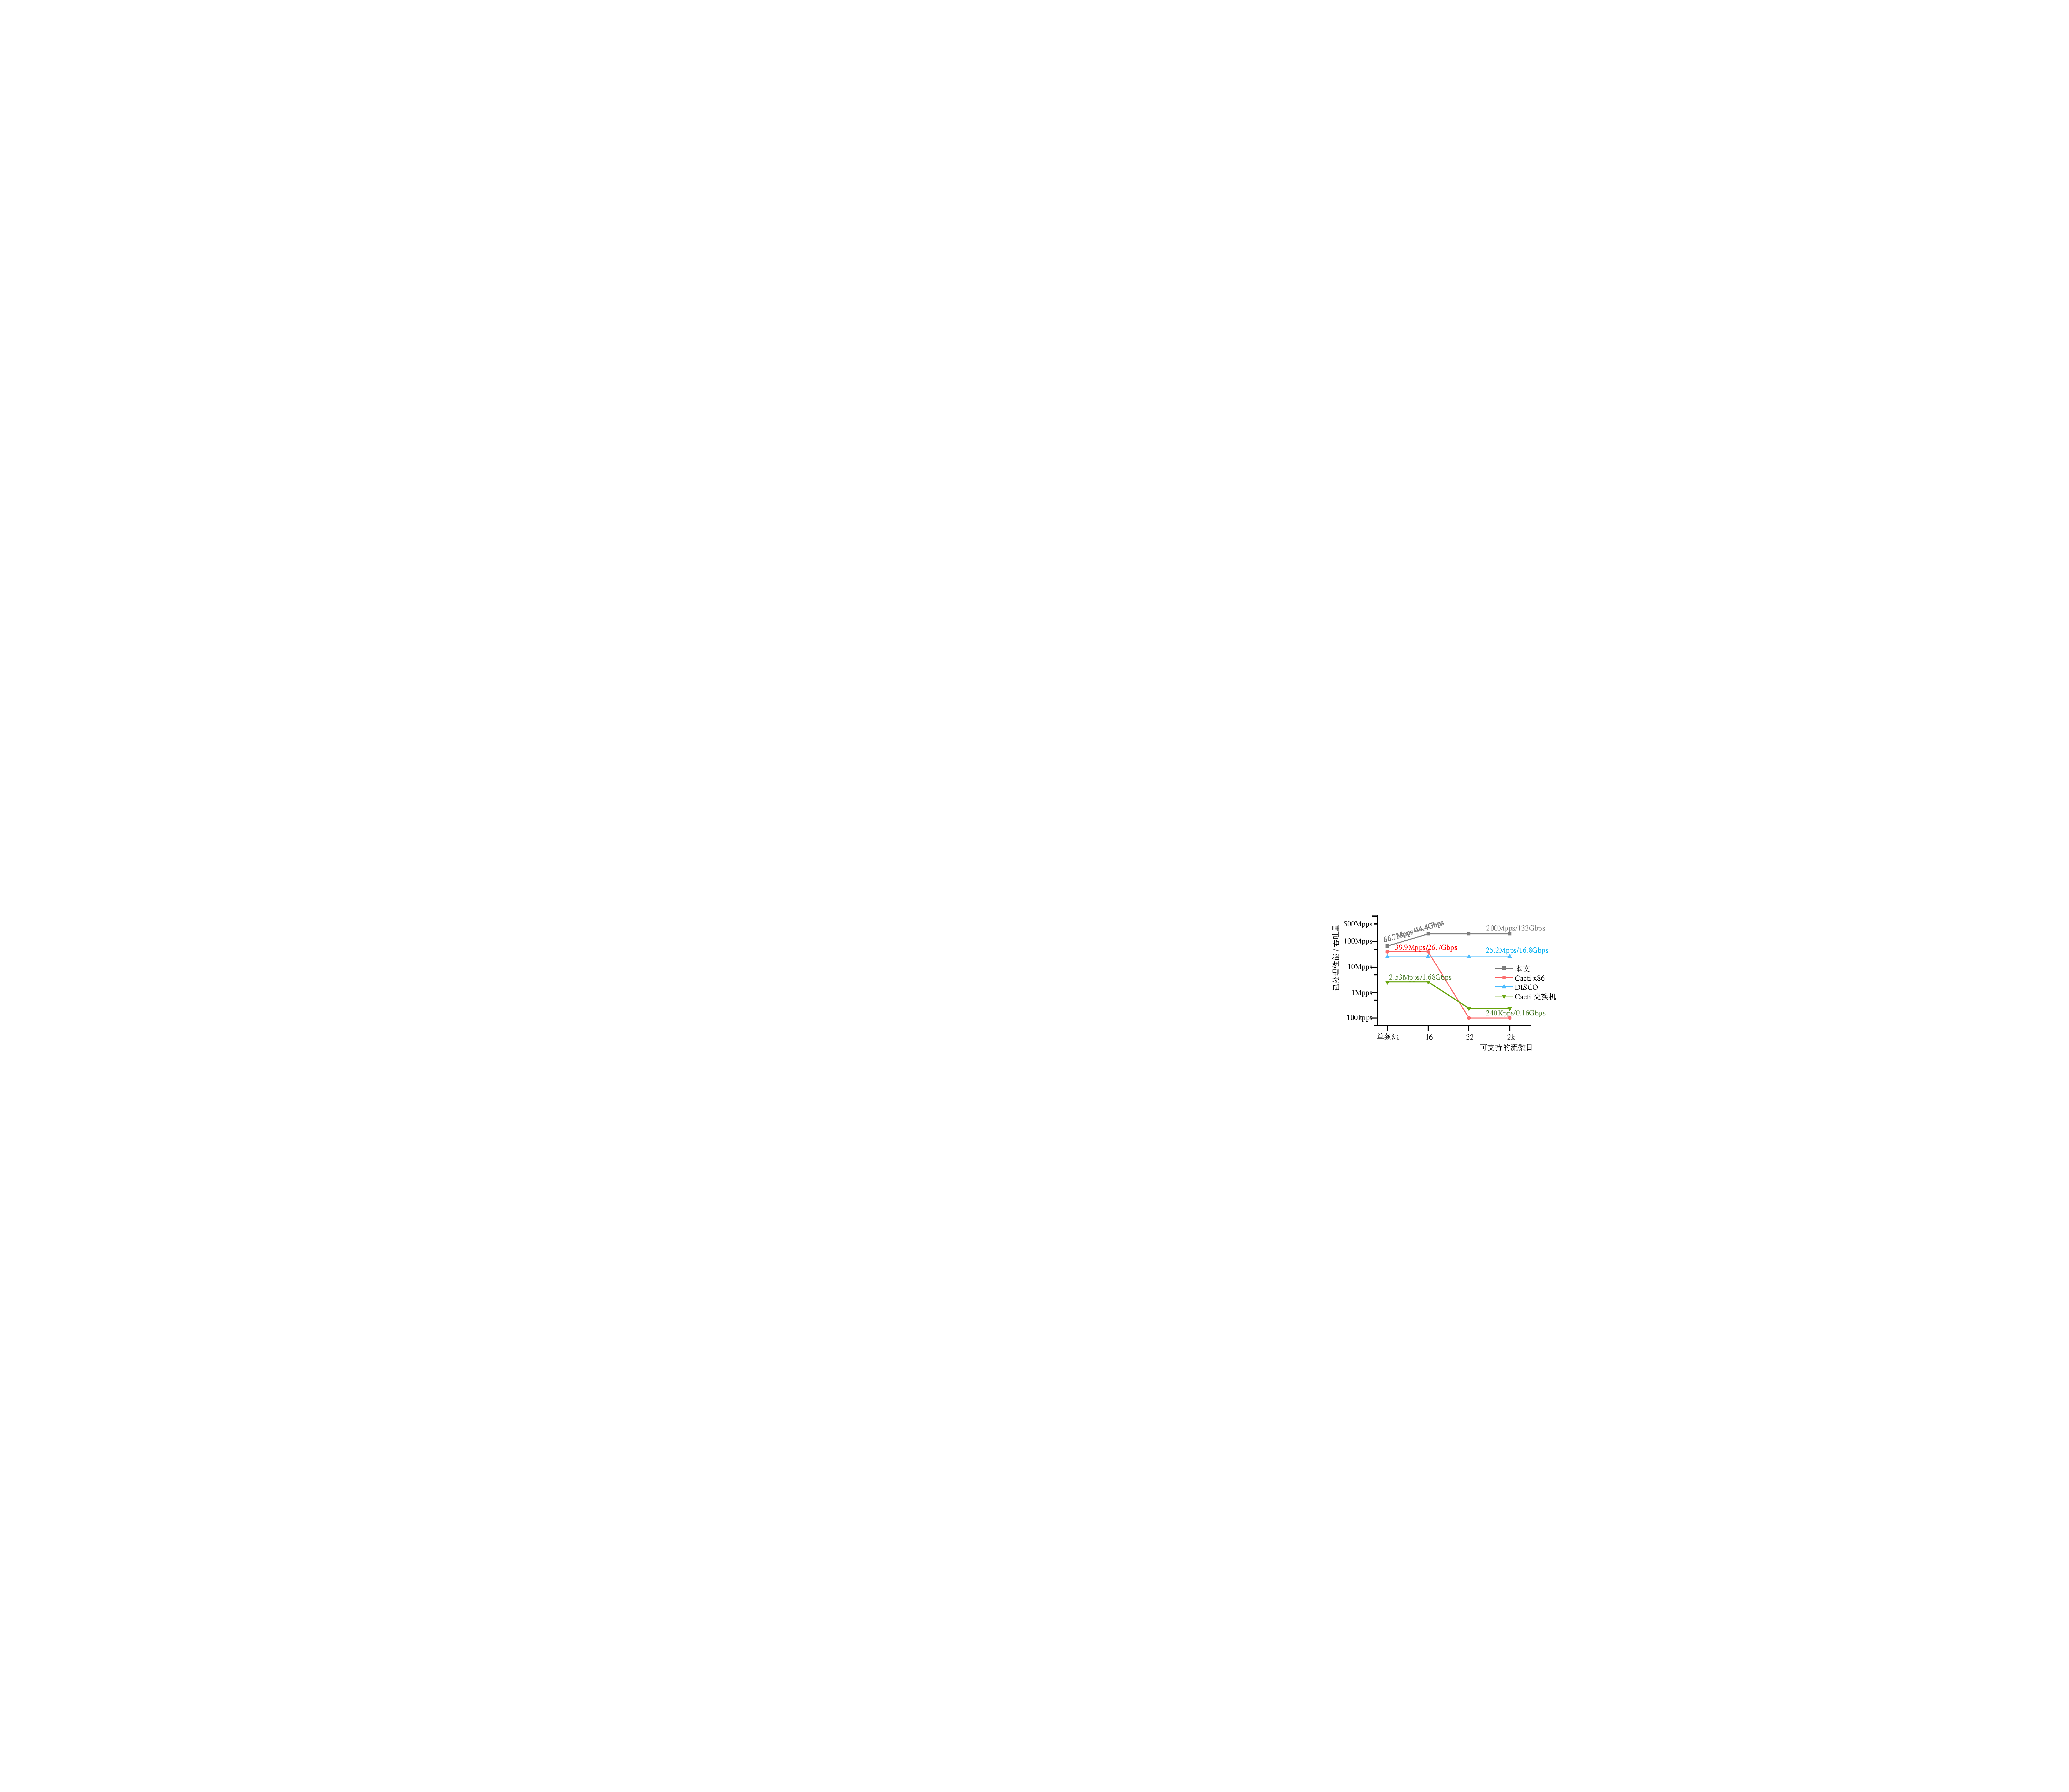
\includegraphics[scale=1]{discothroughput.pdf}
	\caption{本文基于FPGA智能网卡压缩算法与其他压缩统计方法性能对比(64字节小包)} \label{fig:discothroughput}
\end{figure}

对于CACTI系统,当流数目增多,硬件计数器需要频繁向CPU发送缓存更新请求。由于硬件计数器与CPU通信依然依赖于PCIe带宽(此类通信属突发传输),且系统不可占用过多通信管道资源,因此其系统设计时的最高通信容量只有100kpps\citeup{yangjidoc}。一旦流数目超过了硬件计数器数量则系统会频繁请求更新,因此成为系统瓶颈理论性能大幅降低。本文实现的压缩统计最高需要耗费3个时钟周期,且对于同一条流的测量更新是阻塞的(更新时无法继续处理同一条流的后续请求),因此在测试单条流的测量时,性能只有理论最优的三分之一。当流数目多于三种时,每个更新请求可以按流水线方式进入处理通路,因而可以做的每包的单周期吞吐,64字节小包处理性能可达到133Gbps。


\begin{figure}[!ht]
	\centering 
	
\includegraphics[scale=1]{discocpu.pdf}
	\caption{基于FPGA网卡硬件流量压缩统计系统可有效降低主机CPU消耗(64字节小包)} \label{fig:discocpu}
\end{figure}


2)主机CPU资源消耗。

DISCO与CACTI的压缩过程均由CPU完成,当压缩任务请求频次增加,CPU计算资源相应增加。如图\ref{fig:discocpu}所示,实验为处理64字节小包时的最高性能情形下所对应的CPU占用率。本文将所有密集型计算任务均下方到基于FPGA的智能网卡,主机CPU只按需定期查看计数器值即可,无需做额外复杂任务,从而将服务器CPU资源最大限度释放。



3)存储资源消耗。

通过不同方法实现1百万条流的统计所需求的存储空间如图\ref{fig:discomem},对一条流进行简单线性叠加计数只需要开辟流对应的存储空间即可,在未优化的情形下一般需要为每一条流开辟32bits计数空间,然而此空间有固定上限(4GB)一旦超出需要开辟更大空间,或提前上报。可压缩的计数方式上限较高,本文在压缩率达到38\%时,计数上限可达100GB,比固定上限值大25倍。可压缩计数方式可以灵活且低成本地扩展计数上限。DISCO、CACTI等压缩算法不同设计方式会额外占用不同大小的固定空间(计算表),但总体差别不显著。

\begin{figure}[!ht]
	\centering 
	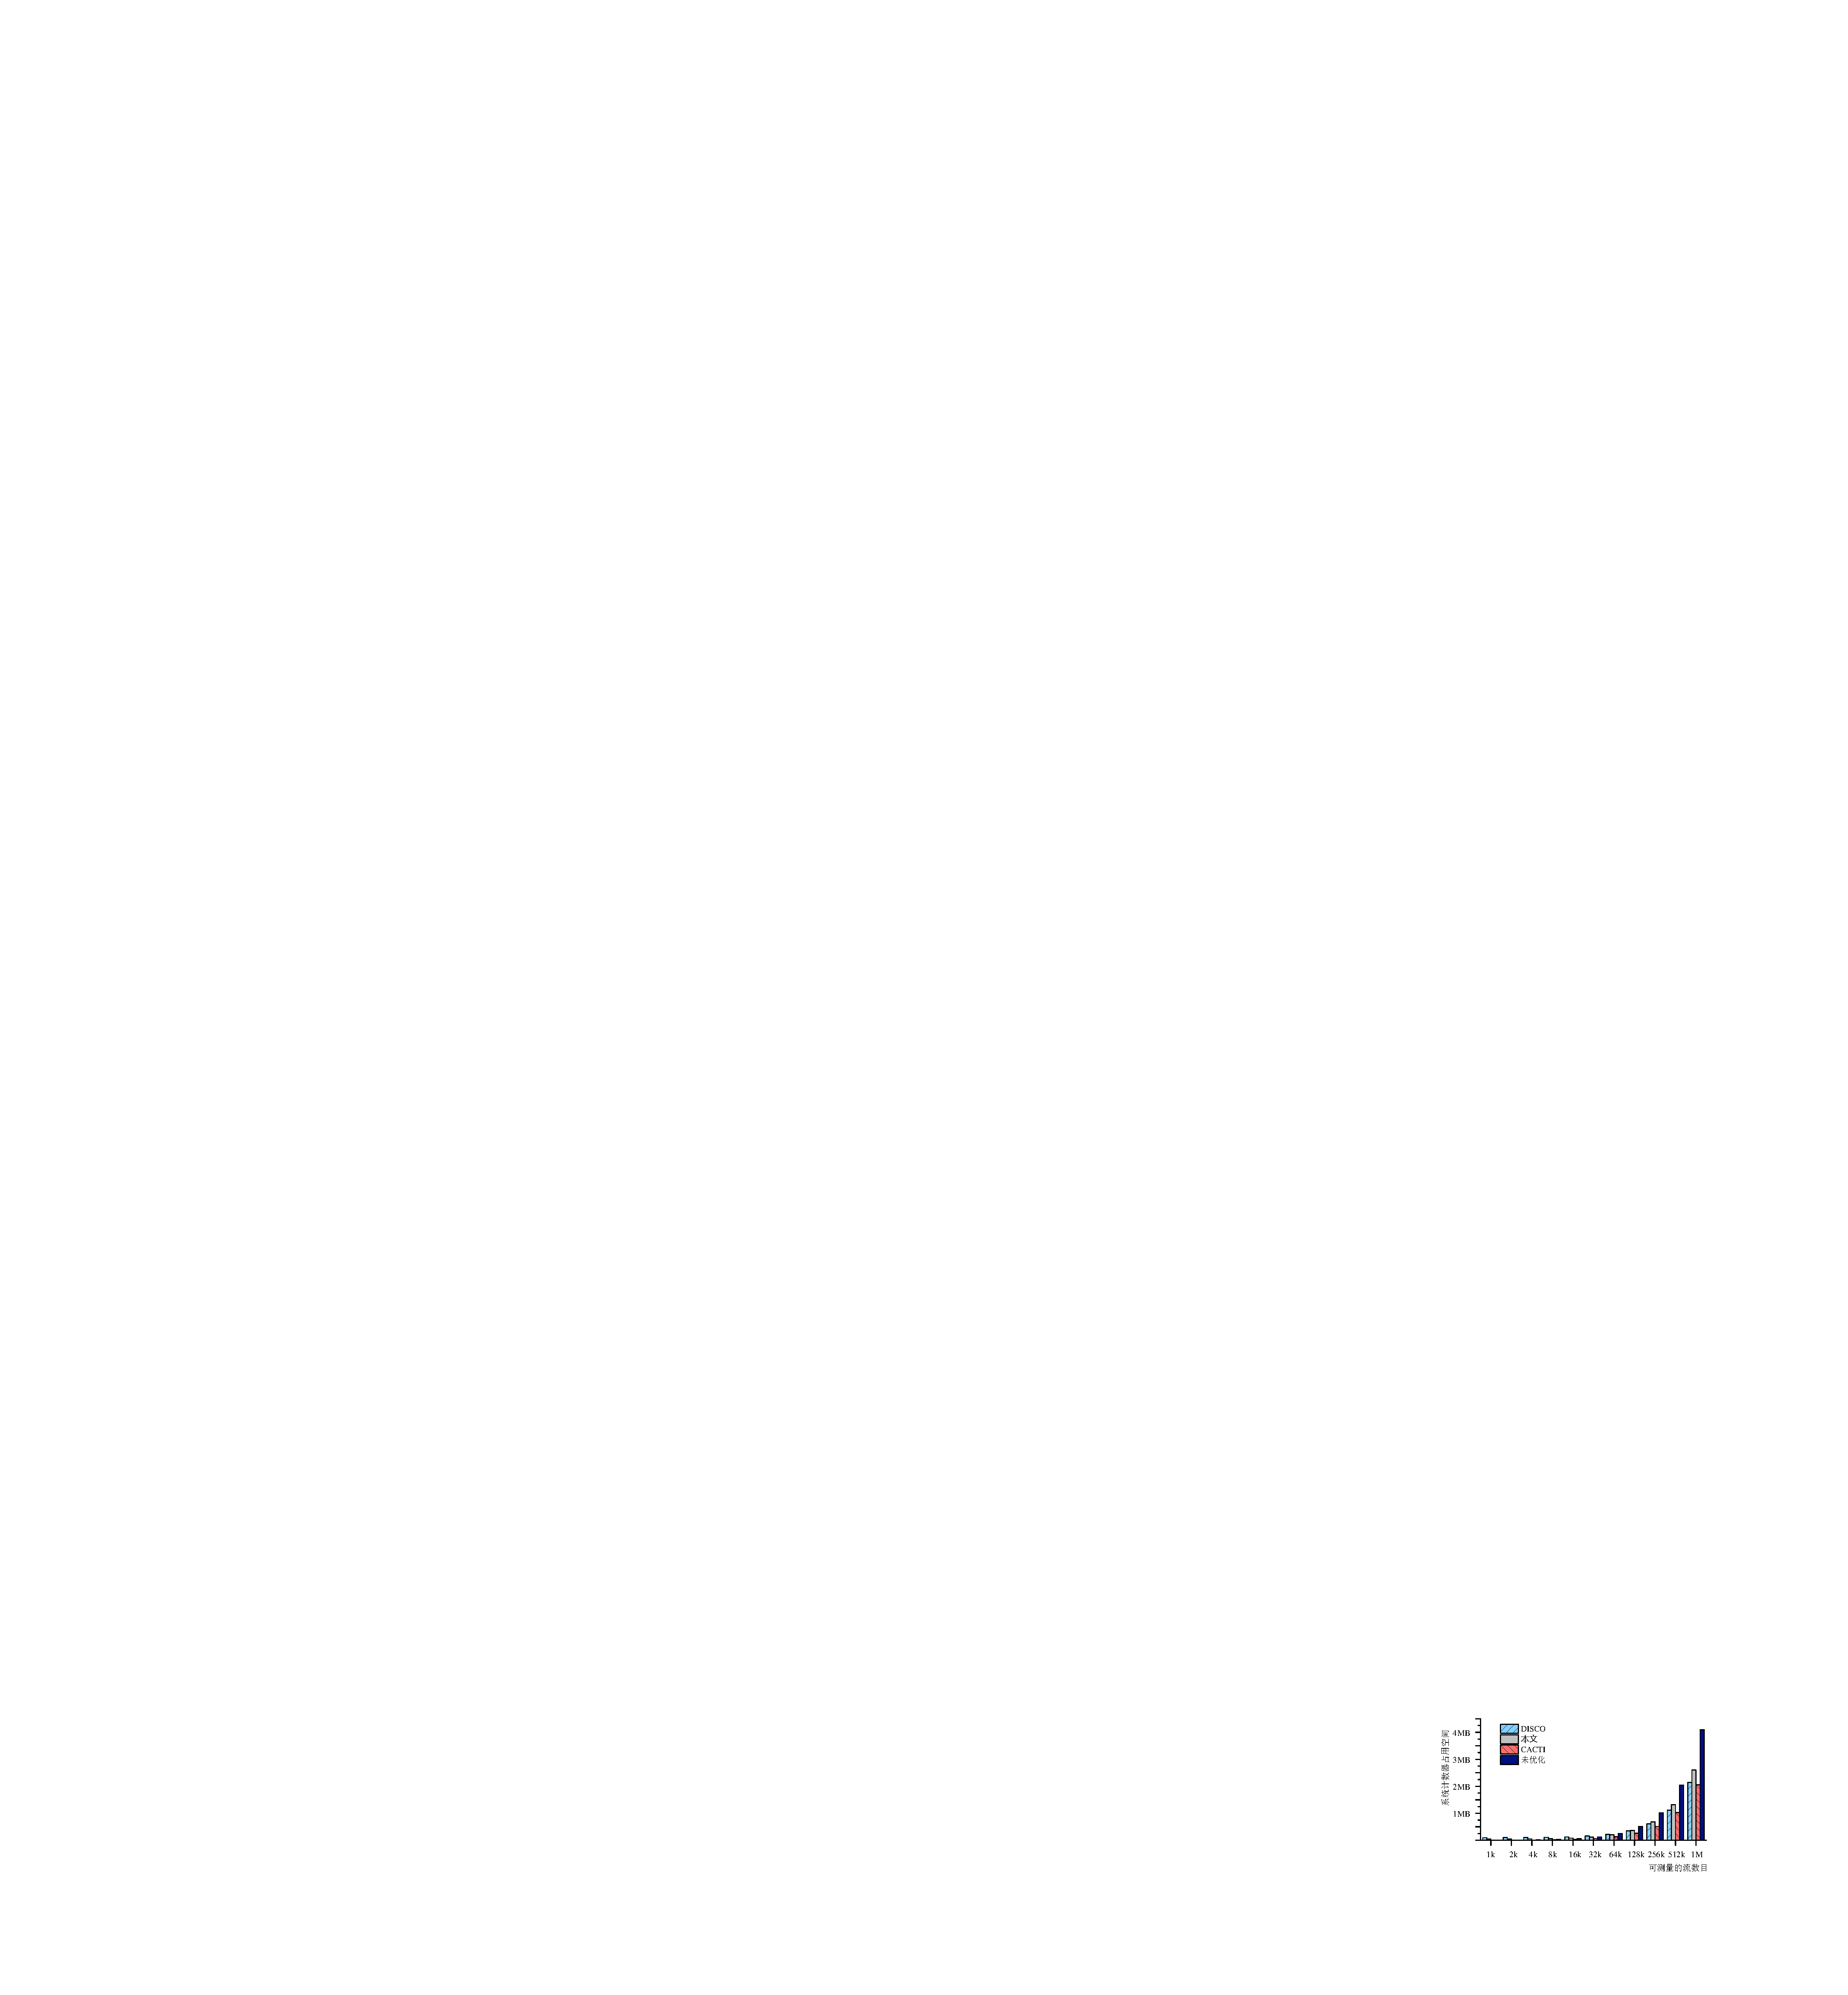
\includegraphics[scale=1]{discomem.pdf}
	\caption{在不同流个数下的压缩计数存储空间占用} \label{fig:discomem}
\end{figure}



4)测量误差。

本文证明基于FPGA的硬件压缩是无偏估计,在统计学中,每一次估计都有估计偏差,本文利用前文\citeup{hu2013discount}提出的估计公式来表示估计偏差,且已经证明变异系数有如下关系:

\begin{equation} \label{mydiscofl}
COV(T(S))=\sqrt{\dfrac{Var[T(S)]}{E^2[T(S)]}}=\sqrt{\dfrac{1-1/n}{2}\times (b-1)}
\end{equation}

其中$ S $为随机变量,代表压缩后的统计值。$ T(S) $为由随机变量$ S $估计的真实统计值。则变异系数即为标准差与平均值之比,变异系数常用于随机过程统计量偏差与误差分析。本文证明压缩估计方法为无偏估计,因而对于同一组序列的估计平均值为常数。则变异系数值越小说明估计值的误差错误比例越低。

\begin{figure}[!ht]
	\centering 
	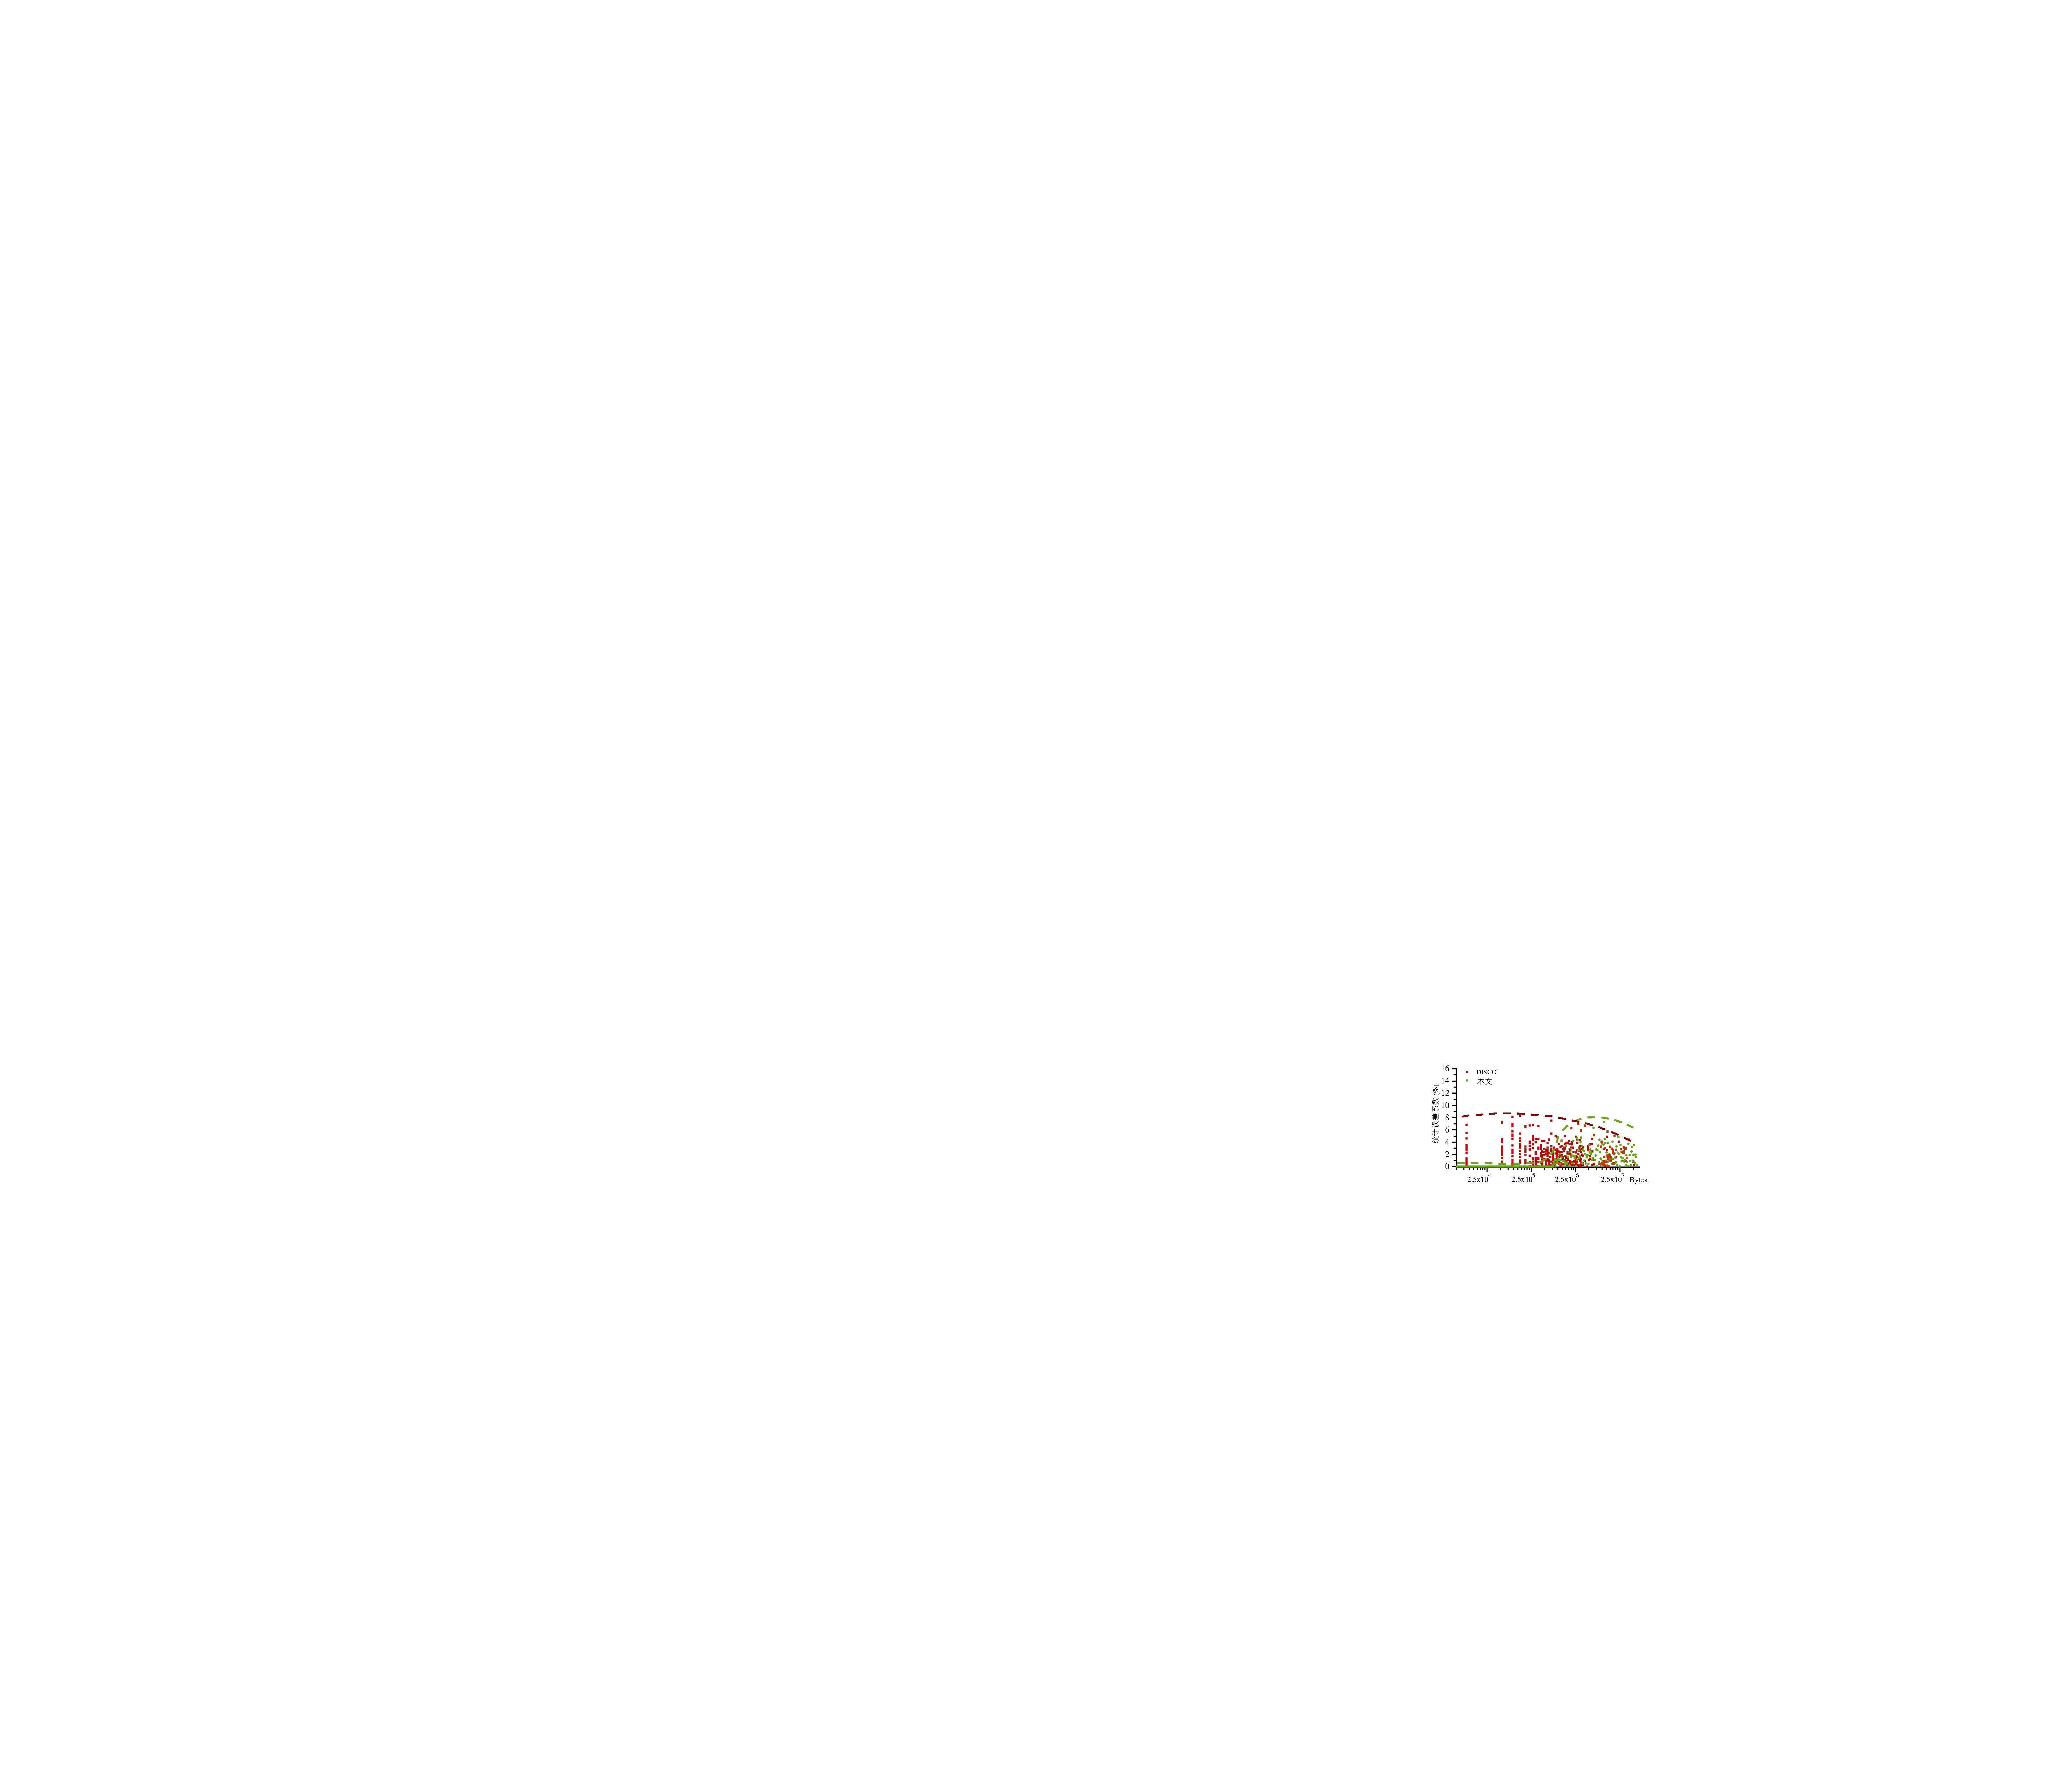
\includegraphics[scale=1]{discoerr.pdf}
	\caption{对不同大小流量估计时的变异系数分布} \label{fig:discoerr}
\end{figure}

%添加误差率的解释,加图,性能加图,解释,然后存储资源图,解释,差不多了。
因为小流的抽样频率低,所以抽样统计在处理小流量时的误差会相对较大。本文在数据流量较小阶段采用线性统计,误差率为零,极大地修复了基于抽象压缩算法的准确性。


\BiSection{本章小结}{aa}

在本章中论文提出了一种基于可编程硬件的智能网卡系统。系统将主机端CPU高耗费的网络应用卸载到可编程智能网卡内,大大缓解了传统网络系统性能低,精度低等问题。为进一步扩展服务器网络性能提供了一种思路和范例。

本文以高时间精度,高计算密集度的网络应用为例,设计了一套高性能的流量捕获,统计,回放系统。在网络安全,流量监测领域可提供性能支持。本文将网络协议栈时间控制精度由目前的几微秒提高到20纳秒。另外本文提出一种基于硬件的带有压缩存储空间容量的流量统计工具,根据本文提出的硬件加速设计DC抽象方法,本文将目前基于软件的25Gbps性能提升到133Gbps吞吐;同时可压缩相应的高性能存储空间40\%的占用量,并显著改善了统计精度。根据本文提出的系列算法,将测量系统的灵活性、资源消耗率与高性能合理折中。由于功能卸载后效率更高,本文所耗费的CPU资源几乎比之前工作下降了100\%。















